\chapter{Section 2} \label{section2}
\section{Outline of Implemented Features}
Prior to proceeding with the sketch, it was necessary to define which panels would be utilized in the application. In accordance with the recommendations provided by the professor, the decision was made to create five panels. The following panels were created: Situation Panel, Log Panel, Cameras Panel, Resources Panel and Auxiliary Screens. \par
For each panel, an analysis was conducted to identify the most pertinent characteristics to be considered. In regard to the Situation Panel, it was determined that an essential preliminary step would be the utilization of a map of the district, in conjunction with the delineation of the locations of the fires and their respective conditions. \par
When considering the Log Panel, it was determined in advance that the ability to select, aggregate and filter data, such as contract or expand information, would be beneficial in facilitating the interpretation of the available information. \par
In relation to the Camera Panel, it was established that the panel would contain six cameras, and that it would be advantageous to have the ability to manipulate these, for example, by zooming in, panning left and right, and moving up and down. Furthermore, it was hypothesised that it would be advantageous to have the option of capturing an image of the visualisation currently being displayed by the camera. \par
When considering the Resources Panel, it is evident that the aspect of localization is of significant importance, as is the communication between the civil protection operator and the fire-fighting resources that would be in operation, including air, ground and human resources. These resources may include fire crews, tankers, reconnaissance vehicles, heavy or light bomber helicopters and seaplanes, among other. \par
It is also essential that the Auxiliary Screens are capable of adapting to the specific functionalities required by each of the preceding panels. To illustrate, the ability to select, enlarge a camera or map, handle the panels or display pertinent information in greater detail would be beneficial. \par
In consideration of the preceding factors, the initial sketches were formulated, which are presented below in a systematic arrangement by panels. %\par
\begin{itemize}
    \item \textbf{Situation Panel}: 
        \begin{itemize}
            \item Single:
            \begin{figure}[H]
                \centerline{%
                \subfloat[Sketch 1]{
                    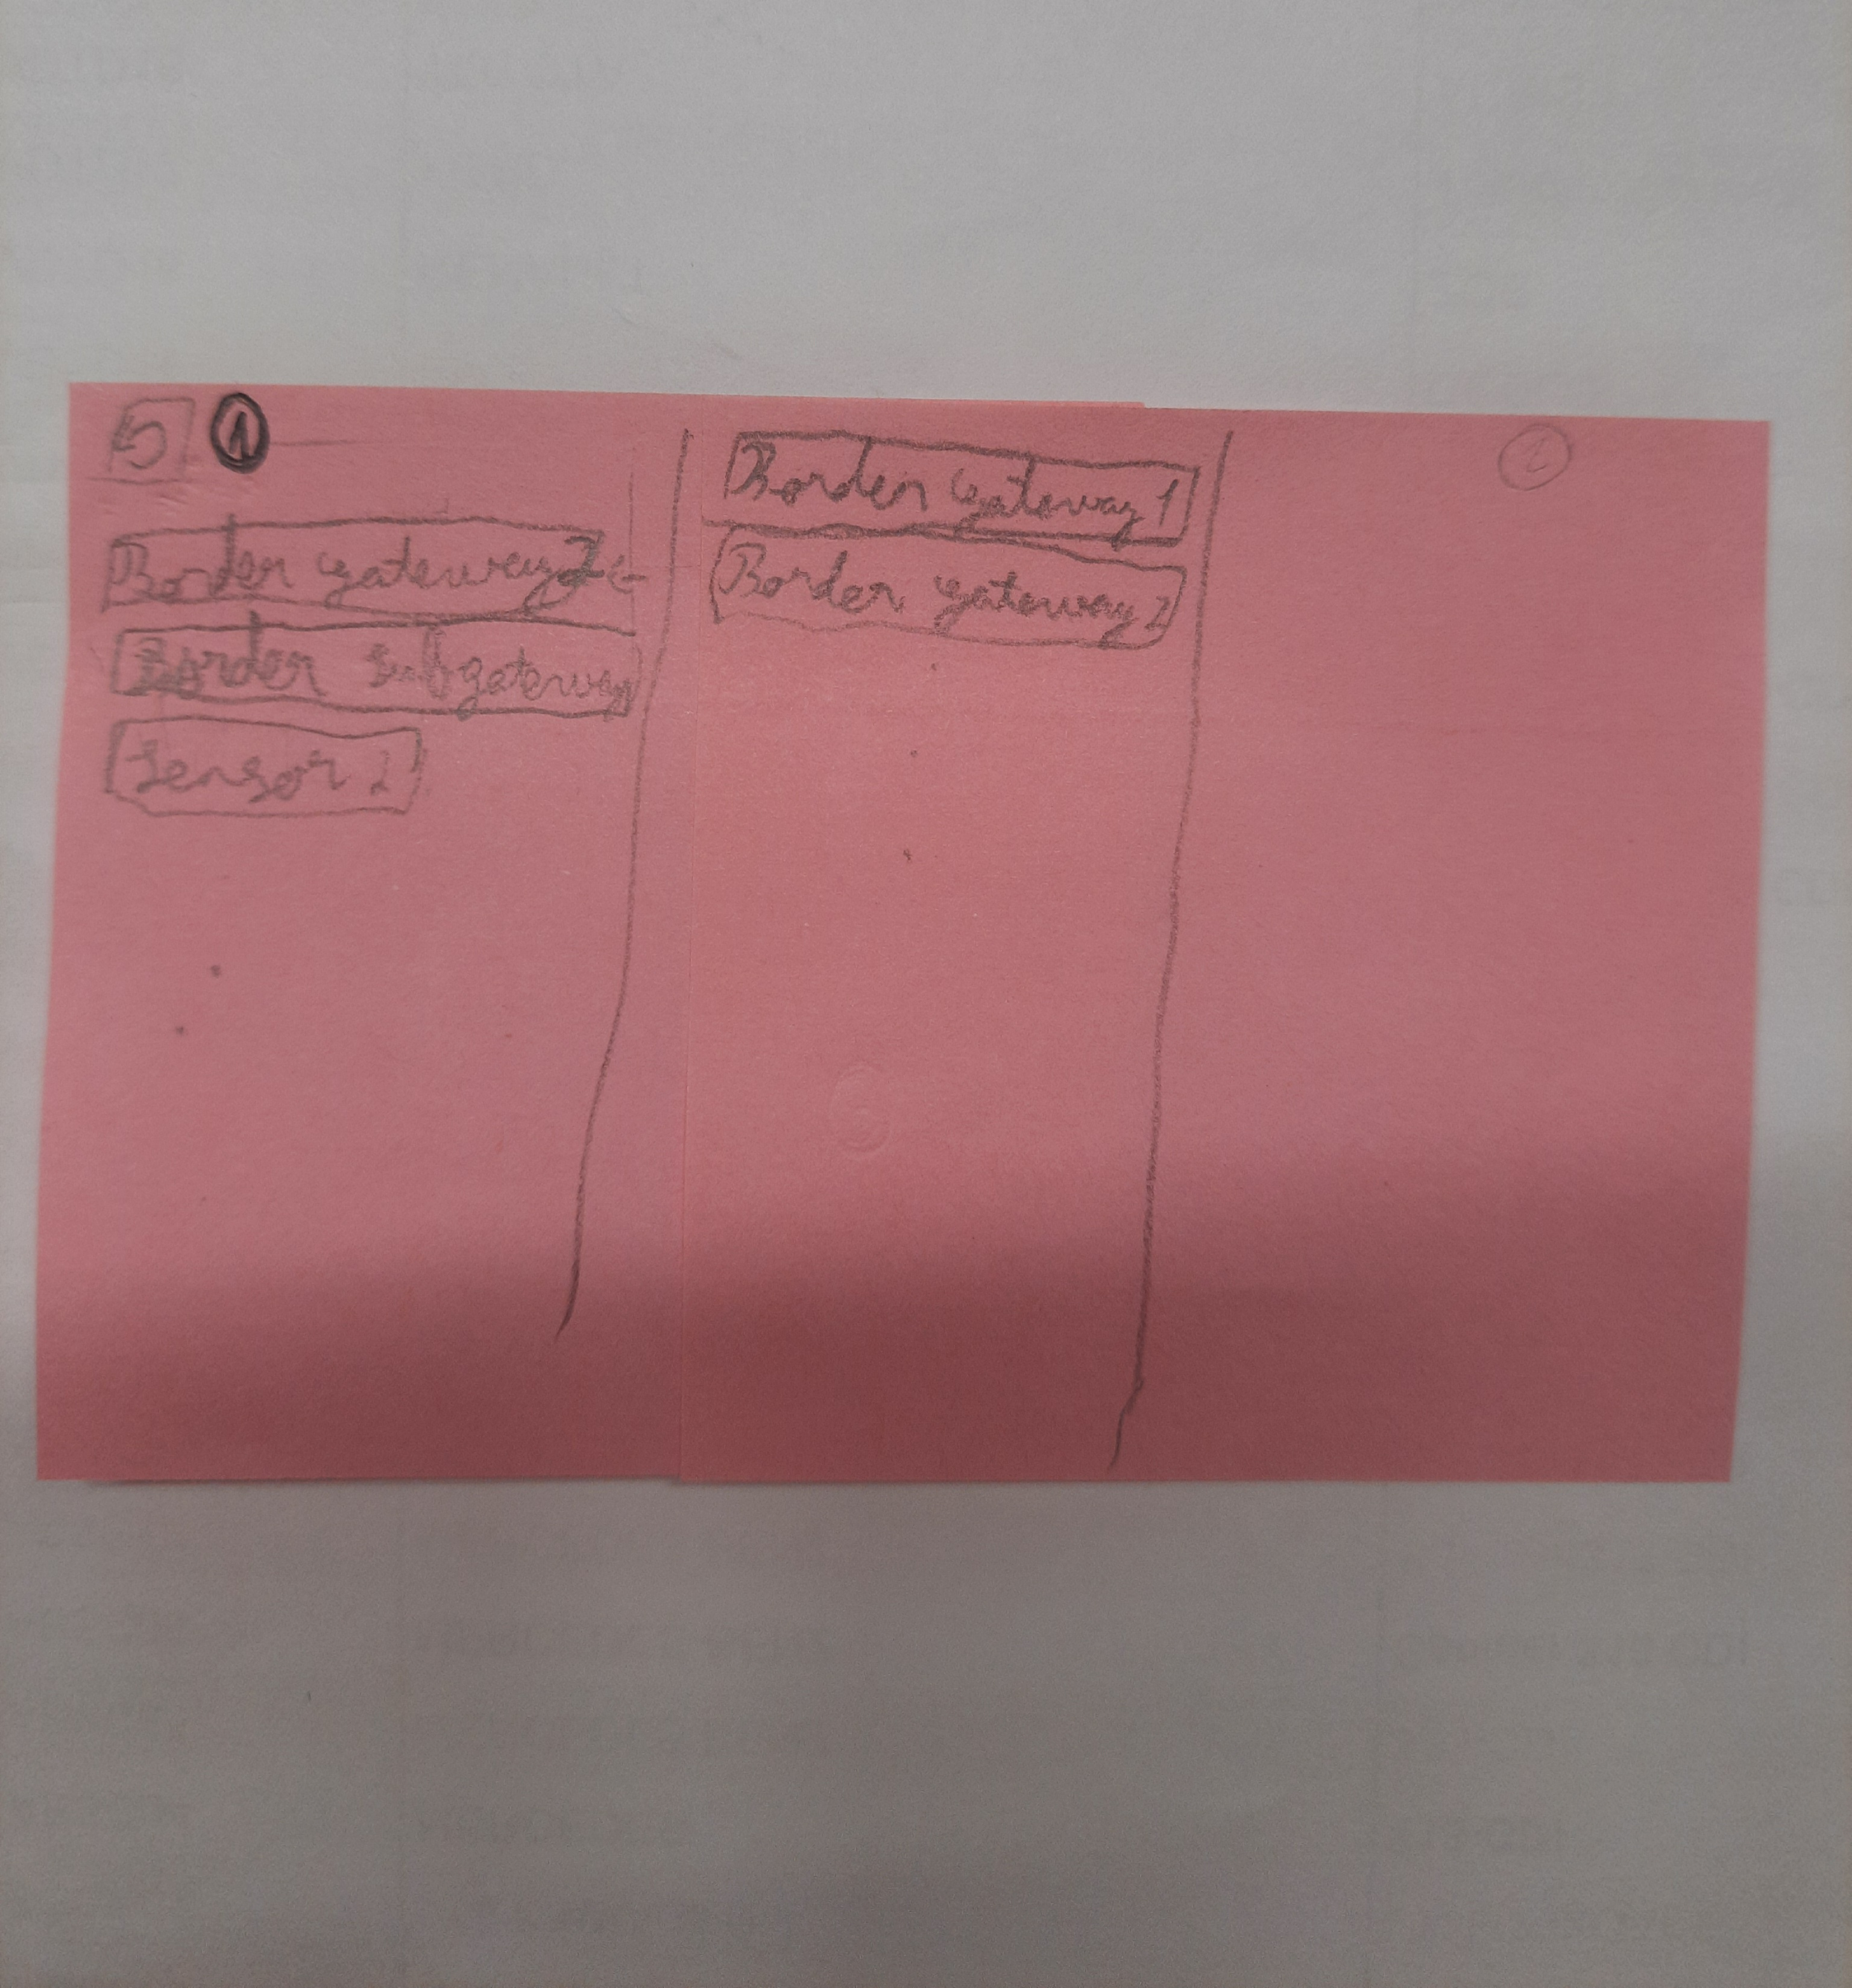
\includegraphics[width=.5\textwidth]{sketches/Situation_1.jpg}
                }\hfill 
                \subfloat[Sketch 2]{
                    \begin{turn}{270}
                    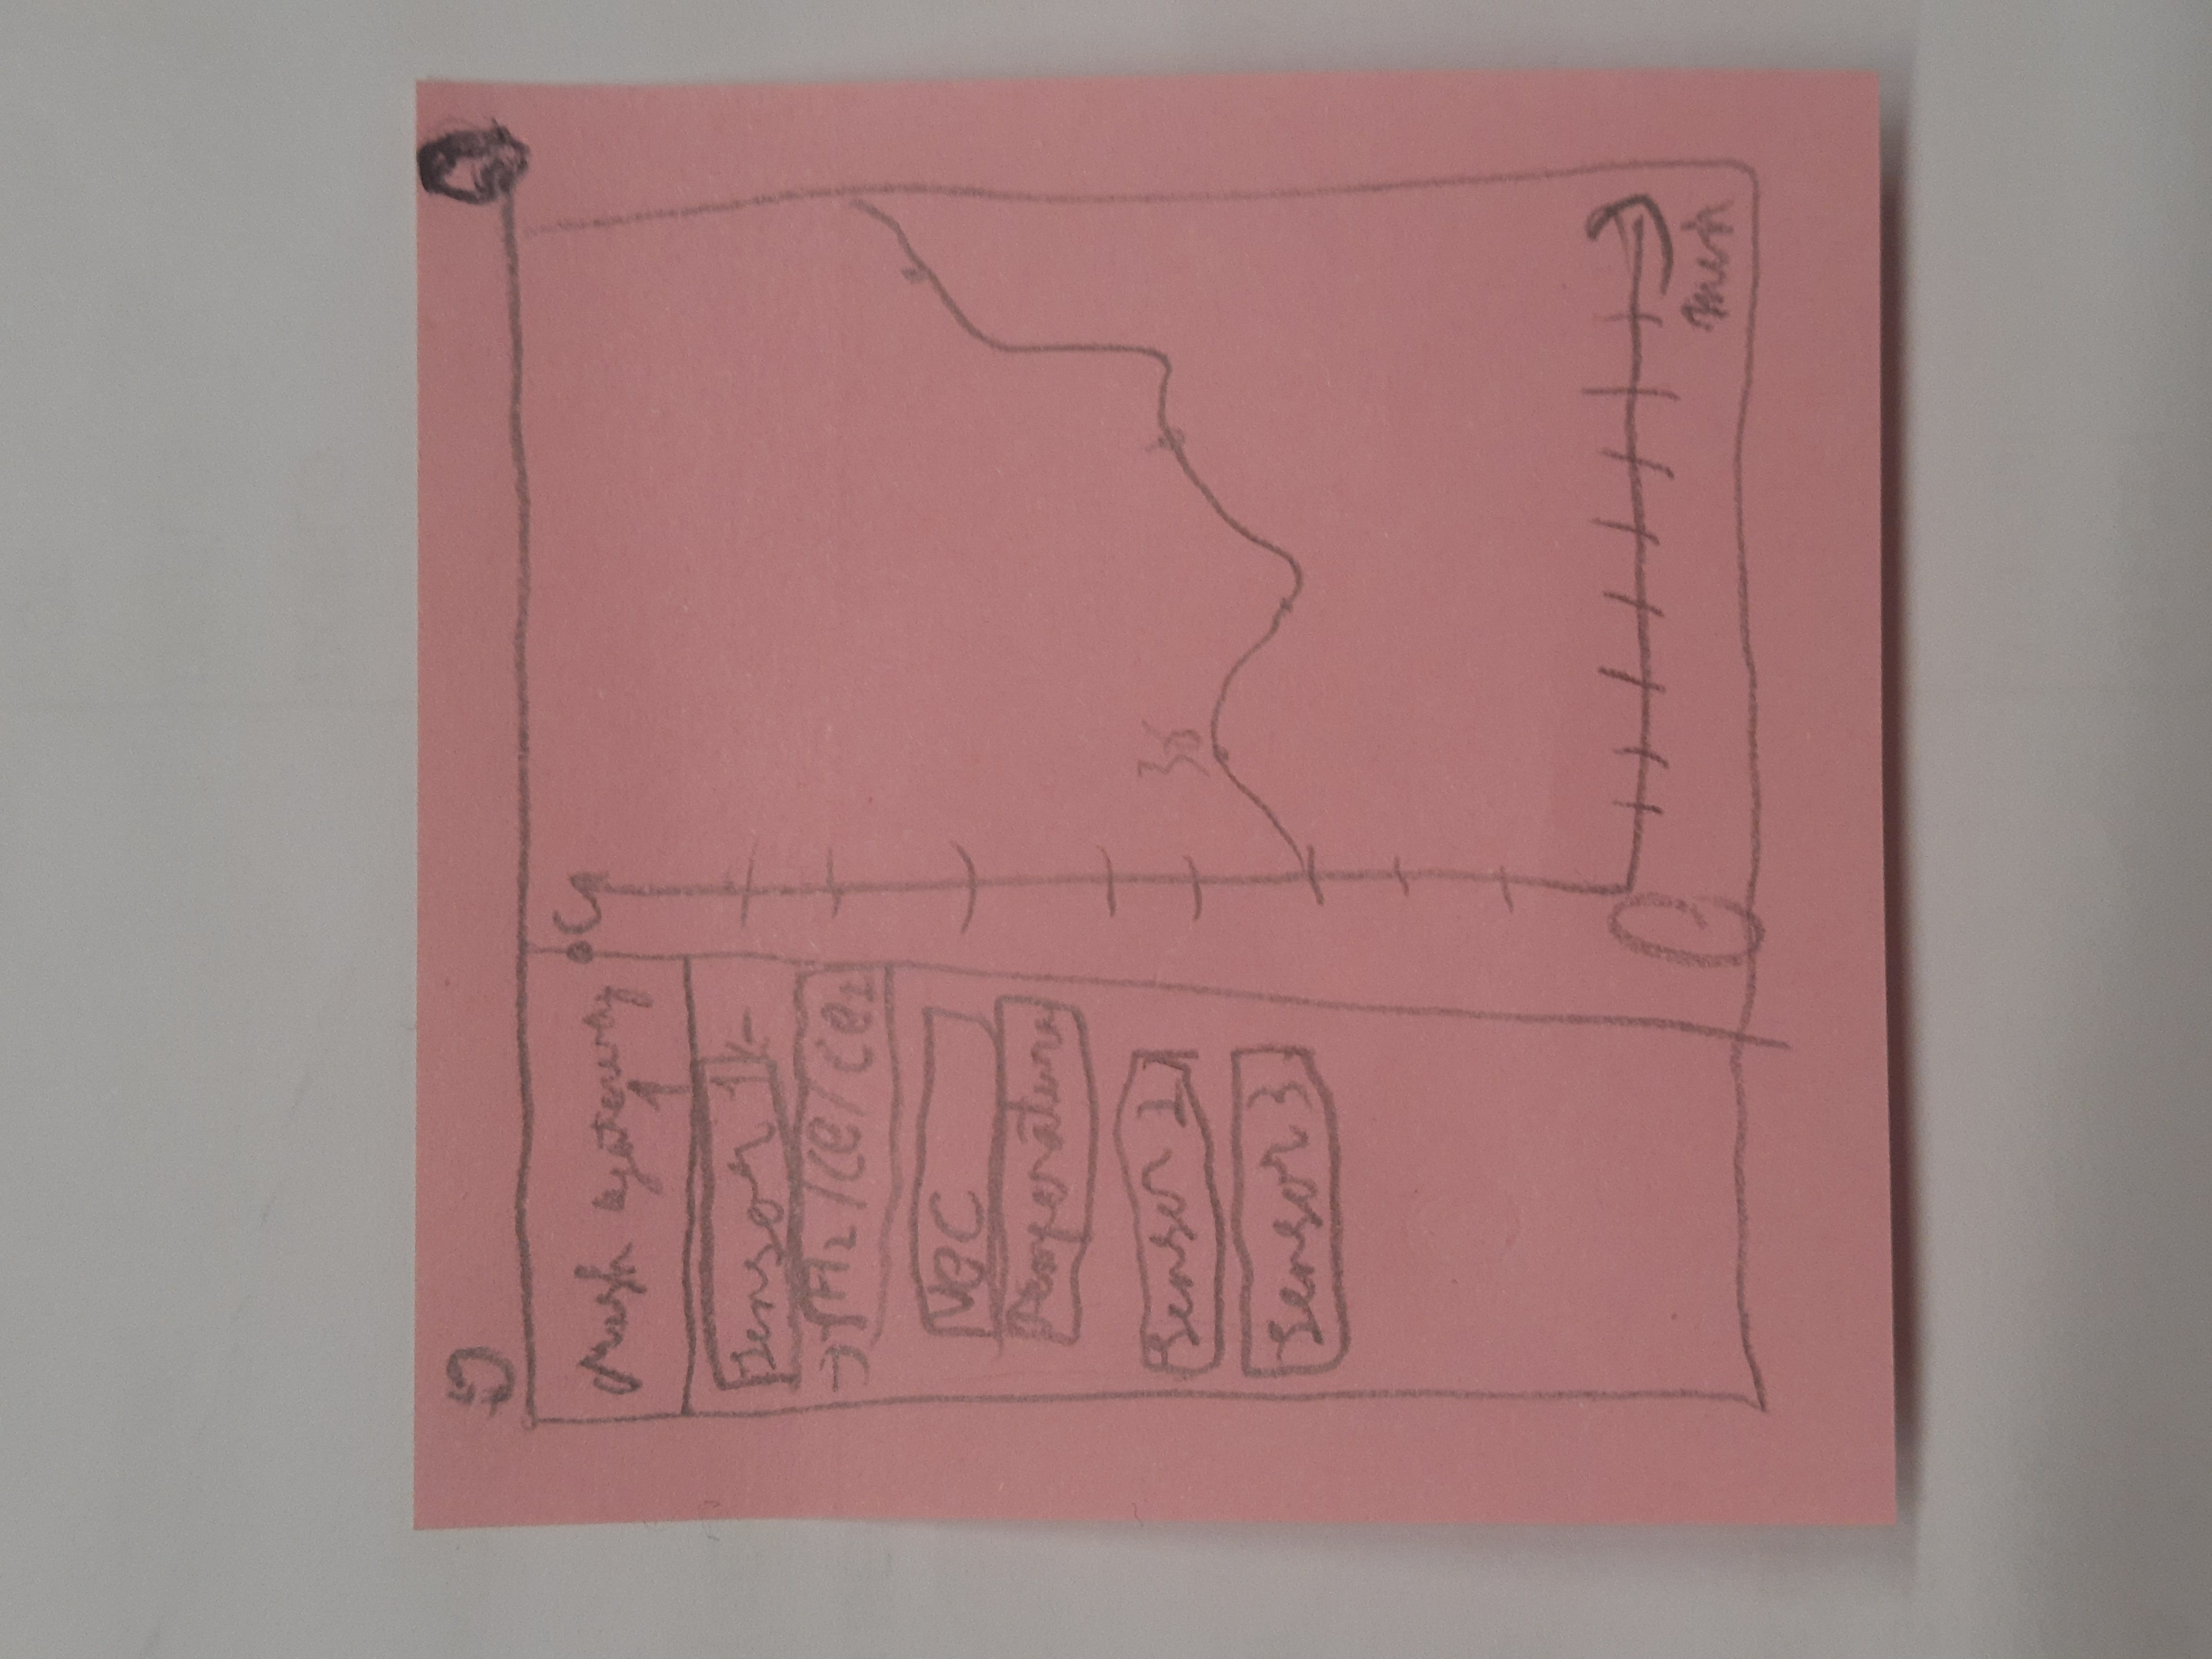
\includegraphics[width=.5\textwidth]{sketches/Situation_2.jpg}
                    \end{turn}
                }\hfill 
                \subfloat[Sketch 3]{
                    \begin{turn}{270}
                    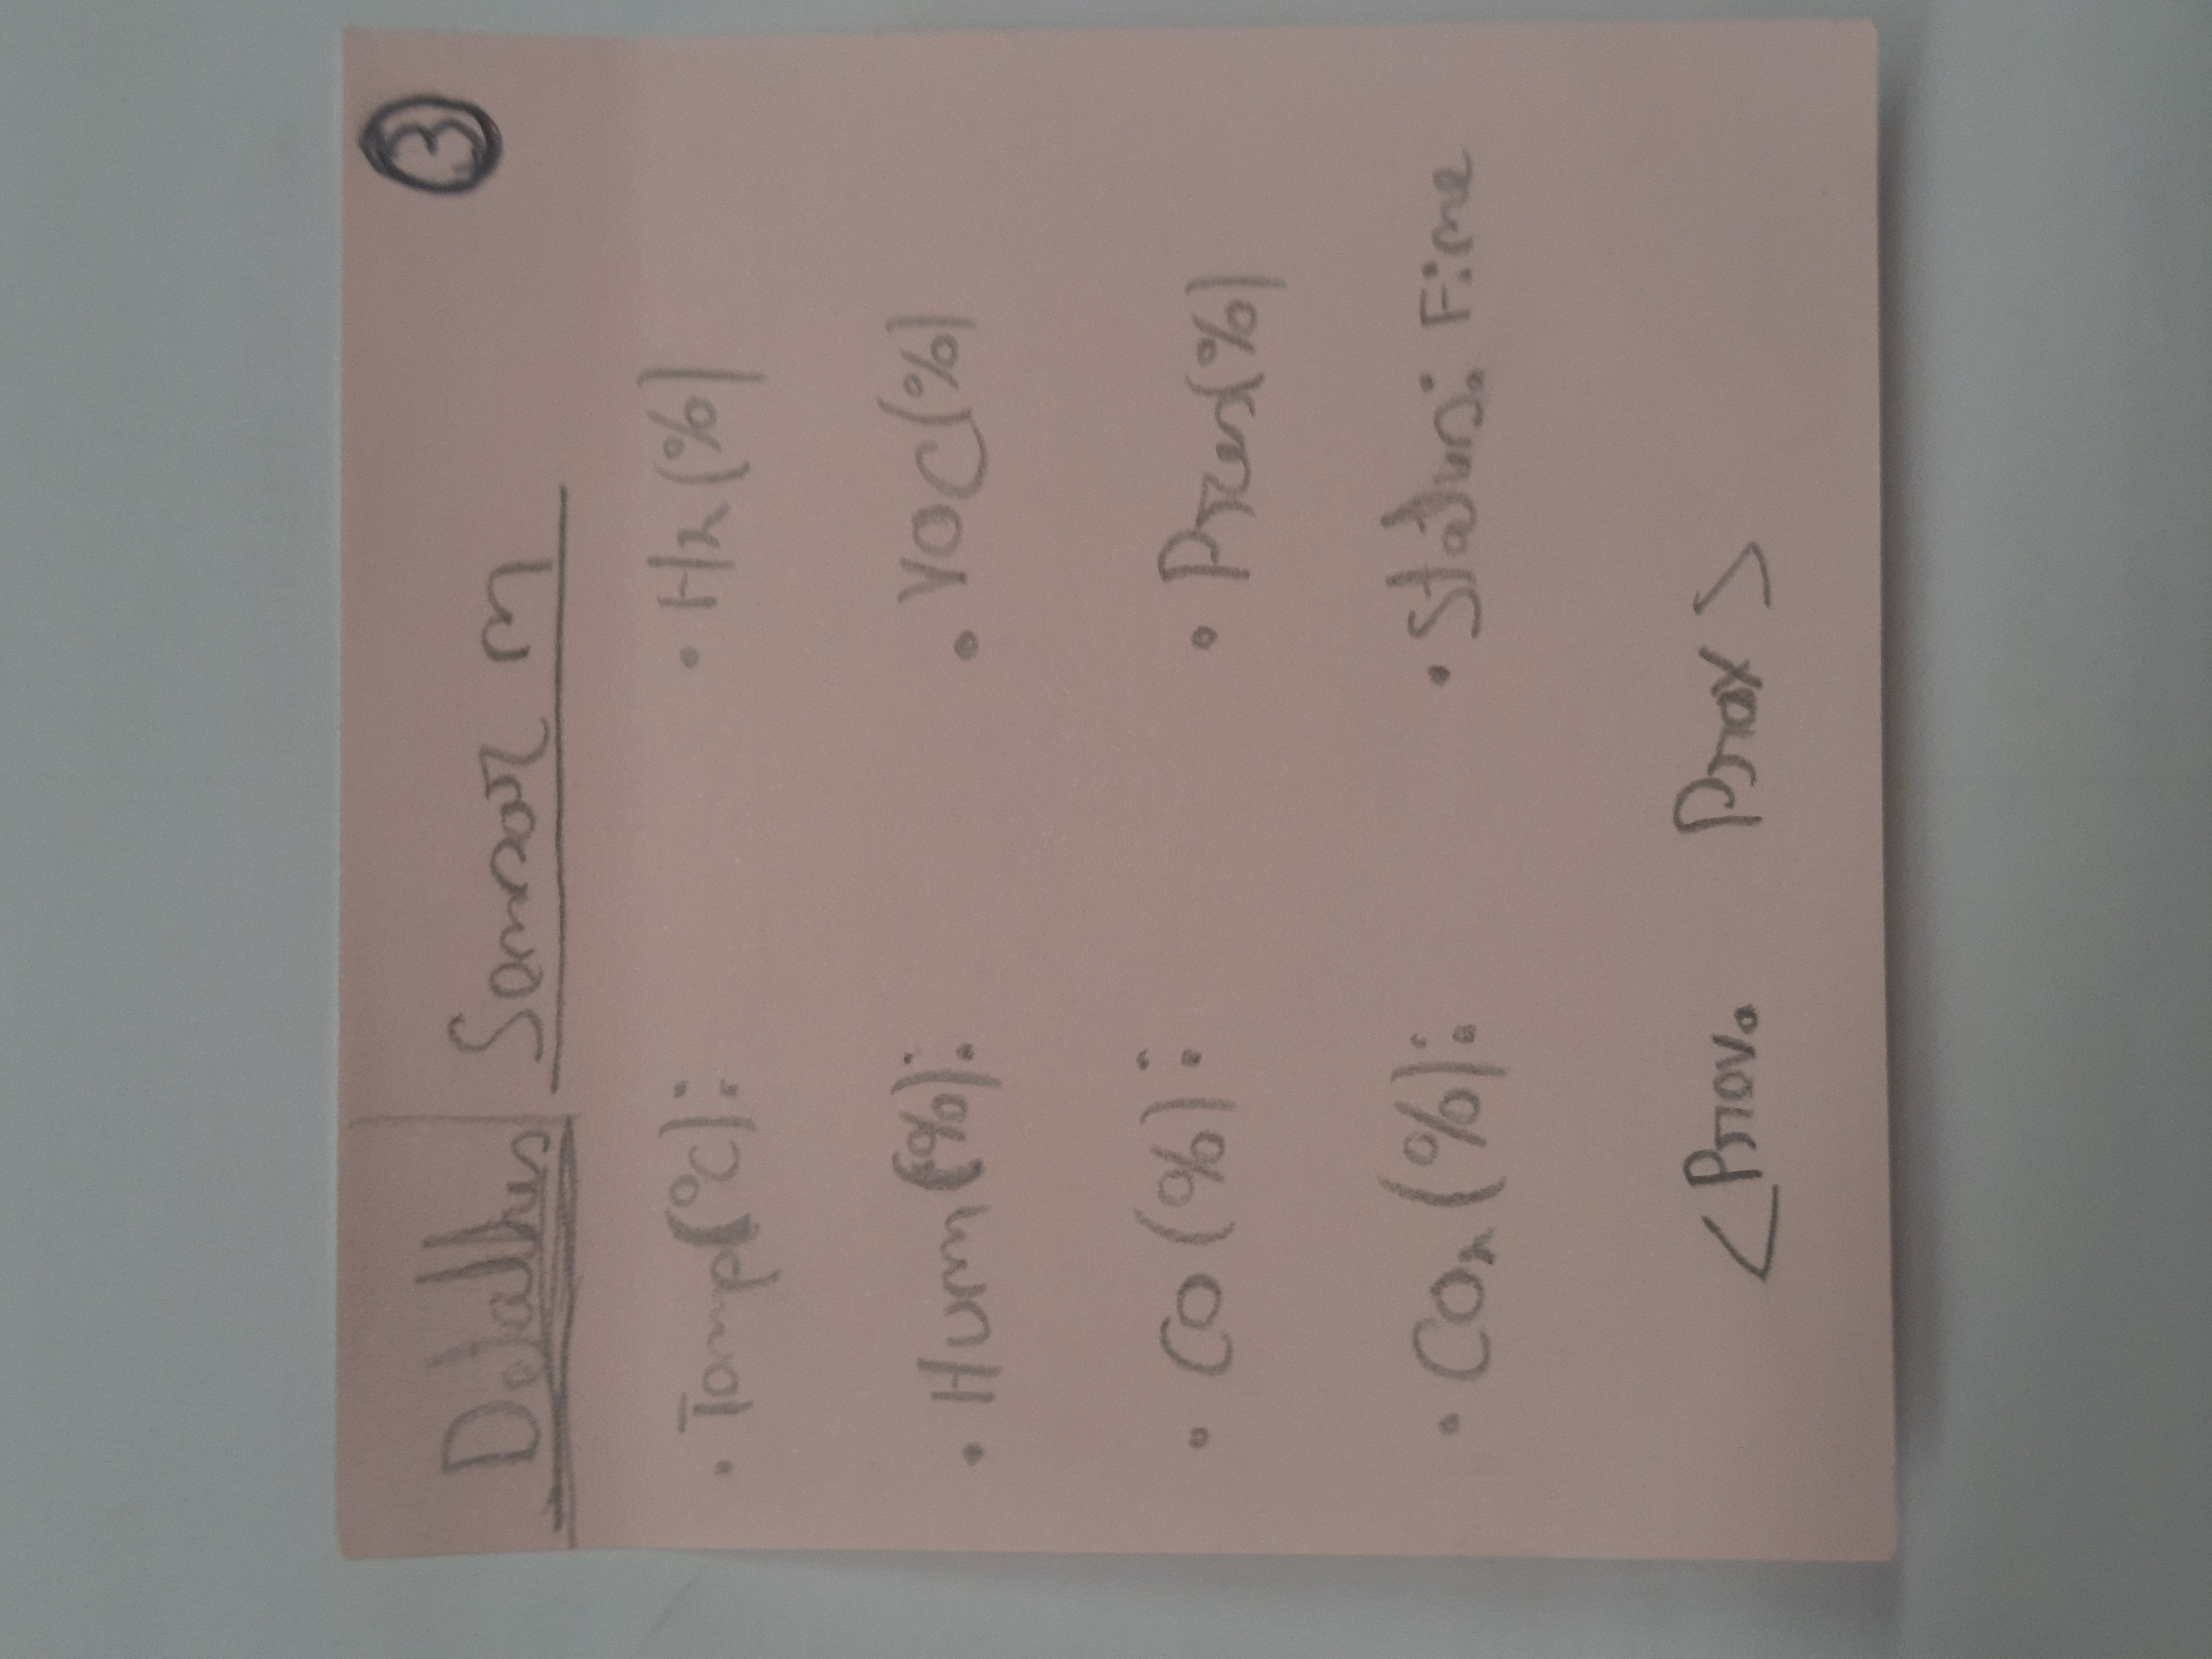
\includegraphics[width=.5\textwidth]{sketches/Situation_3.jpg}
                    \end{turn}
                }%
                }
                \centerline{%
                \subfloat[Sketch 4]{
                    \begin{turn}{270}
                    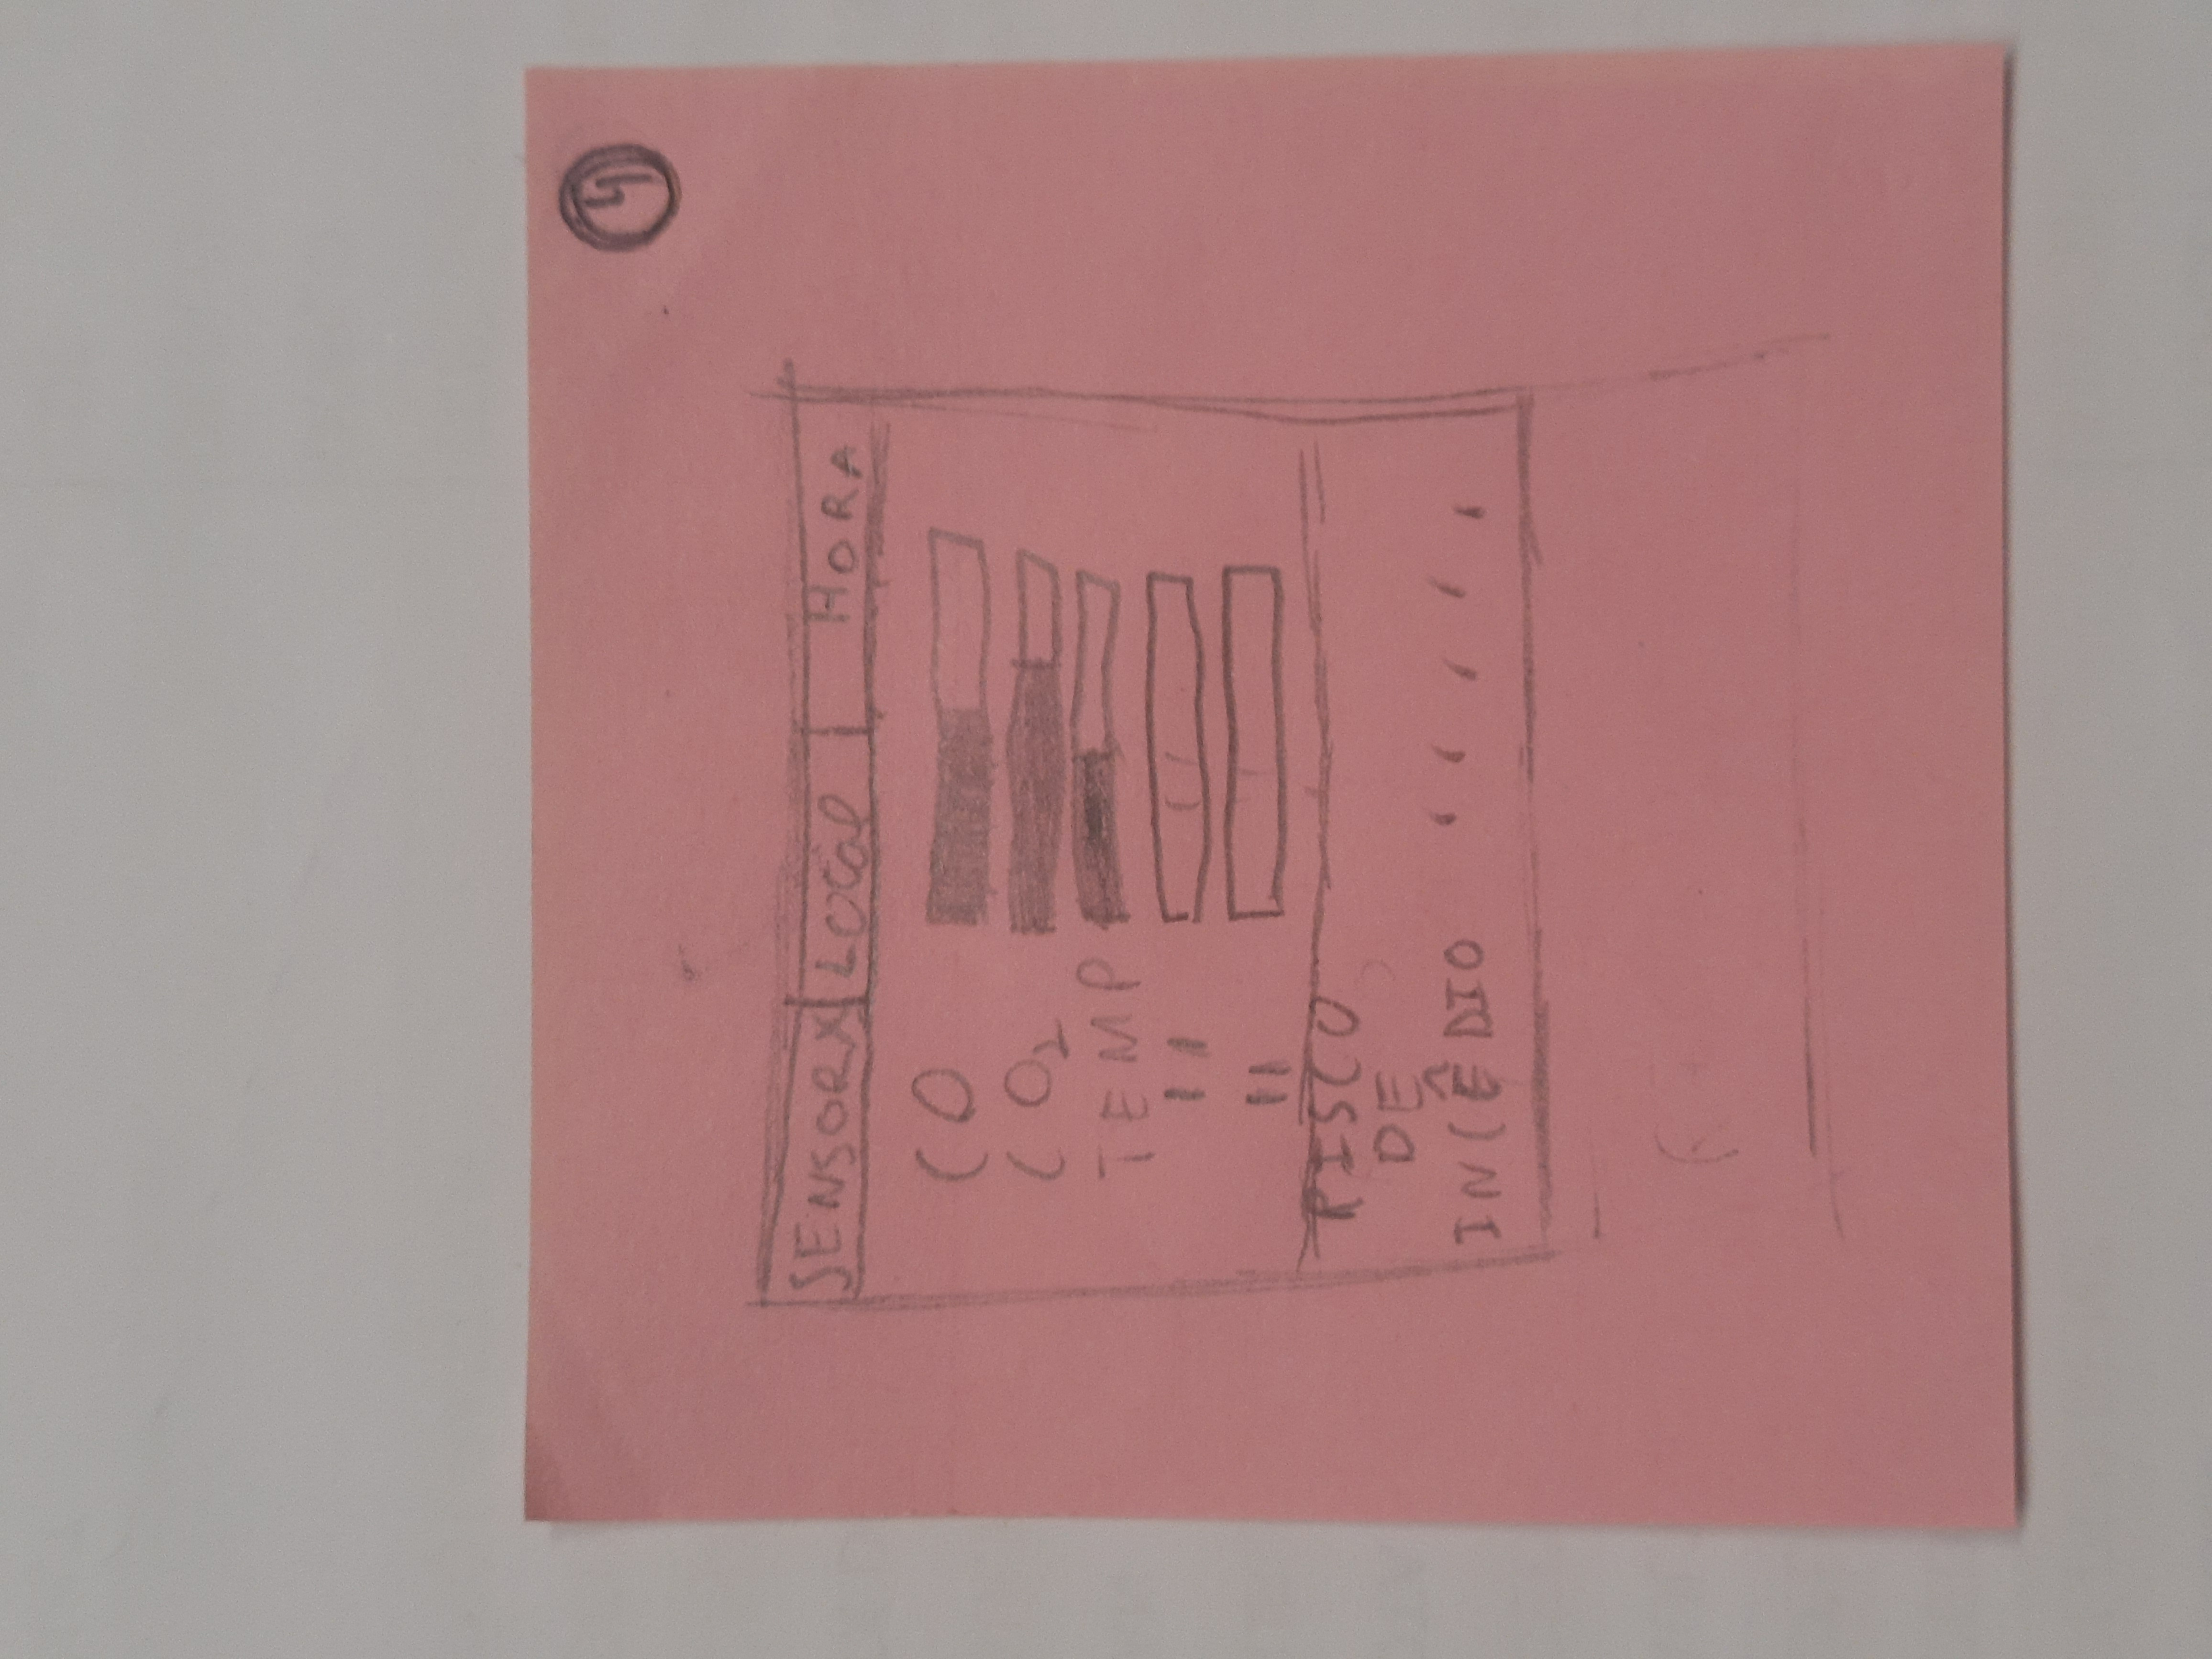
\includegraphics[width=.5\textwidth]{sketches/Situation_4.jpg}
                    \end{turn}
                }\hfill 
                \subfloat[Sketch 5]{
                    \begin{turn}{270}
                    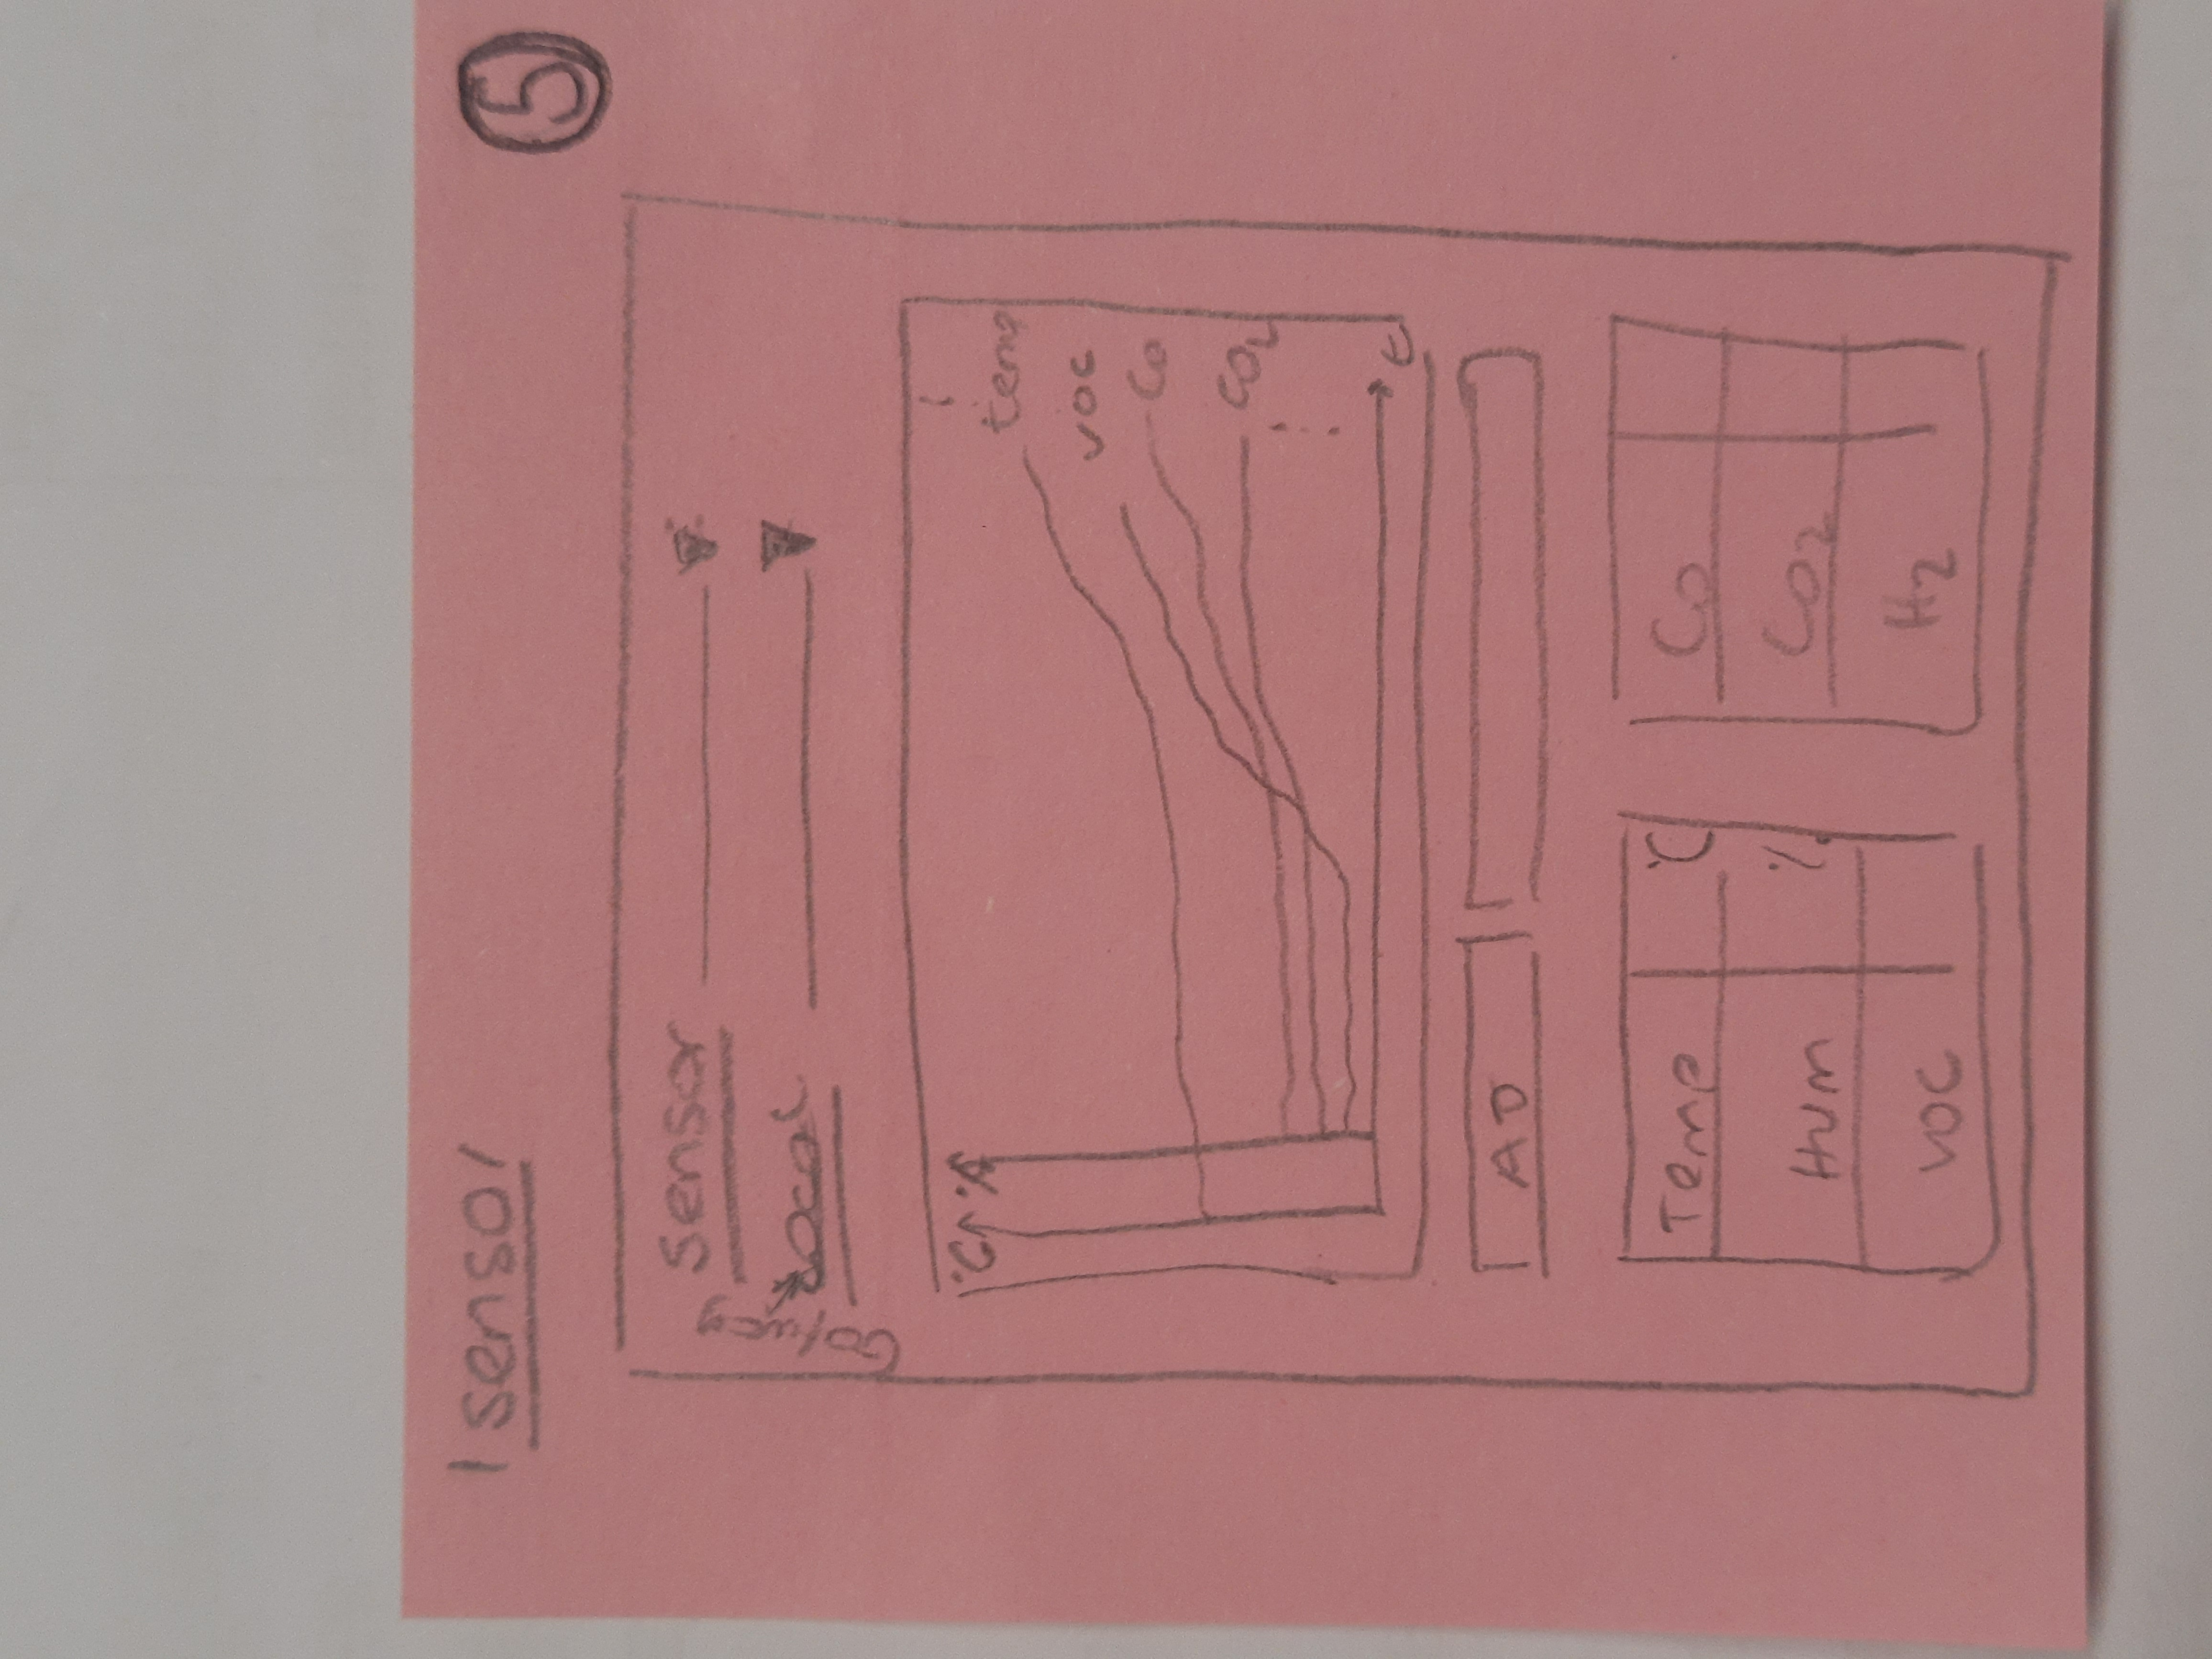
\includegraphics[width=.5\textwidth]{sketches/Situation_5.jpg}
                    \end{turn}
                }\hfill 
                \subfloat[Sketch 6]{
                    \begin{turn}{270}
                    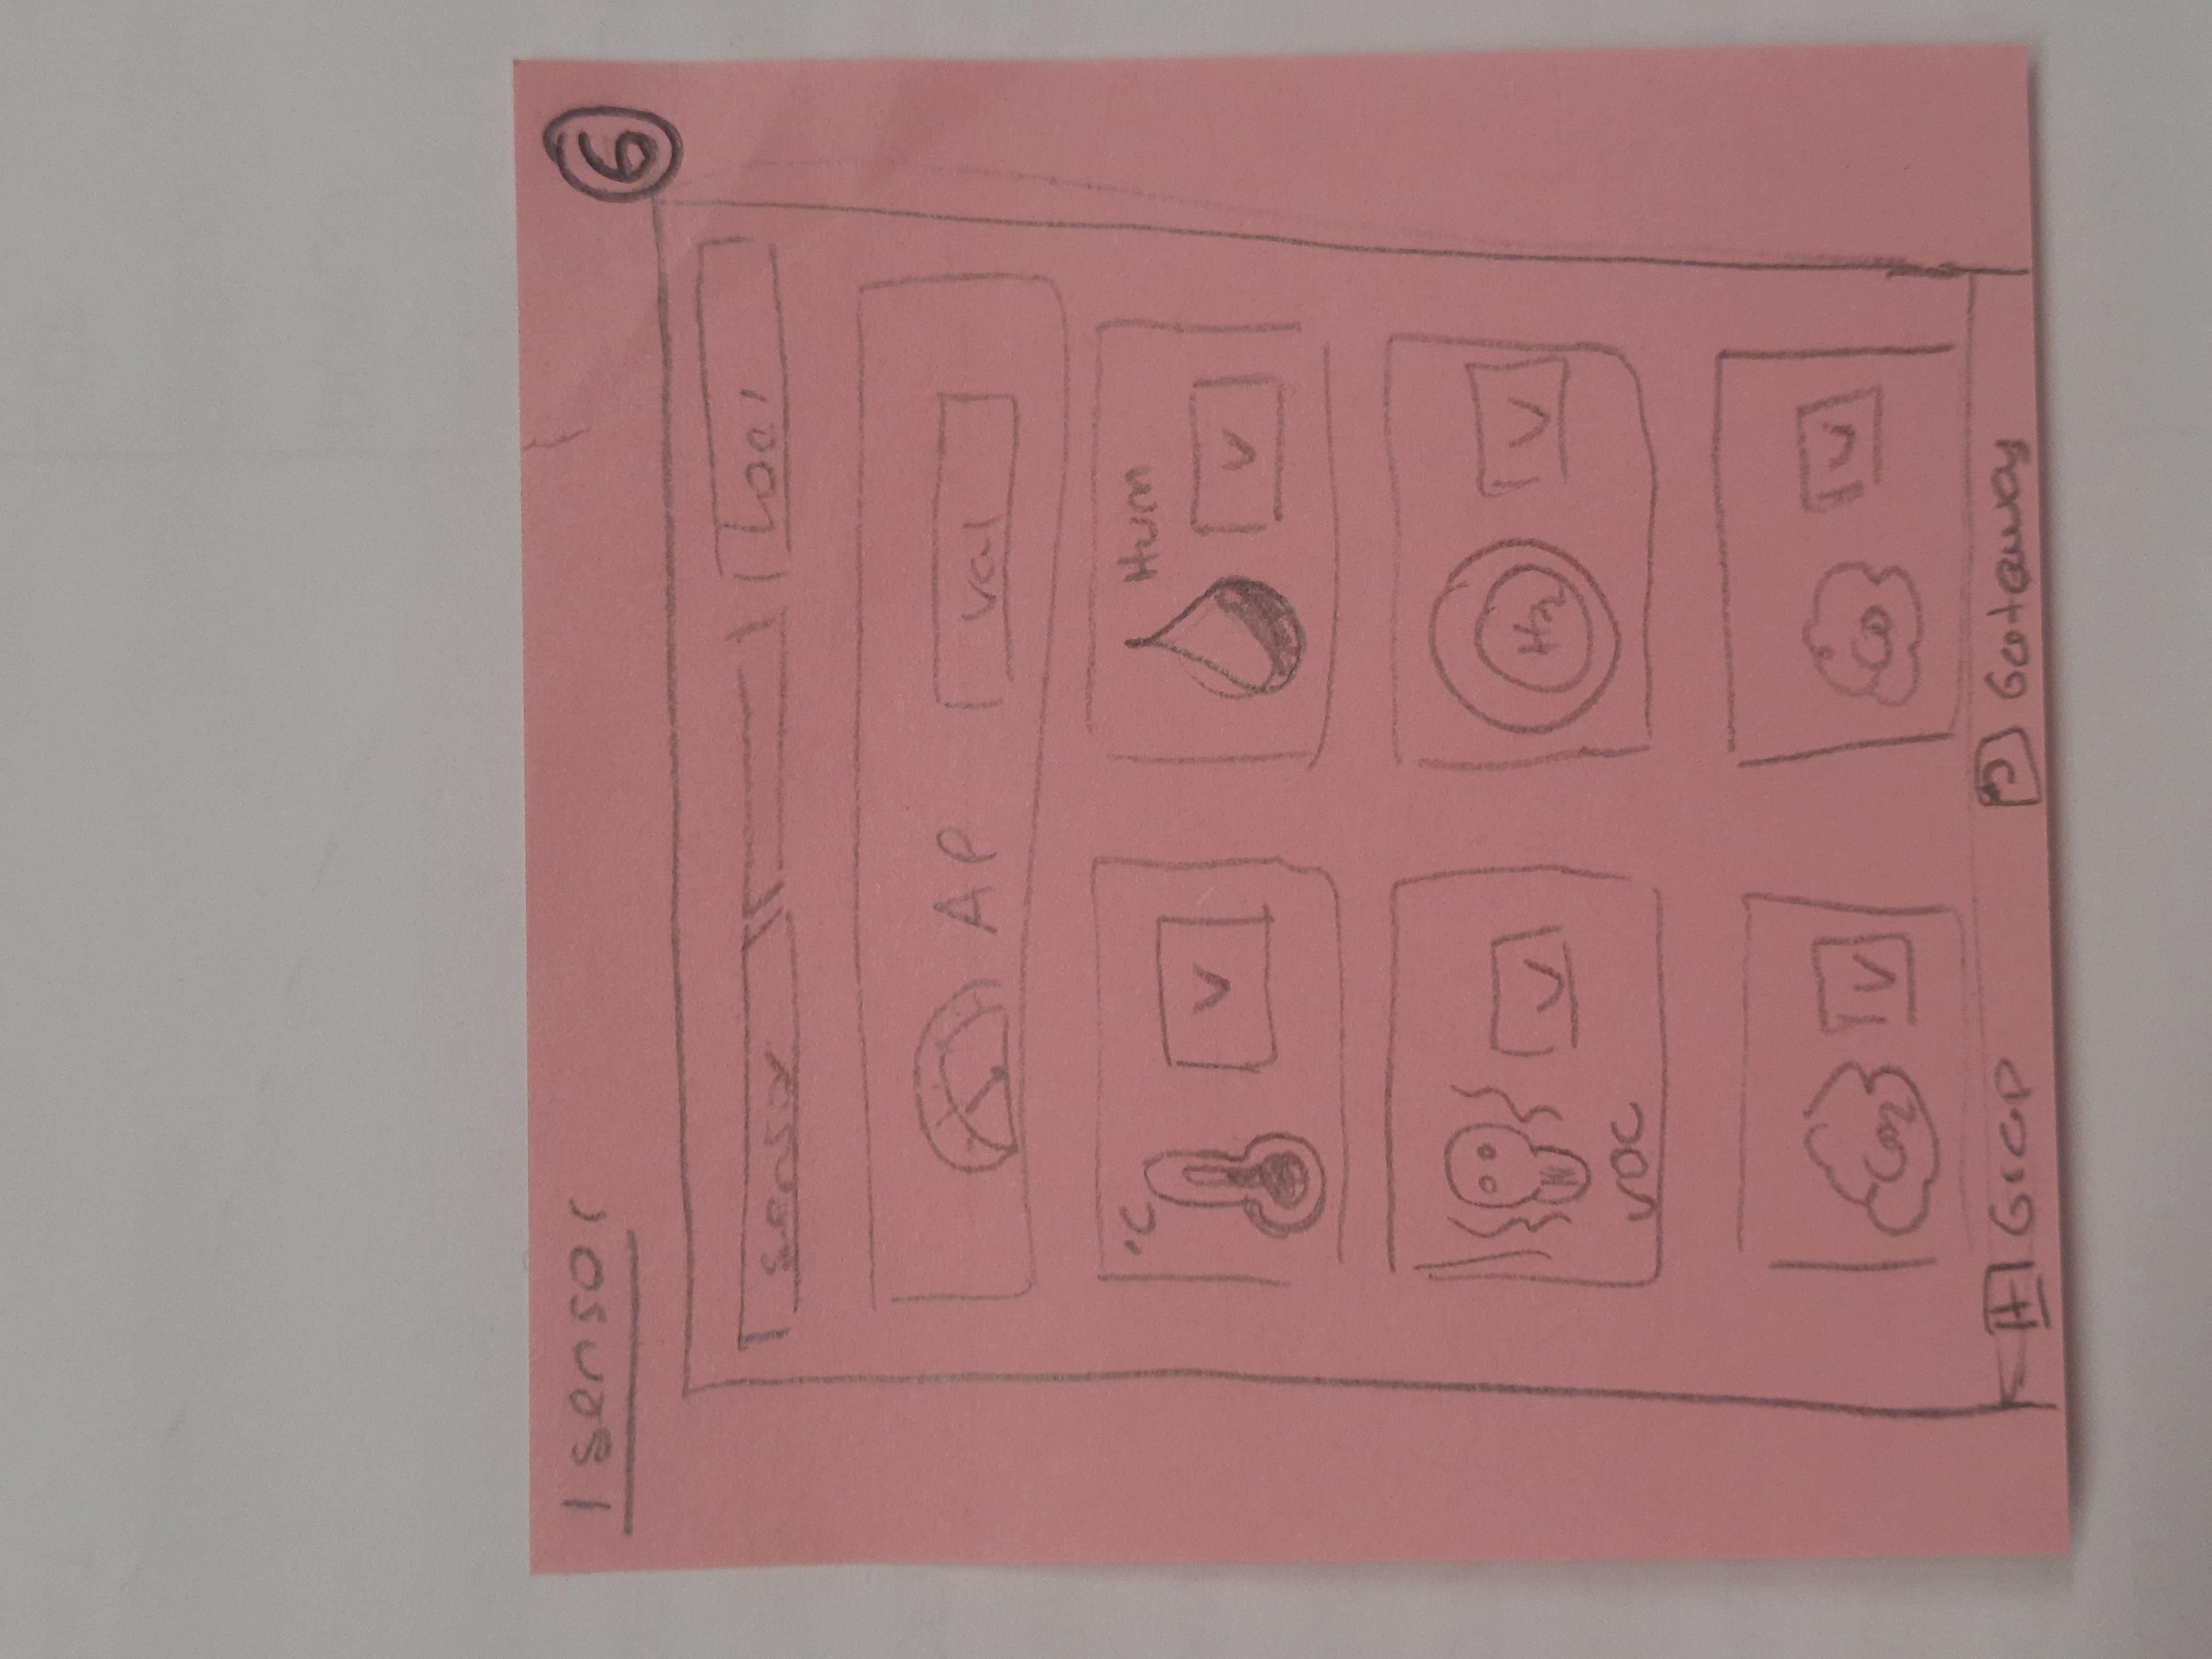
\includegraphics[width=.5\textwidth]{sketches/Situation_6.jpg}
                    \end{turn}%\hfill
                }%
                }
                %\end{figure}
                %\begin{figure}[H]\ContinuedFloat
                    \centerline{%
                \subfloat[Sketch 7]{
                    \begin{turn}{270}
                    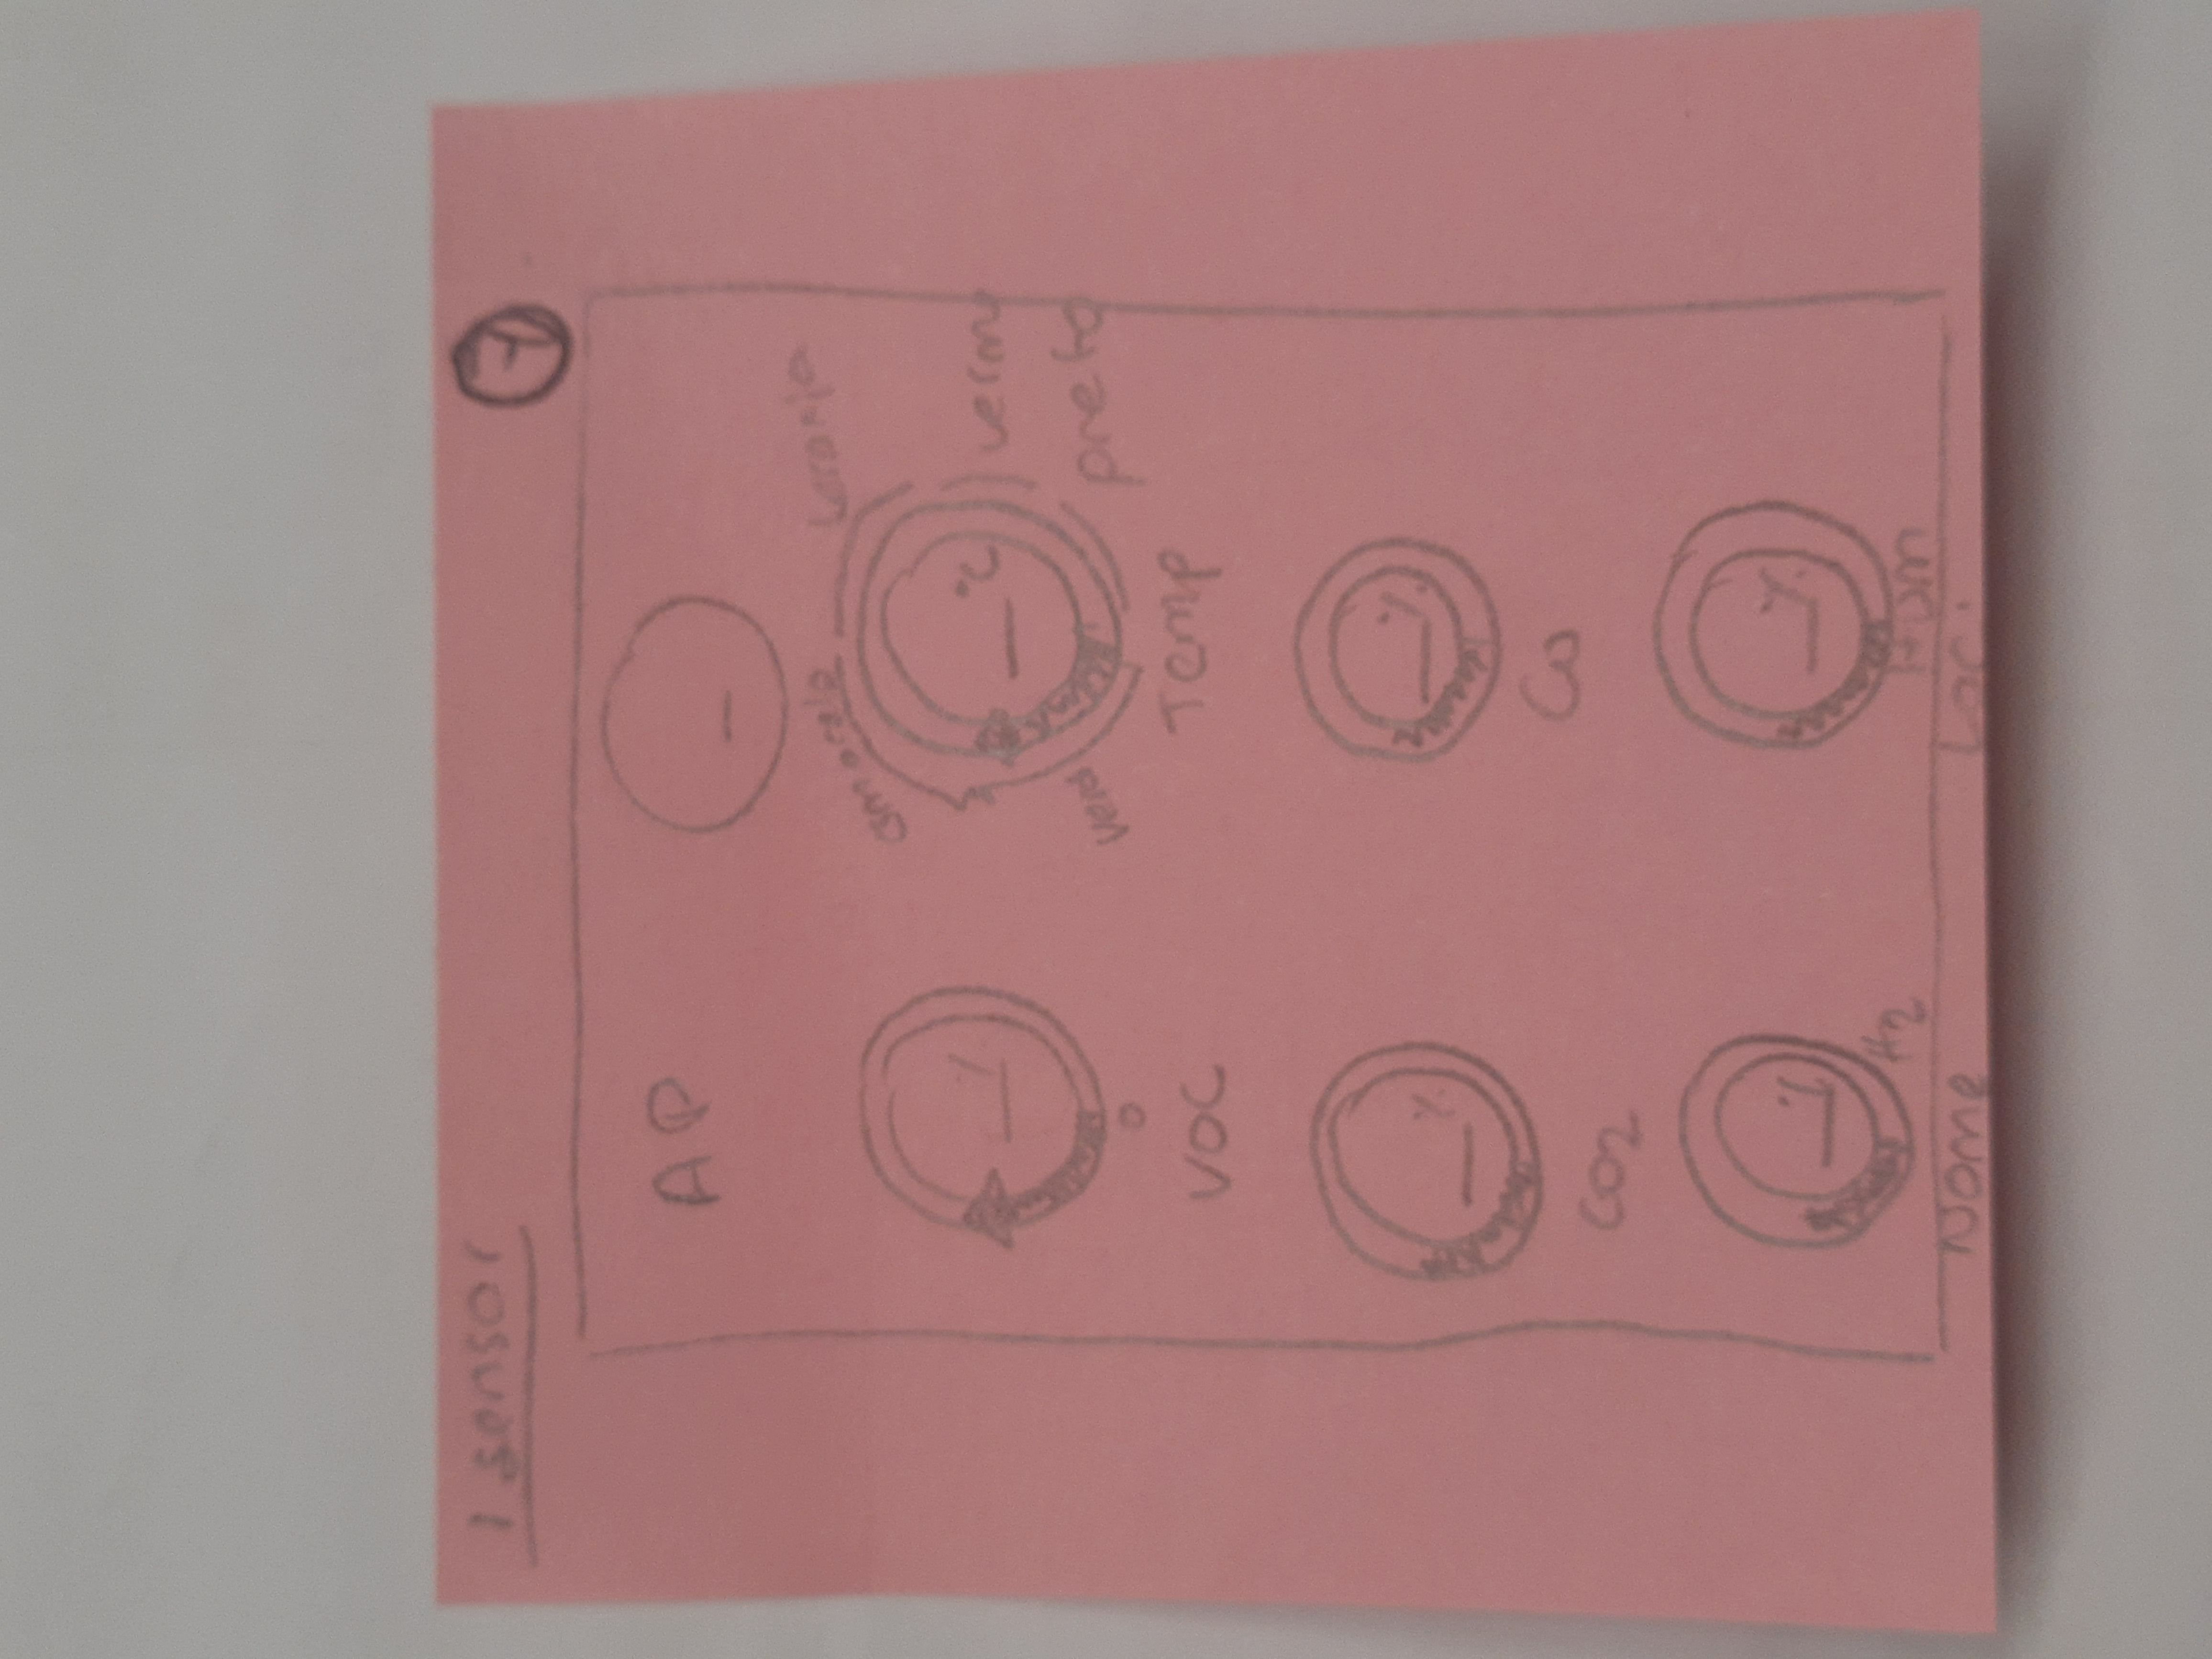
\includegraphics[width=.45\textwidth]{sketches/Situation_7.jpg}
                    \end{turn}\hfill
                }
                \subfloat[Sketch 8]{
                   \begin{turn}{270}
                    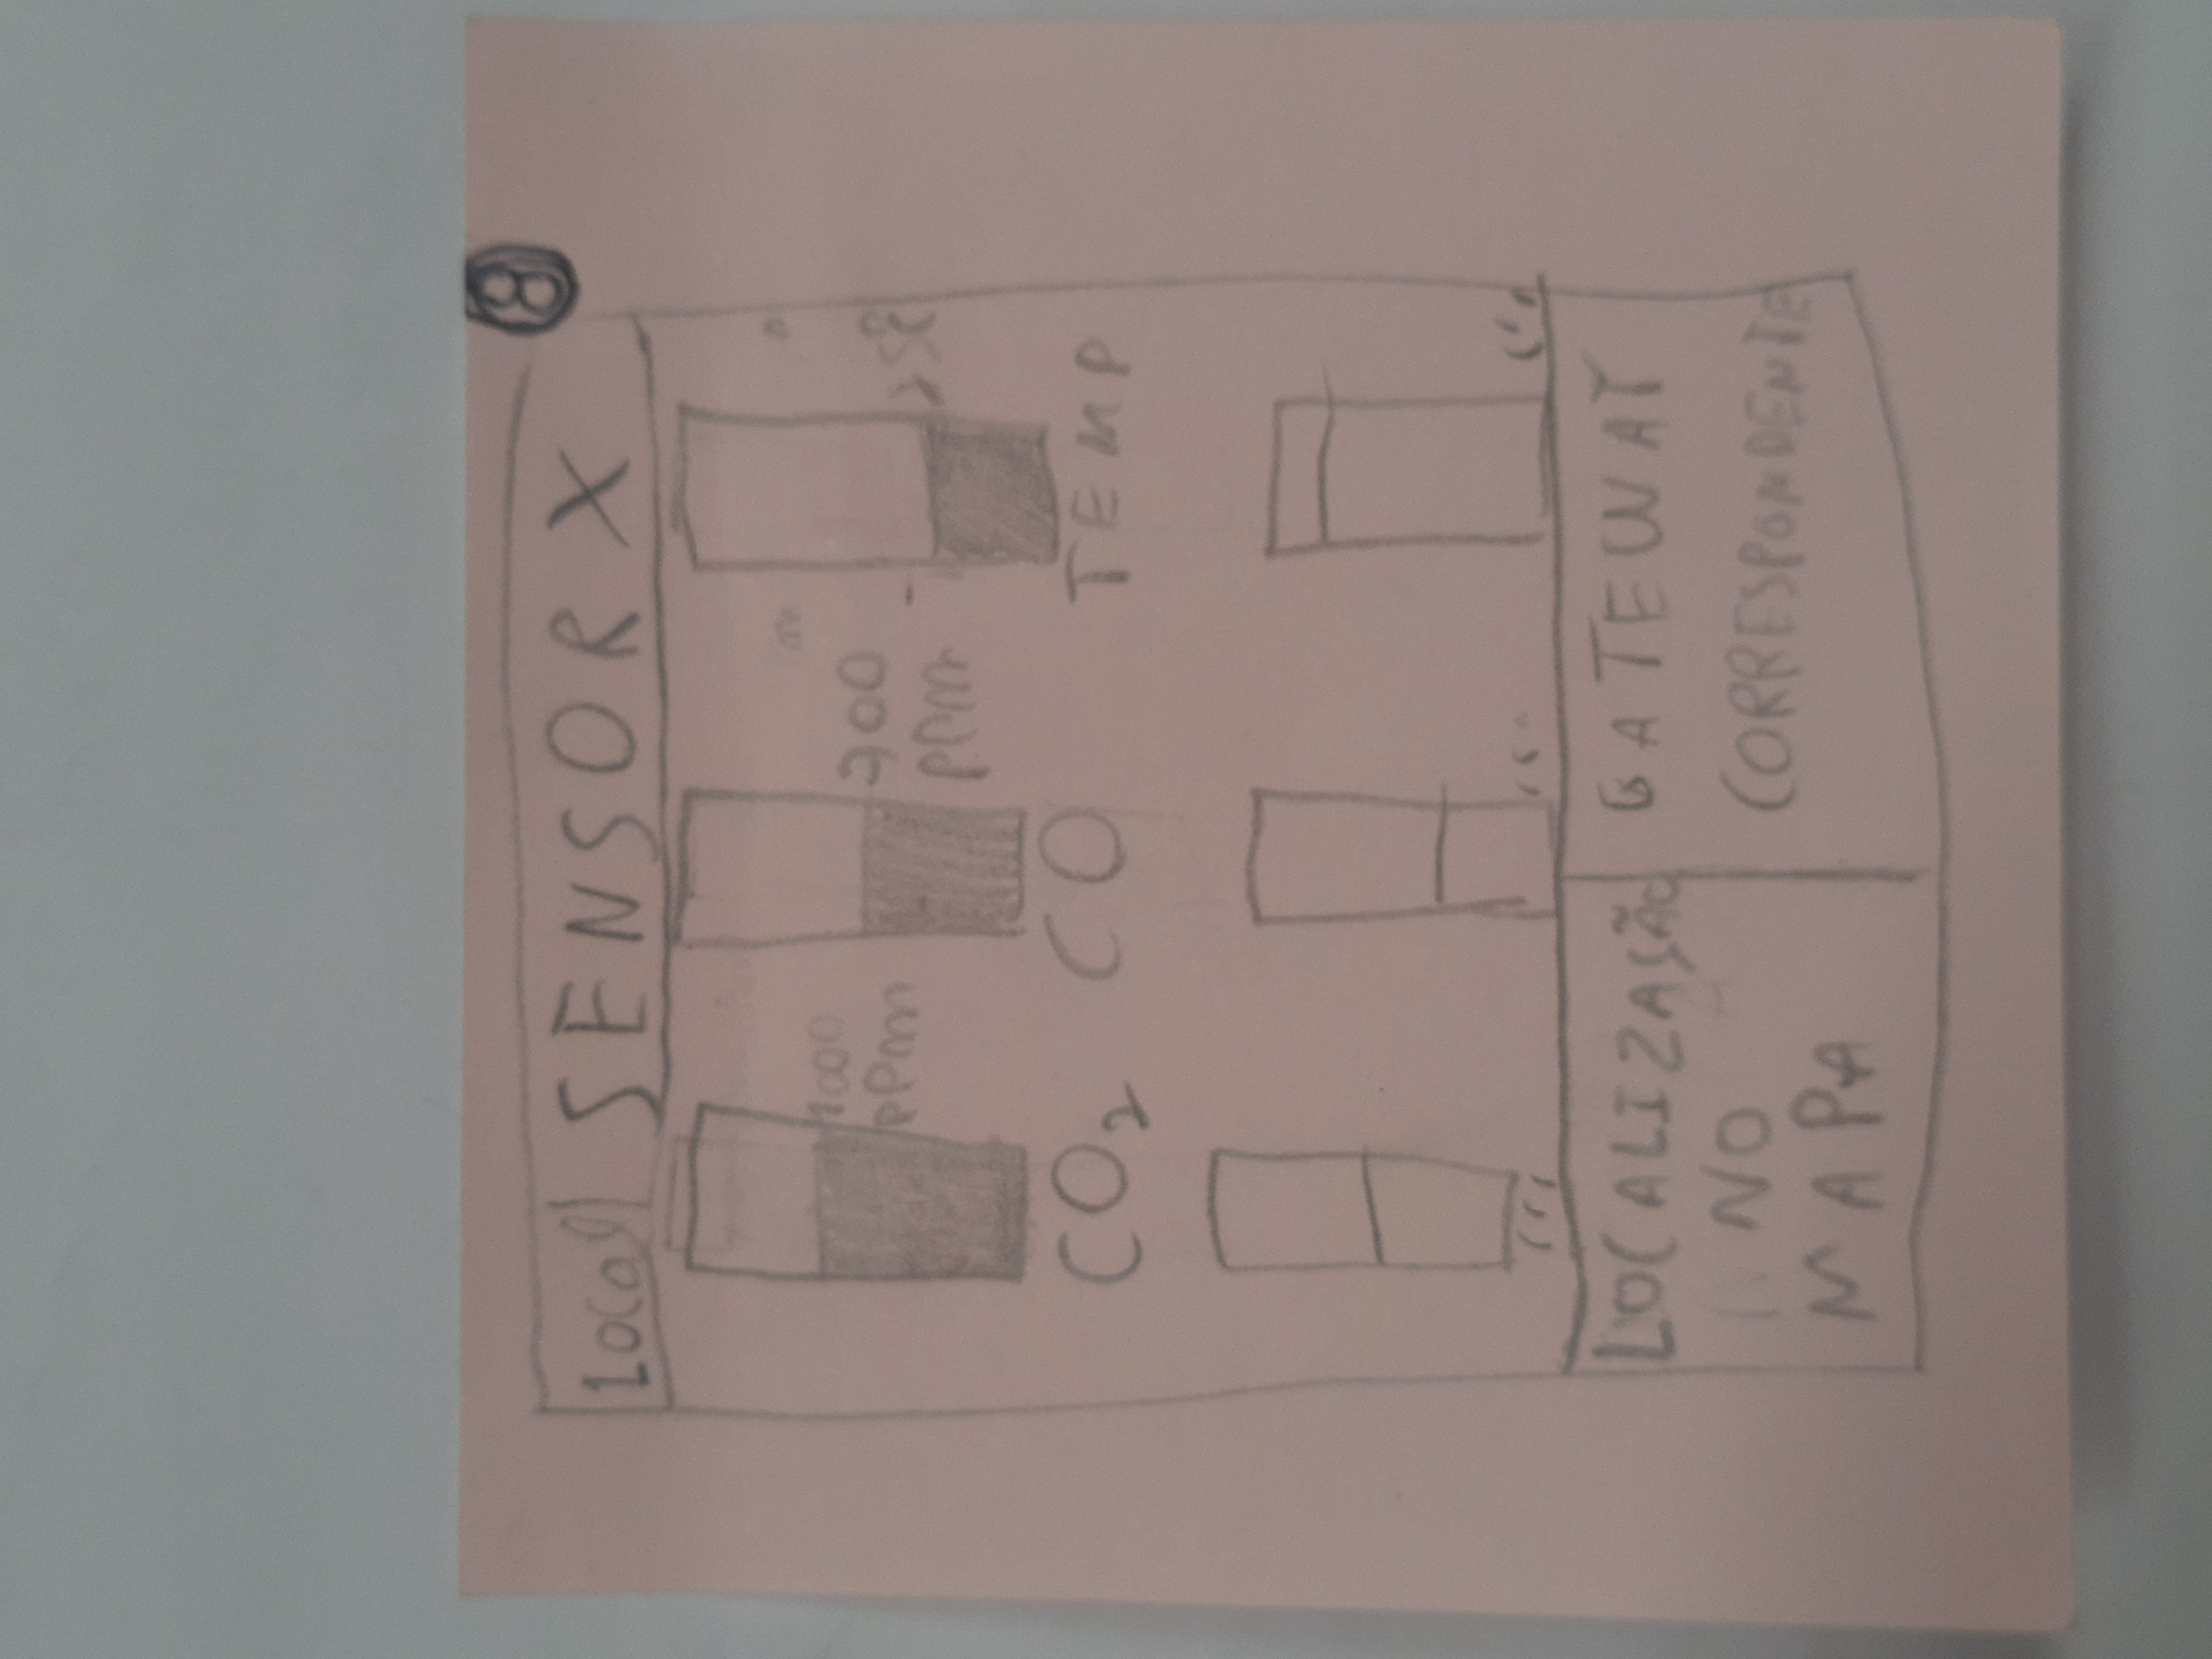
\includegraphics[width=.45\textwidth]{sketches/Situation_8.jpg}
                    \end{turn}\hfill
                }
                \subfloat[Sketch 9]{
                    \begin{turn}{270}
                    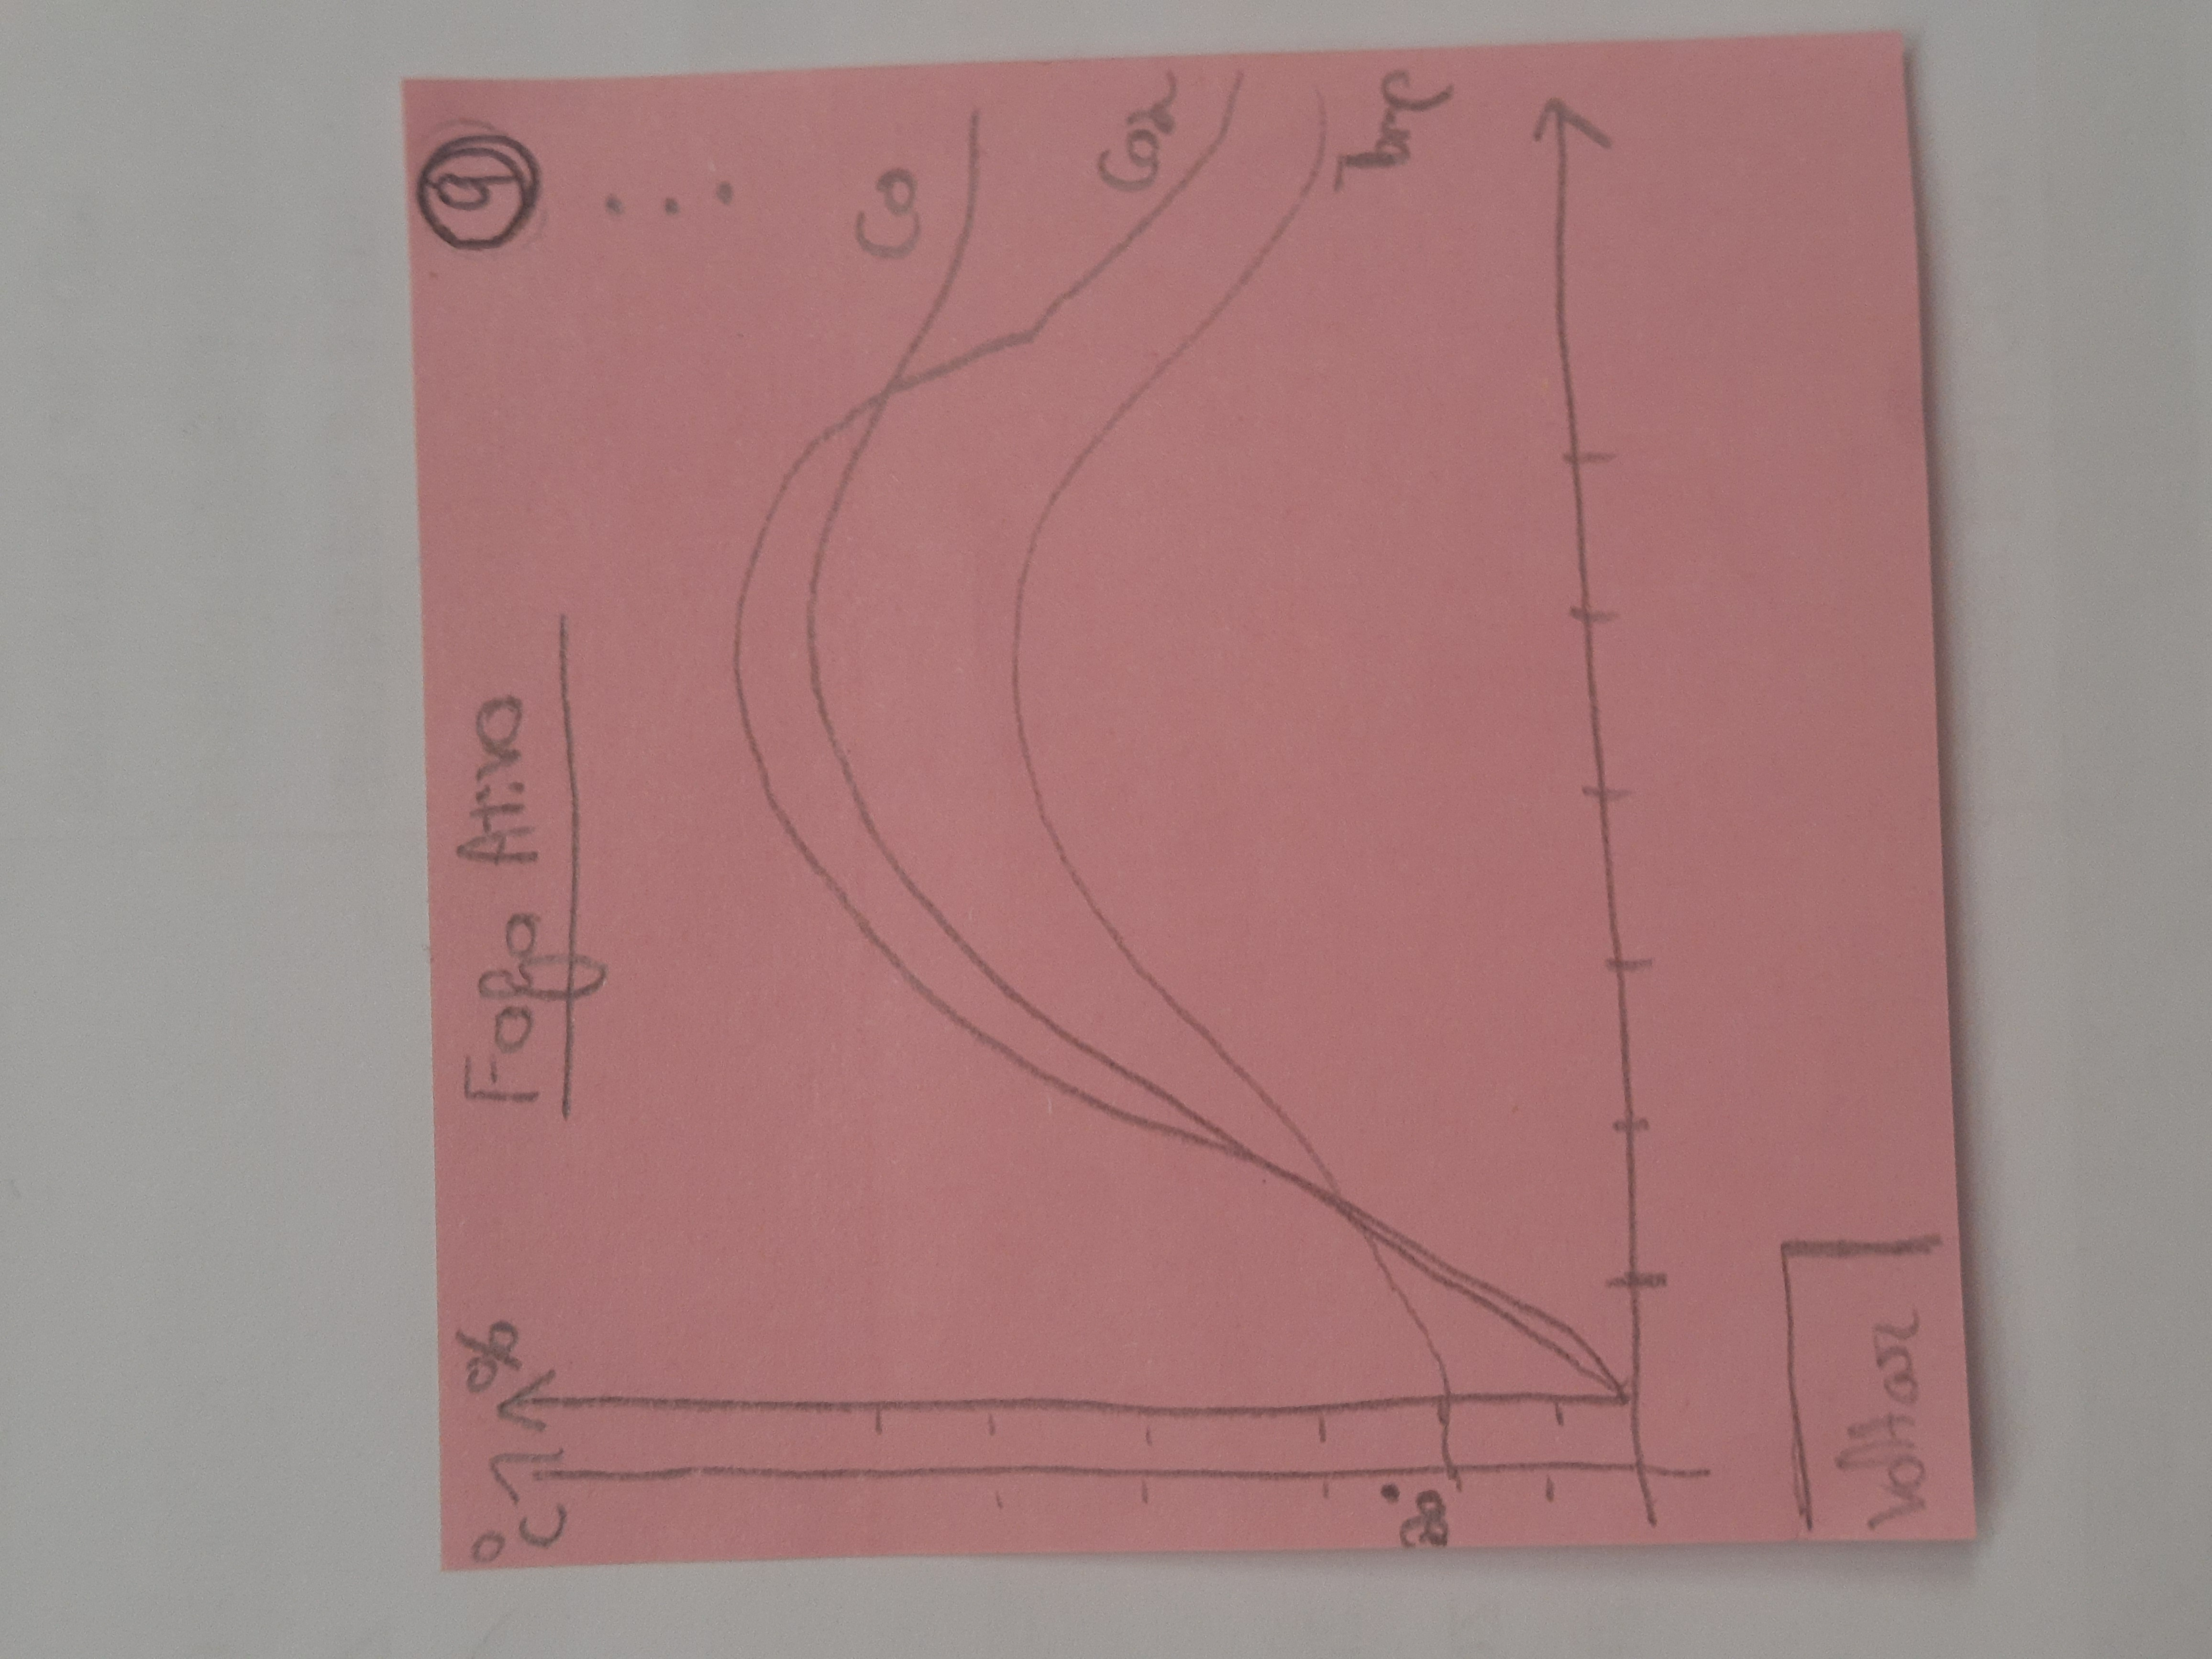
\includegraphics[width=.45\textwidth]{sketches/Situation_9.jpg}
                    \end{turn}
                }%
                    }
                \caption{Single Situation Panel Sketches}
            \end{figure}
        \item Multiple:
            \begin{figure}[H]
                \centerline{%
                \subfloat[Sketch 1]{
                    \begin{turn}{270}
                    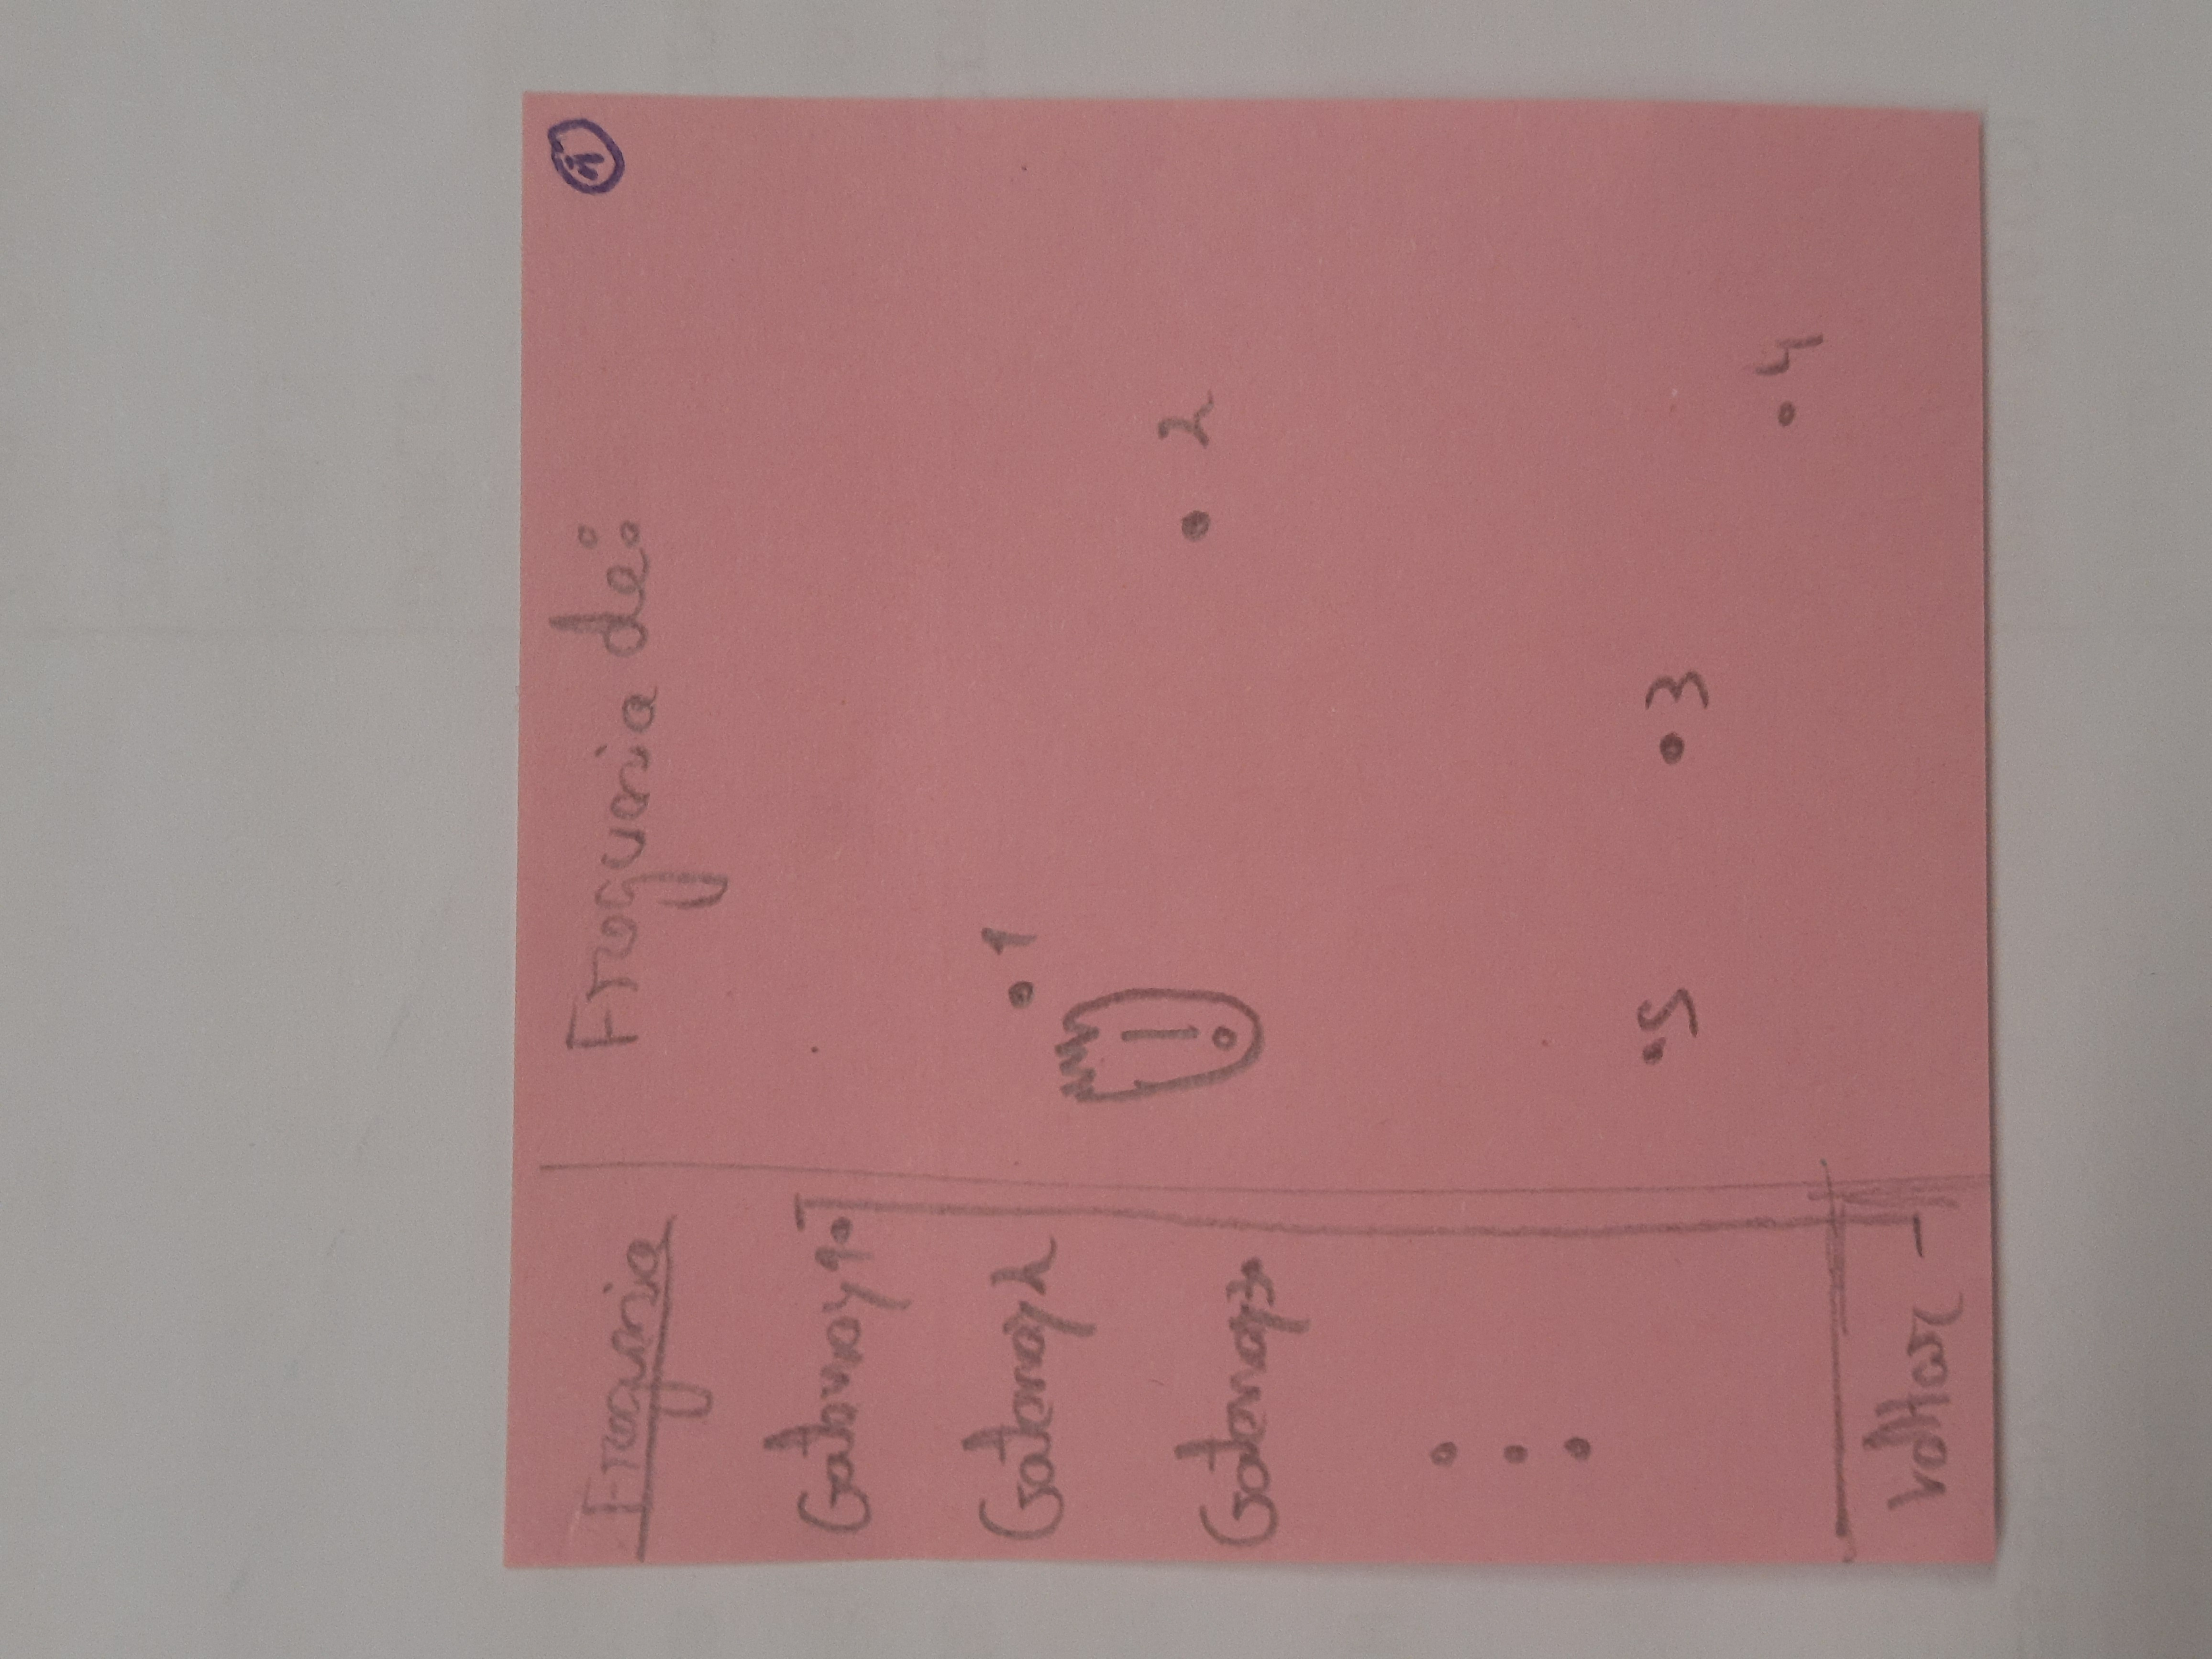
\includegraphics[width=.5\textwidth]{sketches/Situation_mult_1.jpg}
                    \end{turn}
                }\hfill 
                \subfloat[Sketch 2]{
                    \begin{turn}{270}
                    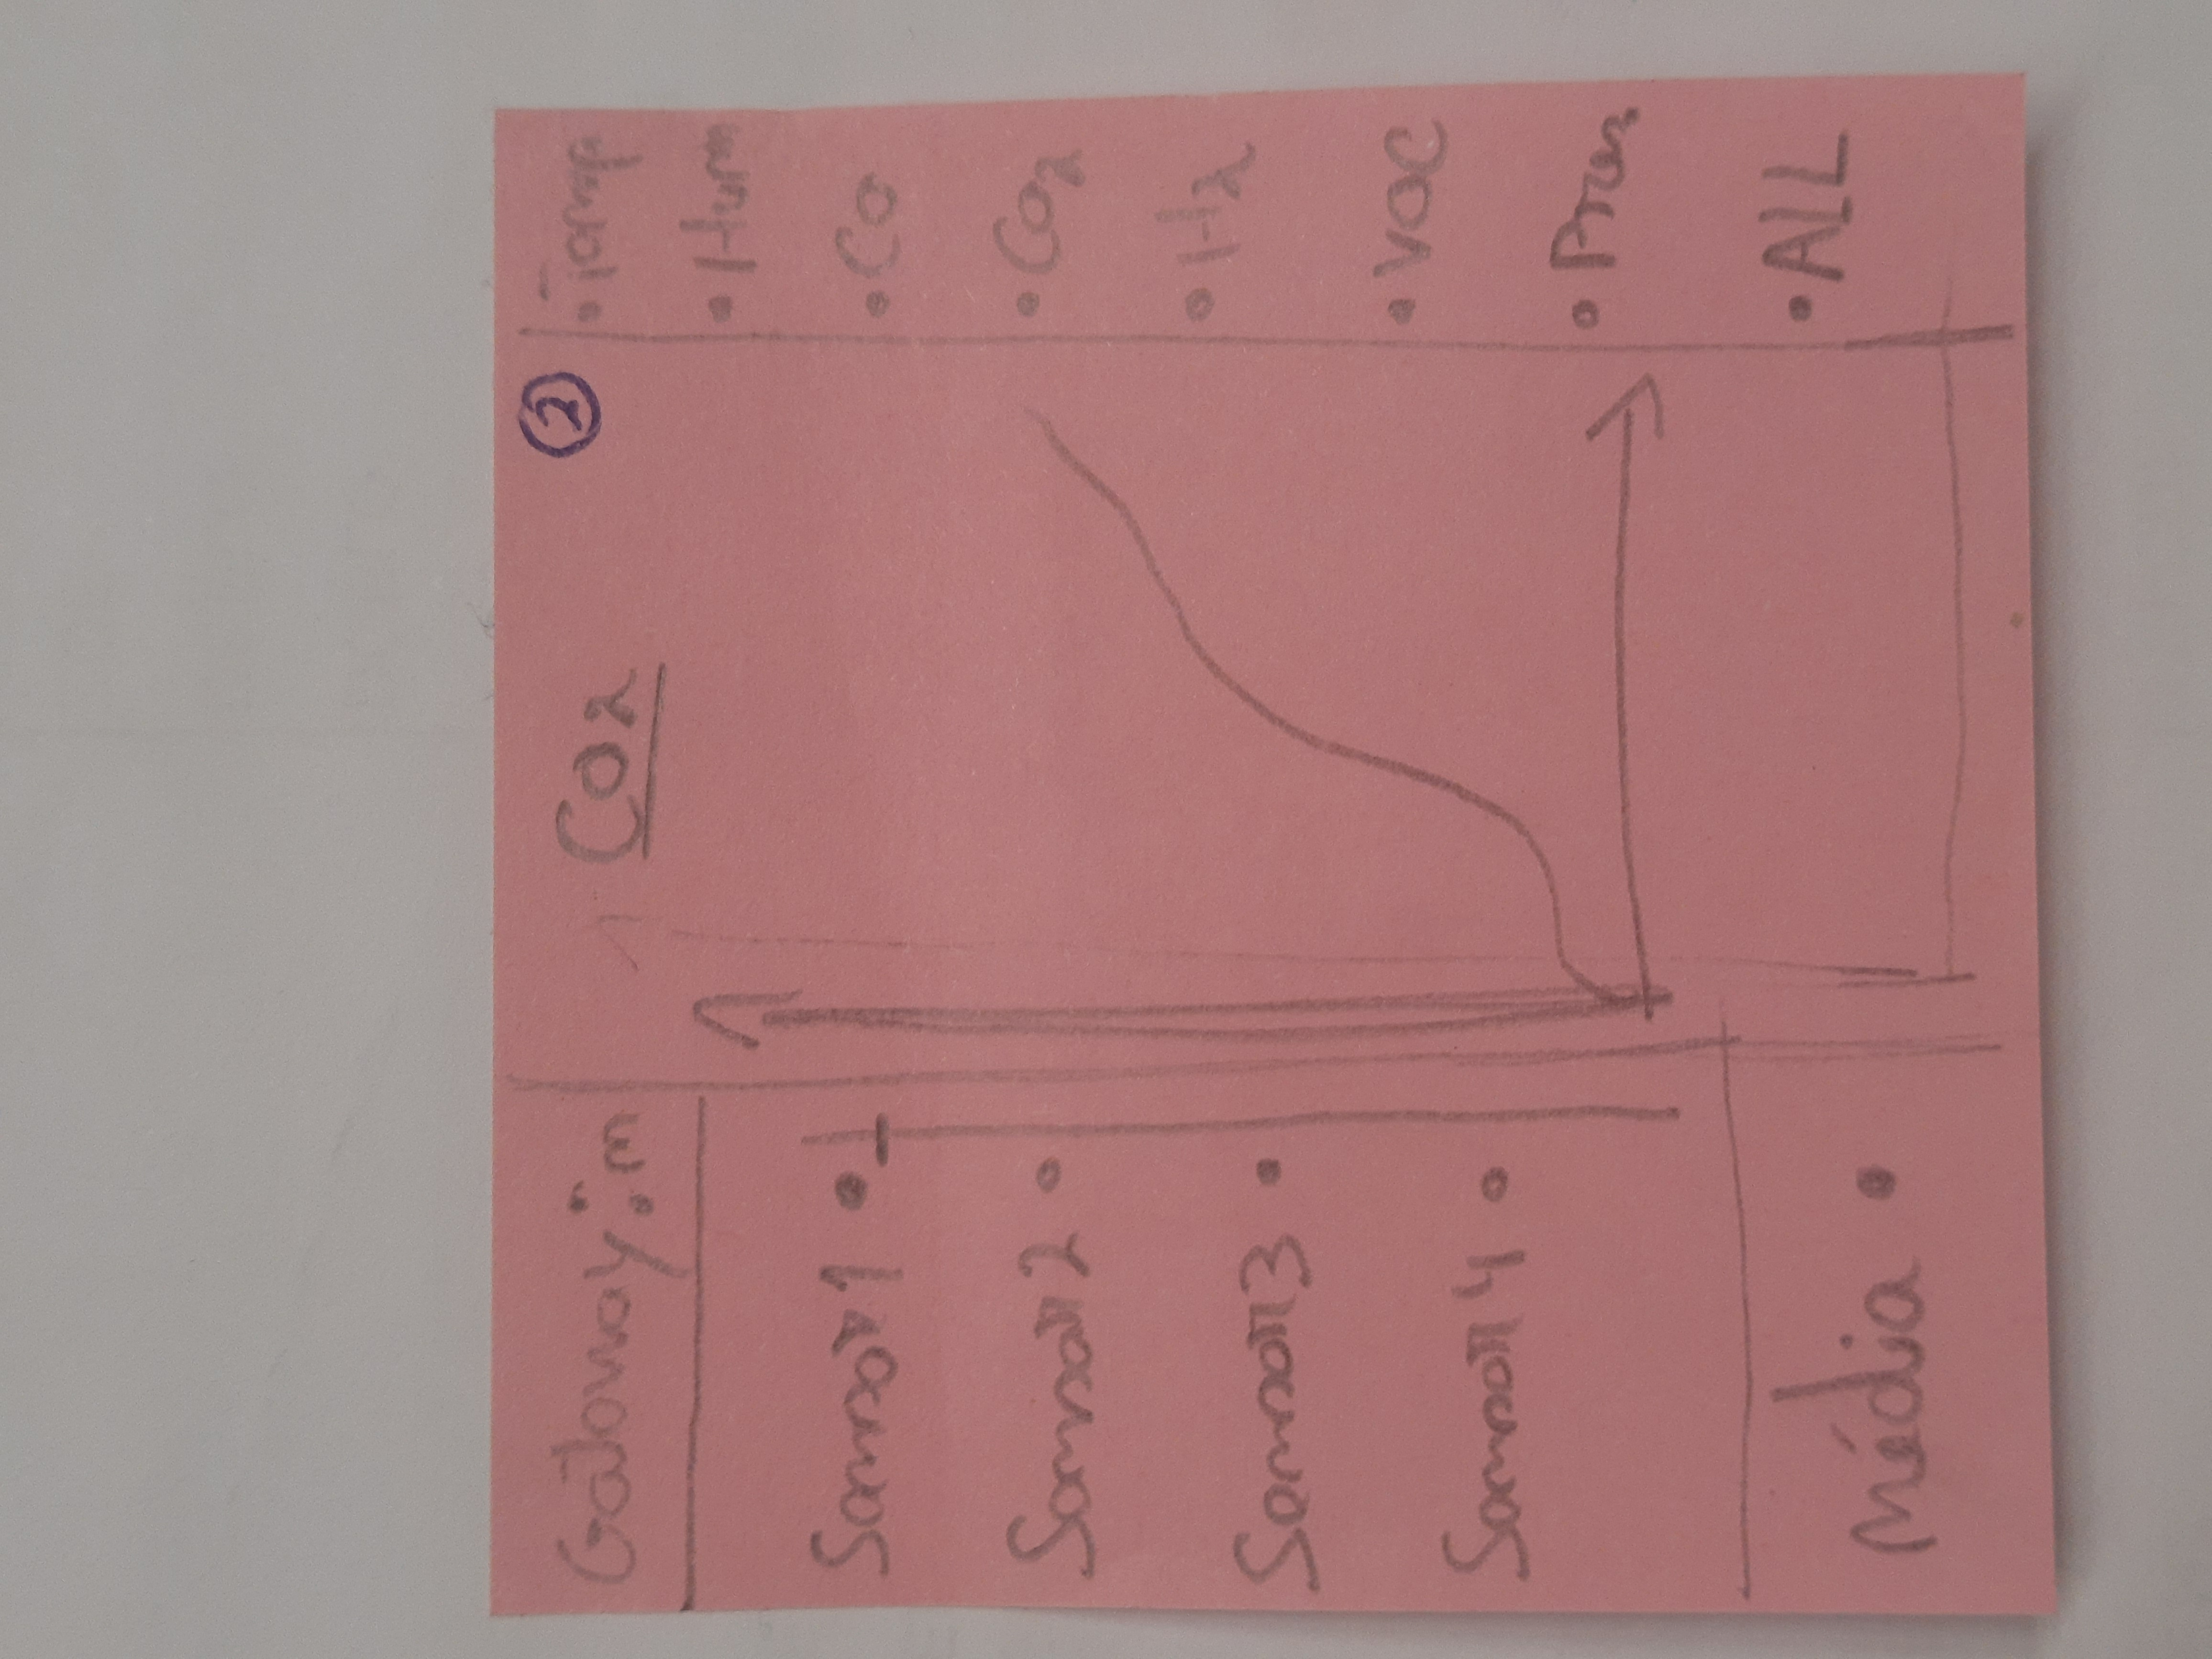
\includegraphics[width=.5\textwidth]{sketches/Situation_mult_2.jpg}
                    \end{turn}
                }\hfill
                \subfloat[Sketch 3]{
                    \begin{turn}{270}
                    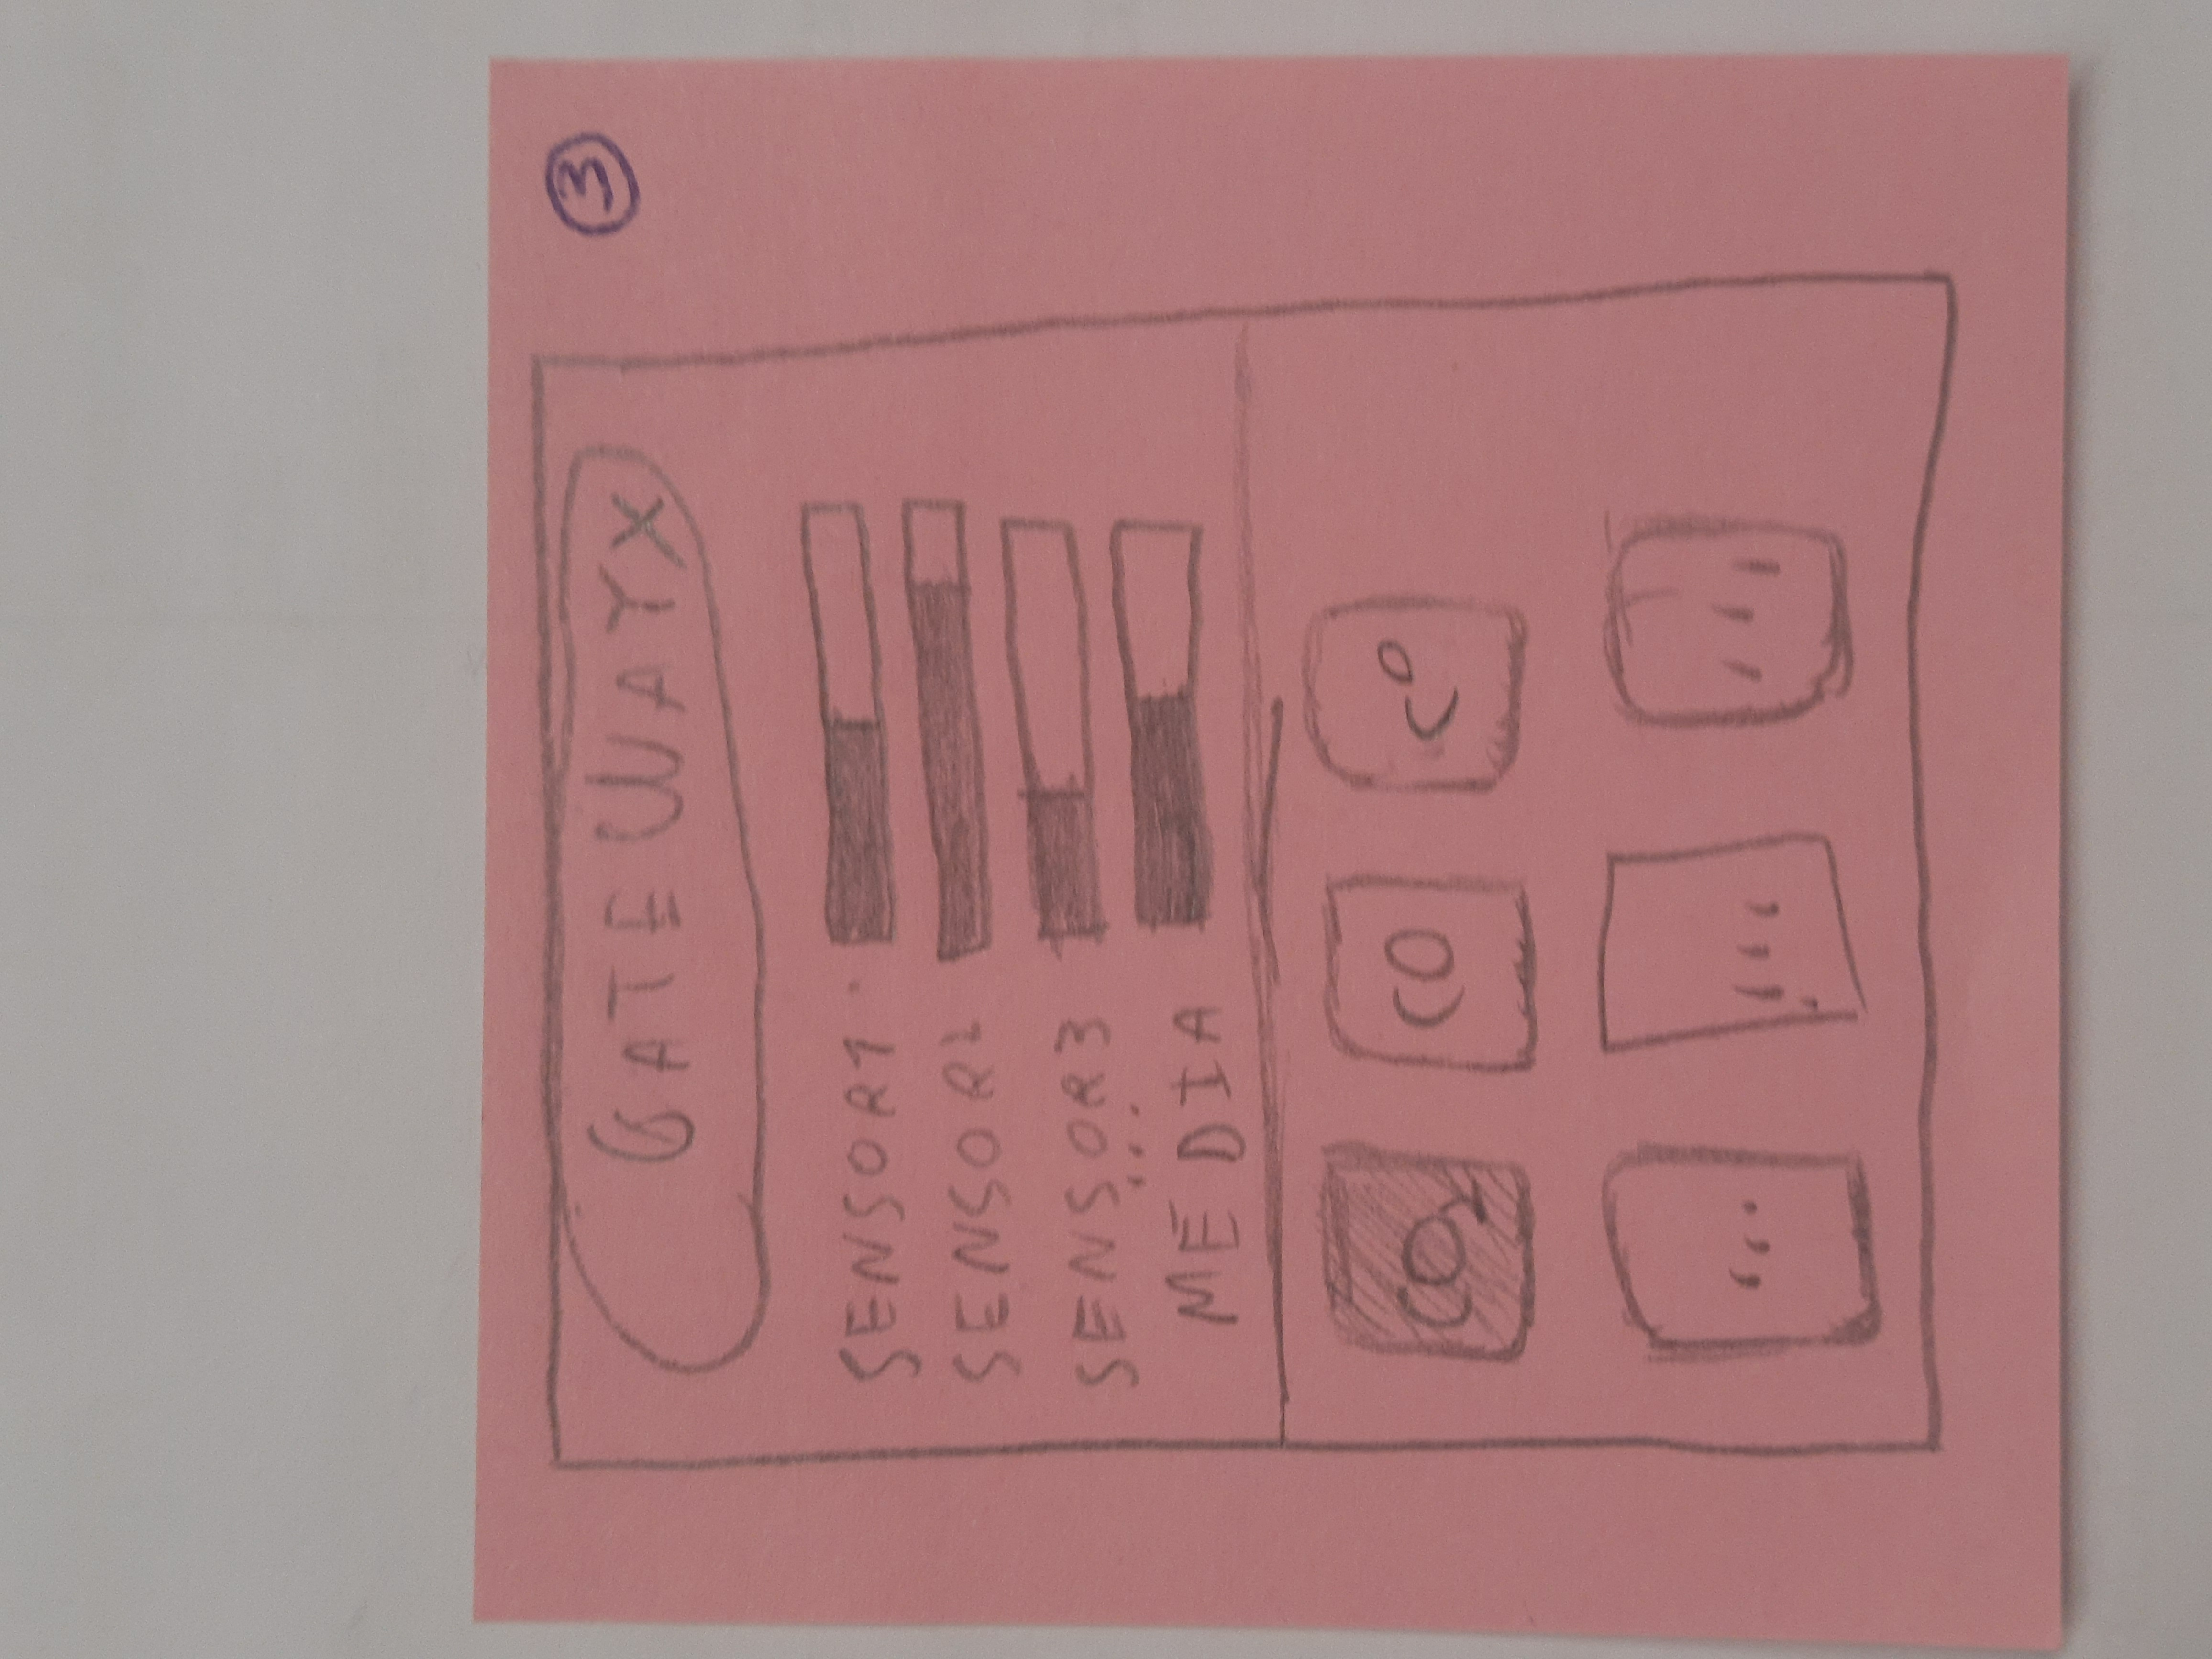
\includegraphics[width=.5\textwidth]{sketches/Situation_mult_3.jpg}
                    \end{turn}
                }%
                }
                \centerline{%
                \subfloat[Sketch 4]{
                    \begin{turn}{270}
                    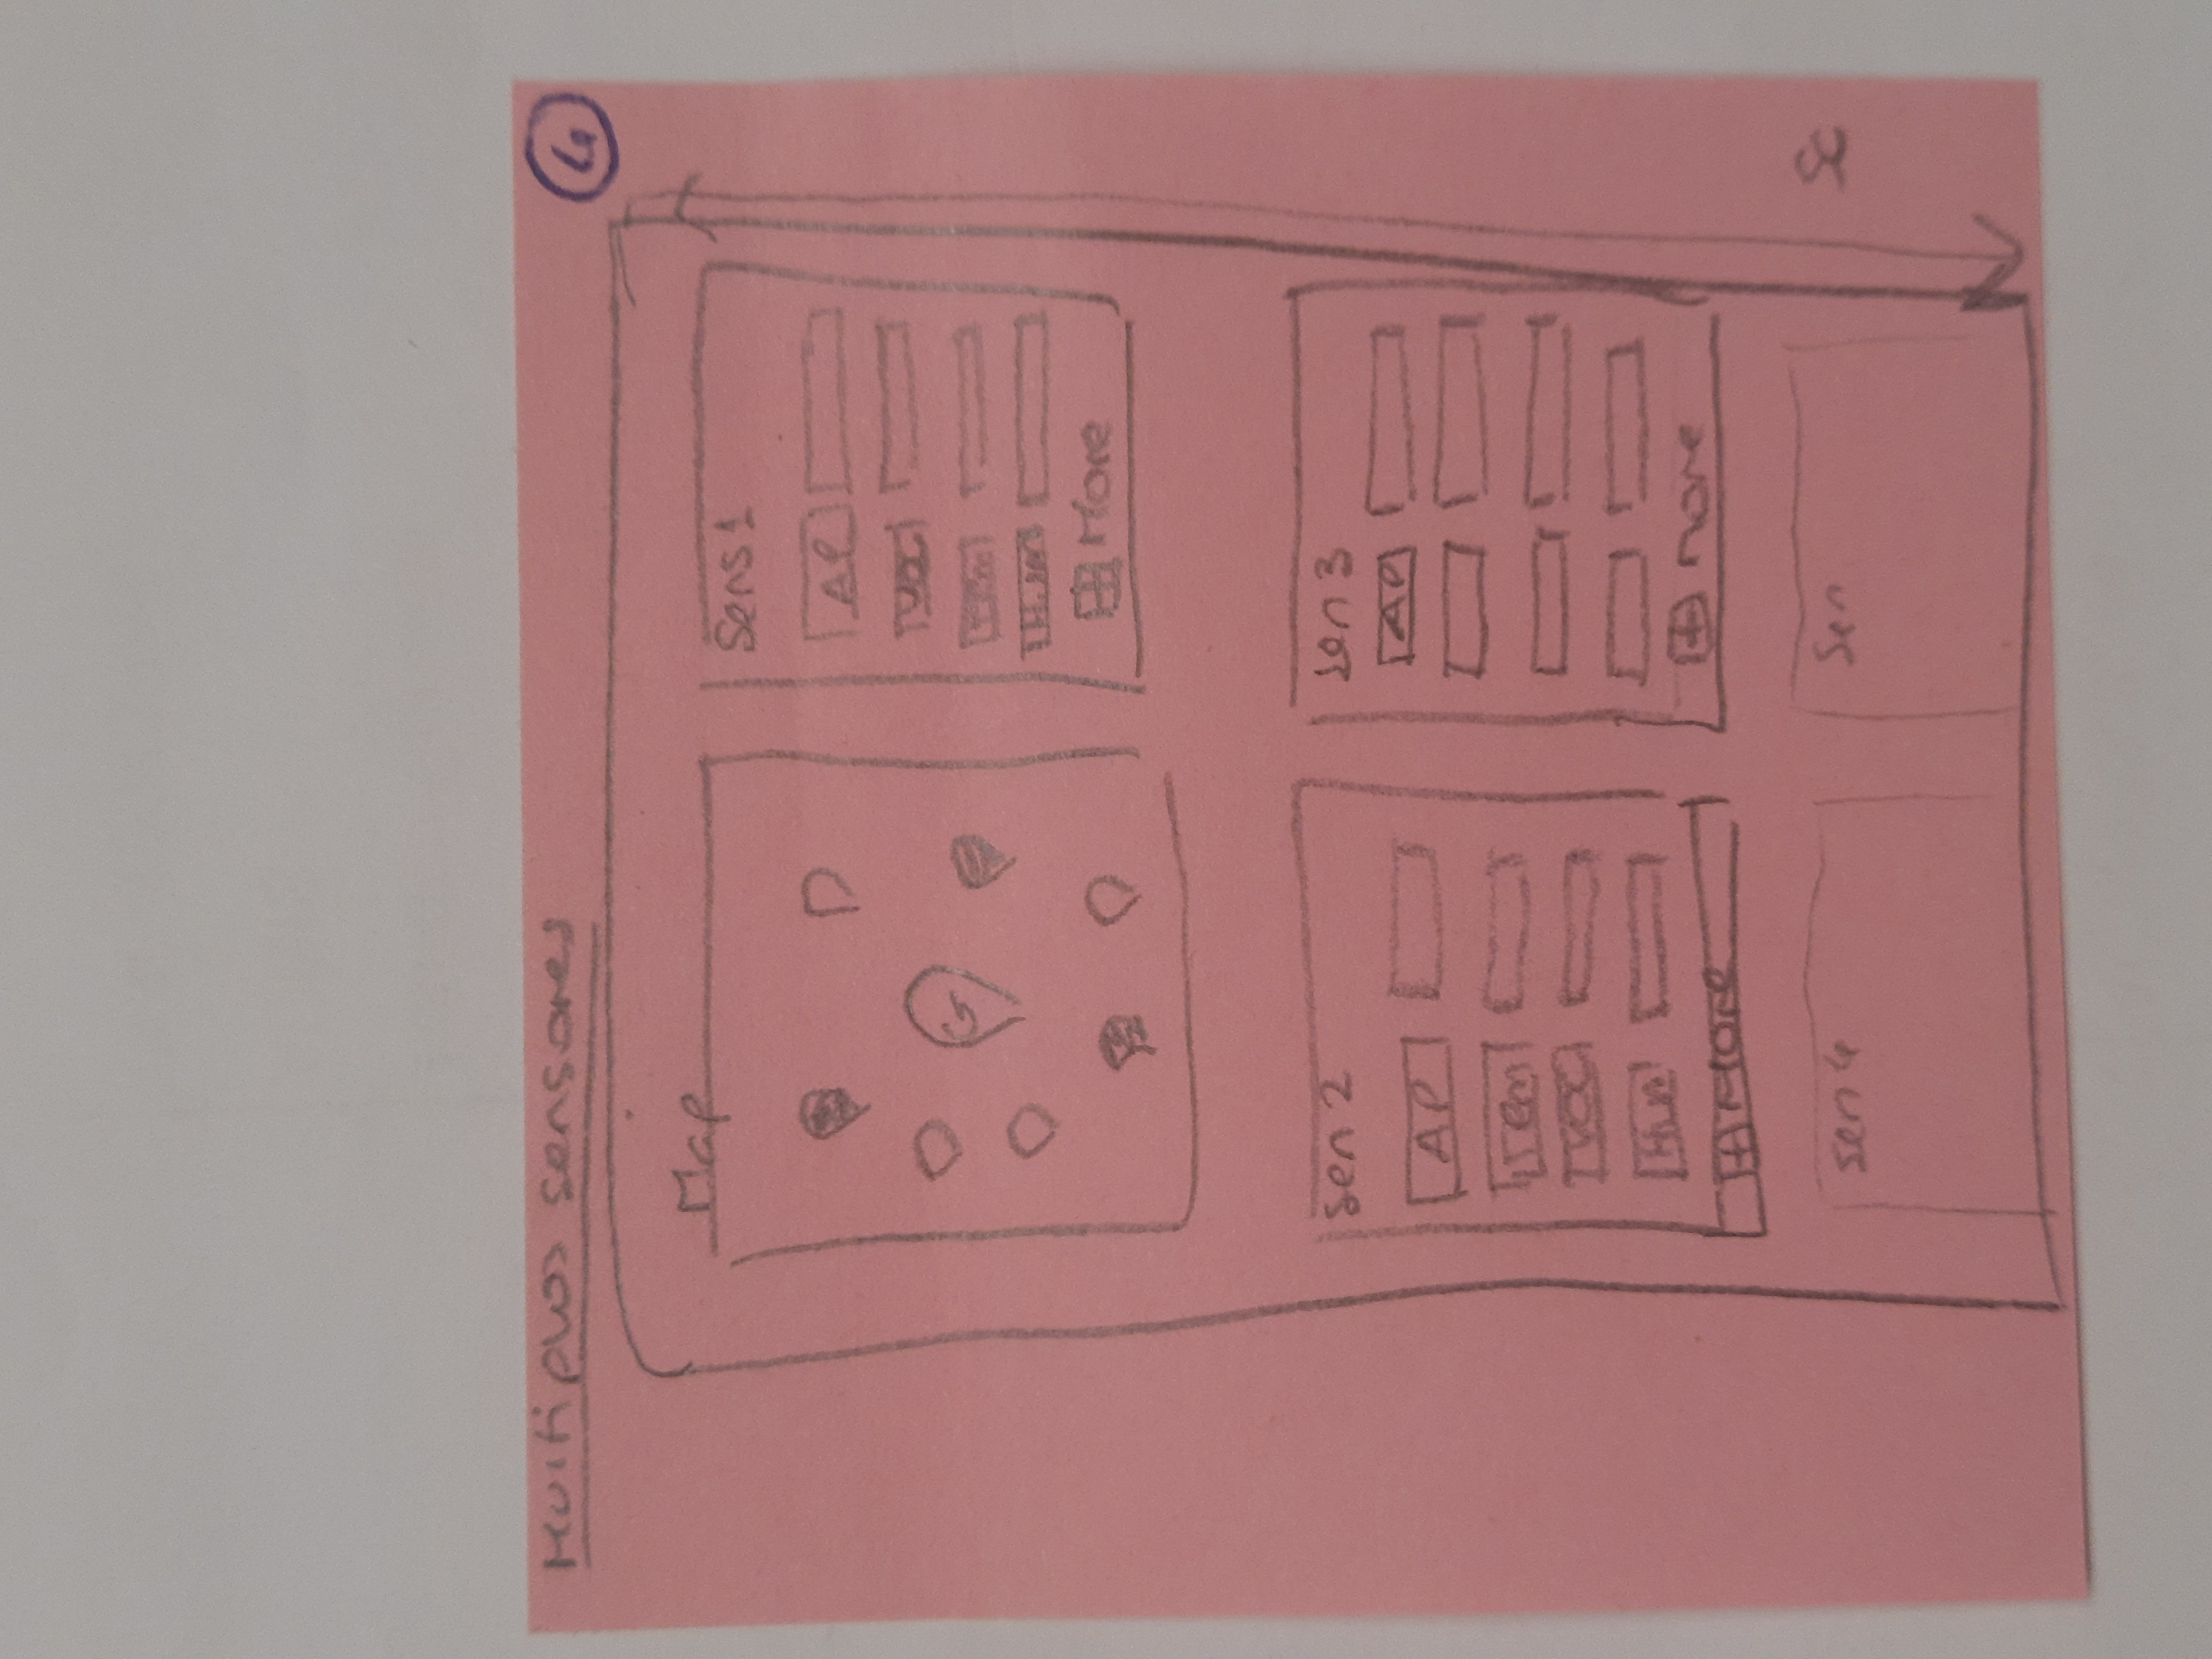
\includegraphics[width=.5\textwidth]{sketches/Situation_mult_4.jpg}
                    \end{turn}
                }\hfill
                \subfloat[Sketch 5]{
                    \begin{turn}{270}
                    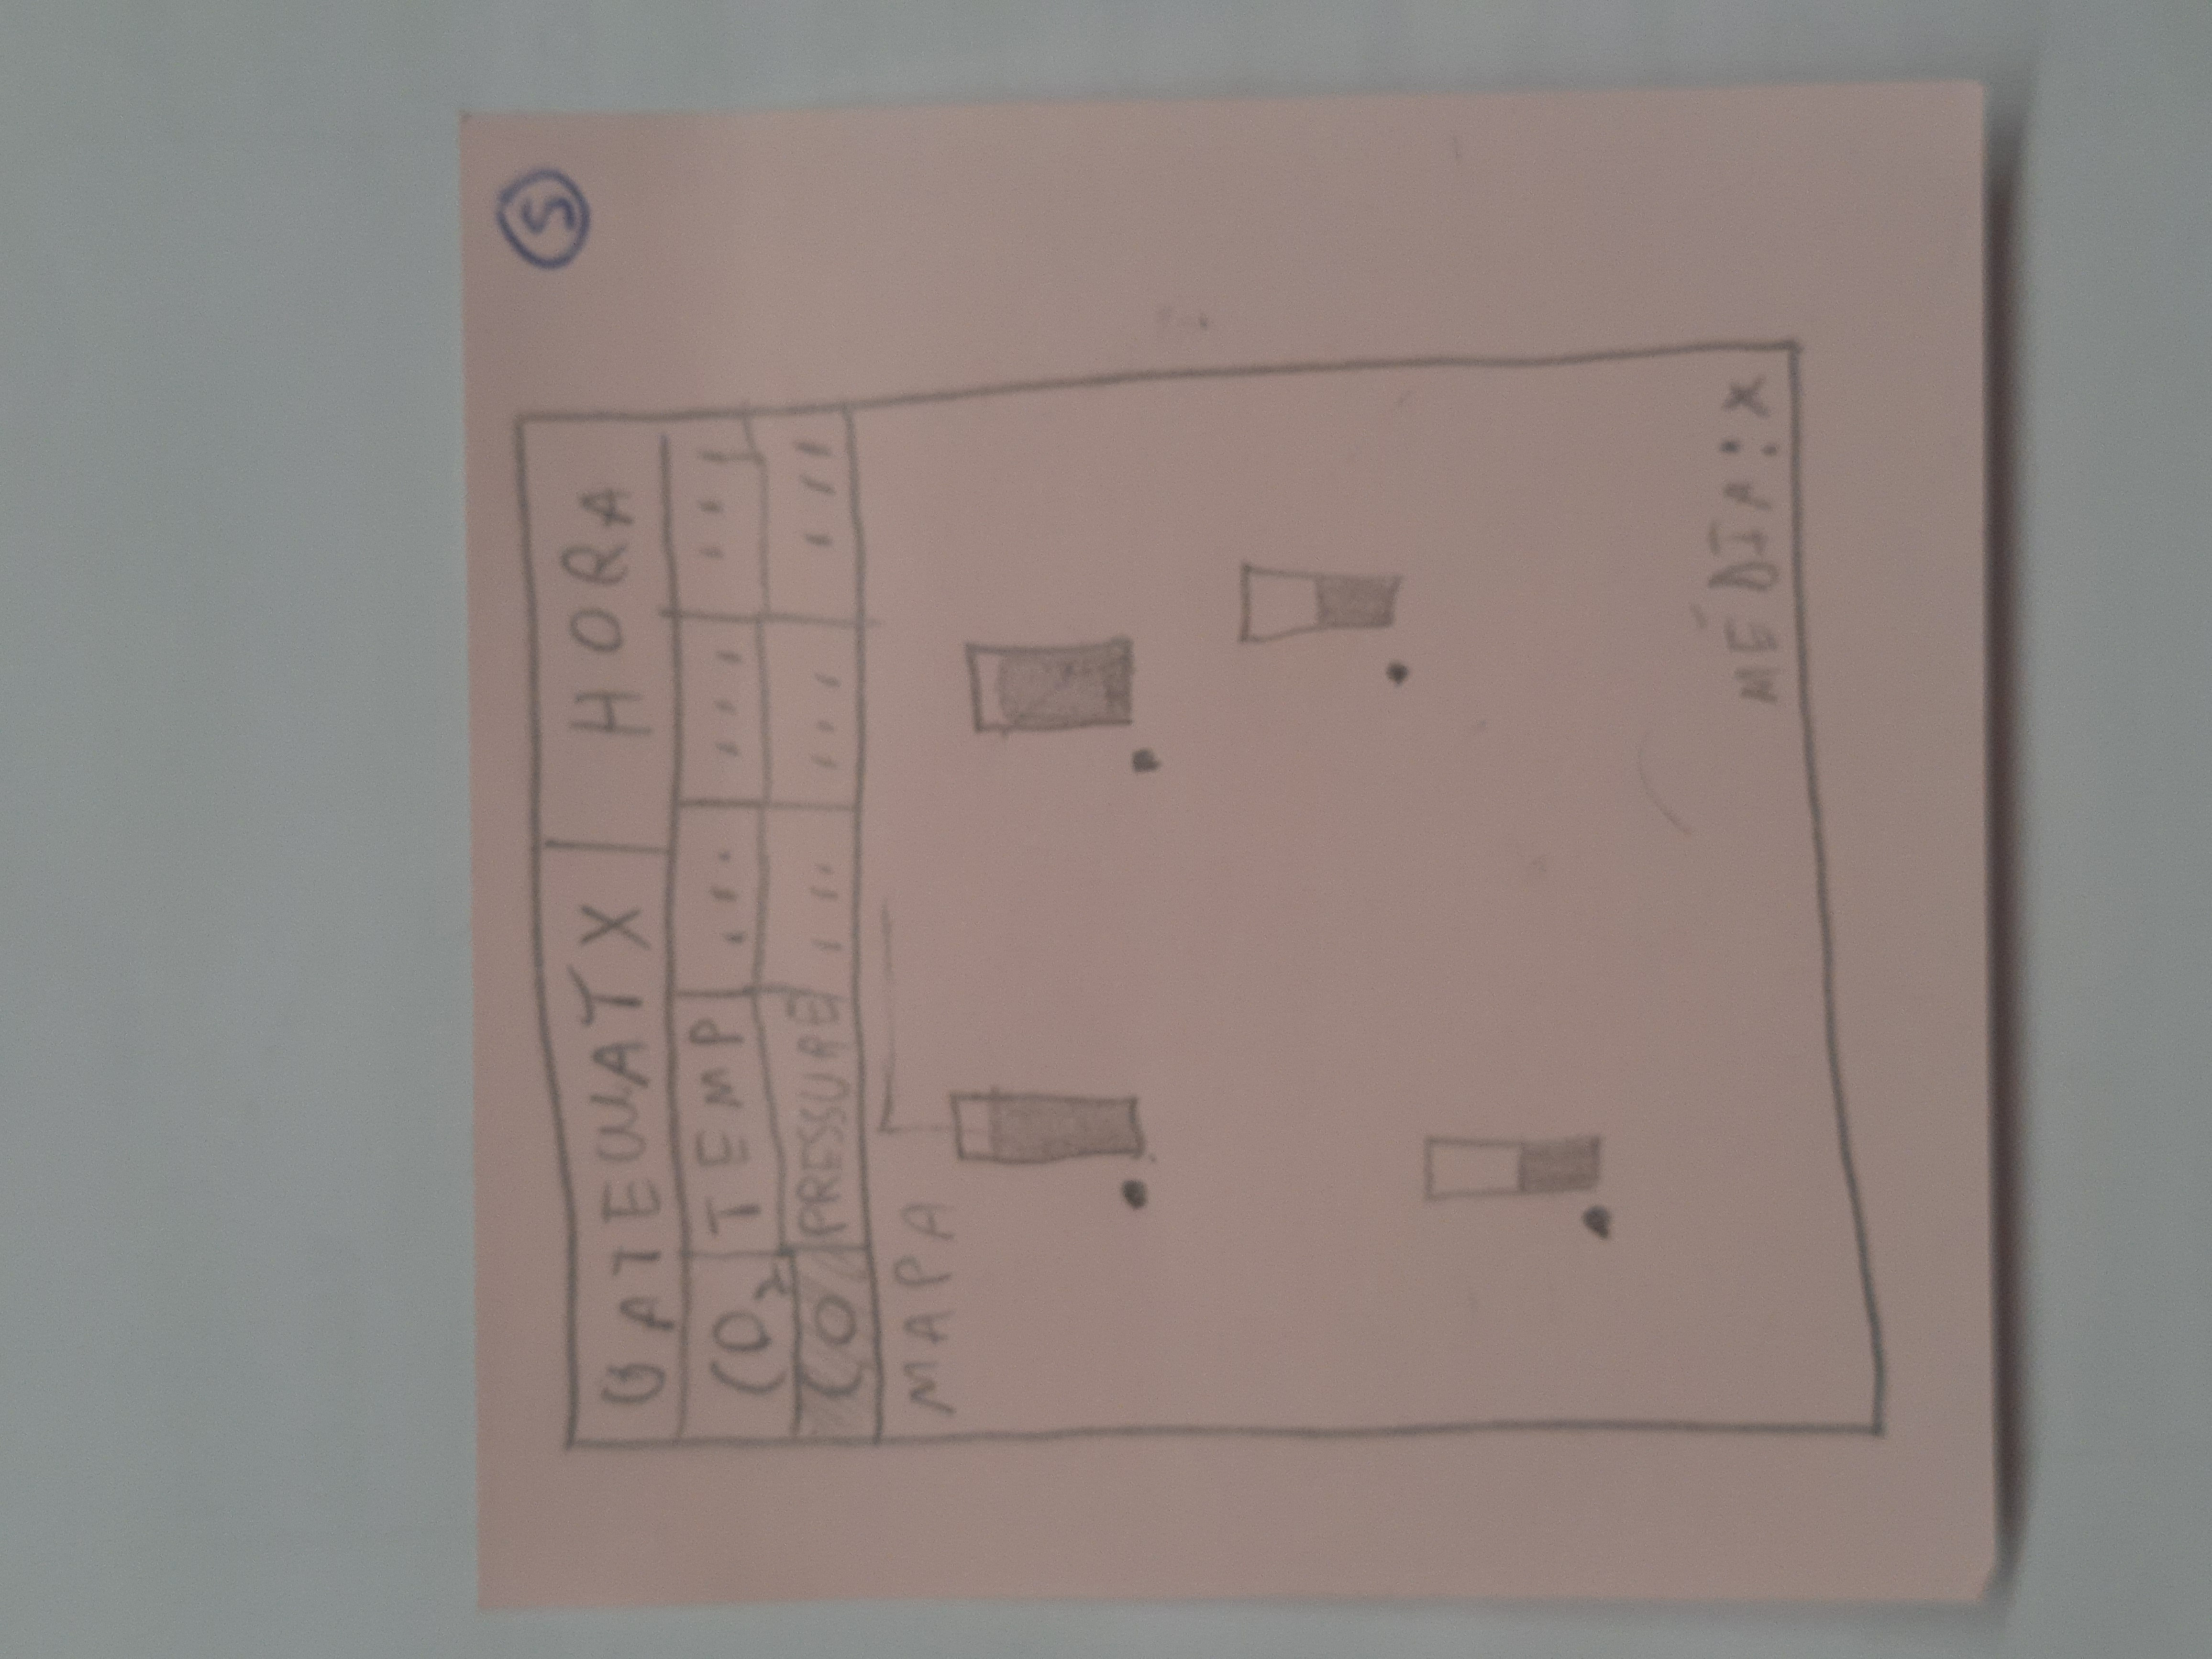
\includegraphics[width=.5\textwidth]{sketches/Situation_mult_5.jpg}
                    \end{turn}
                }\hfill
                \subfloat[Sketch 6]{
                    \begin{turn}{270}
                    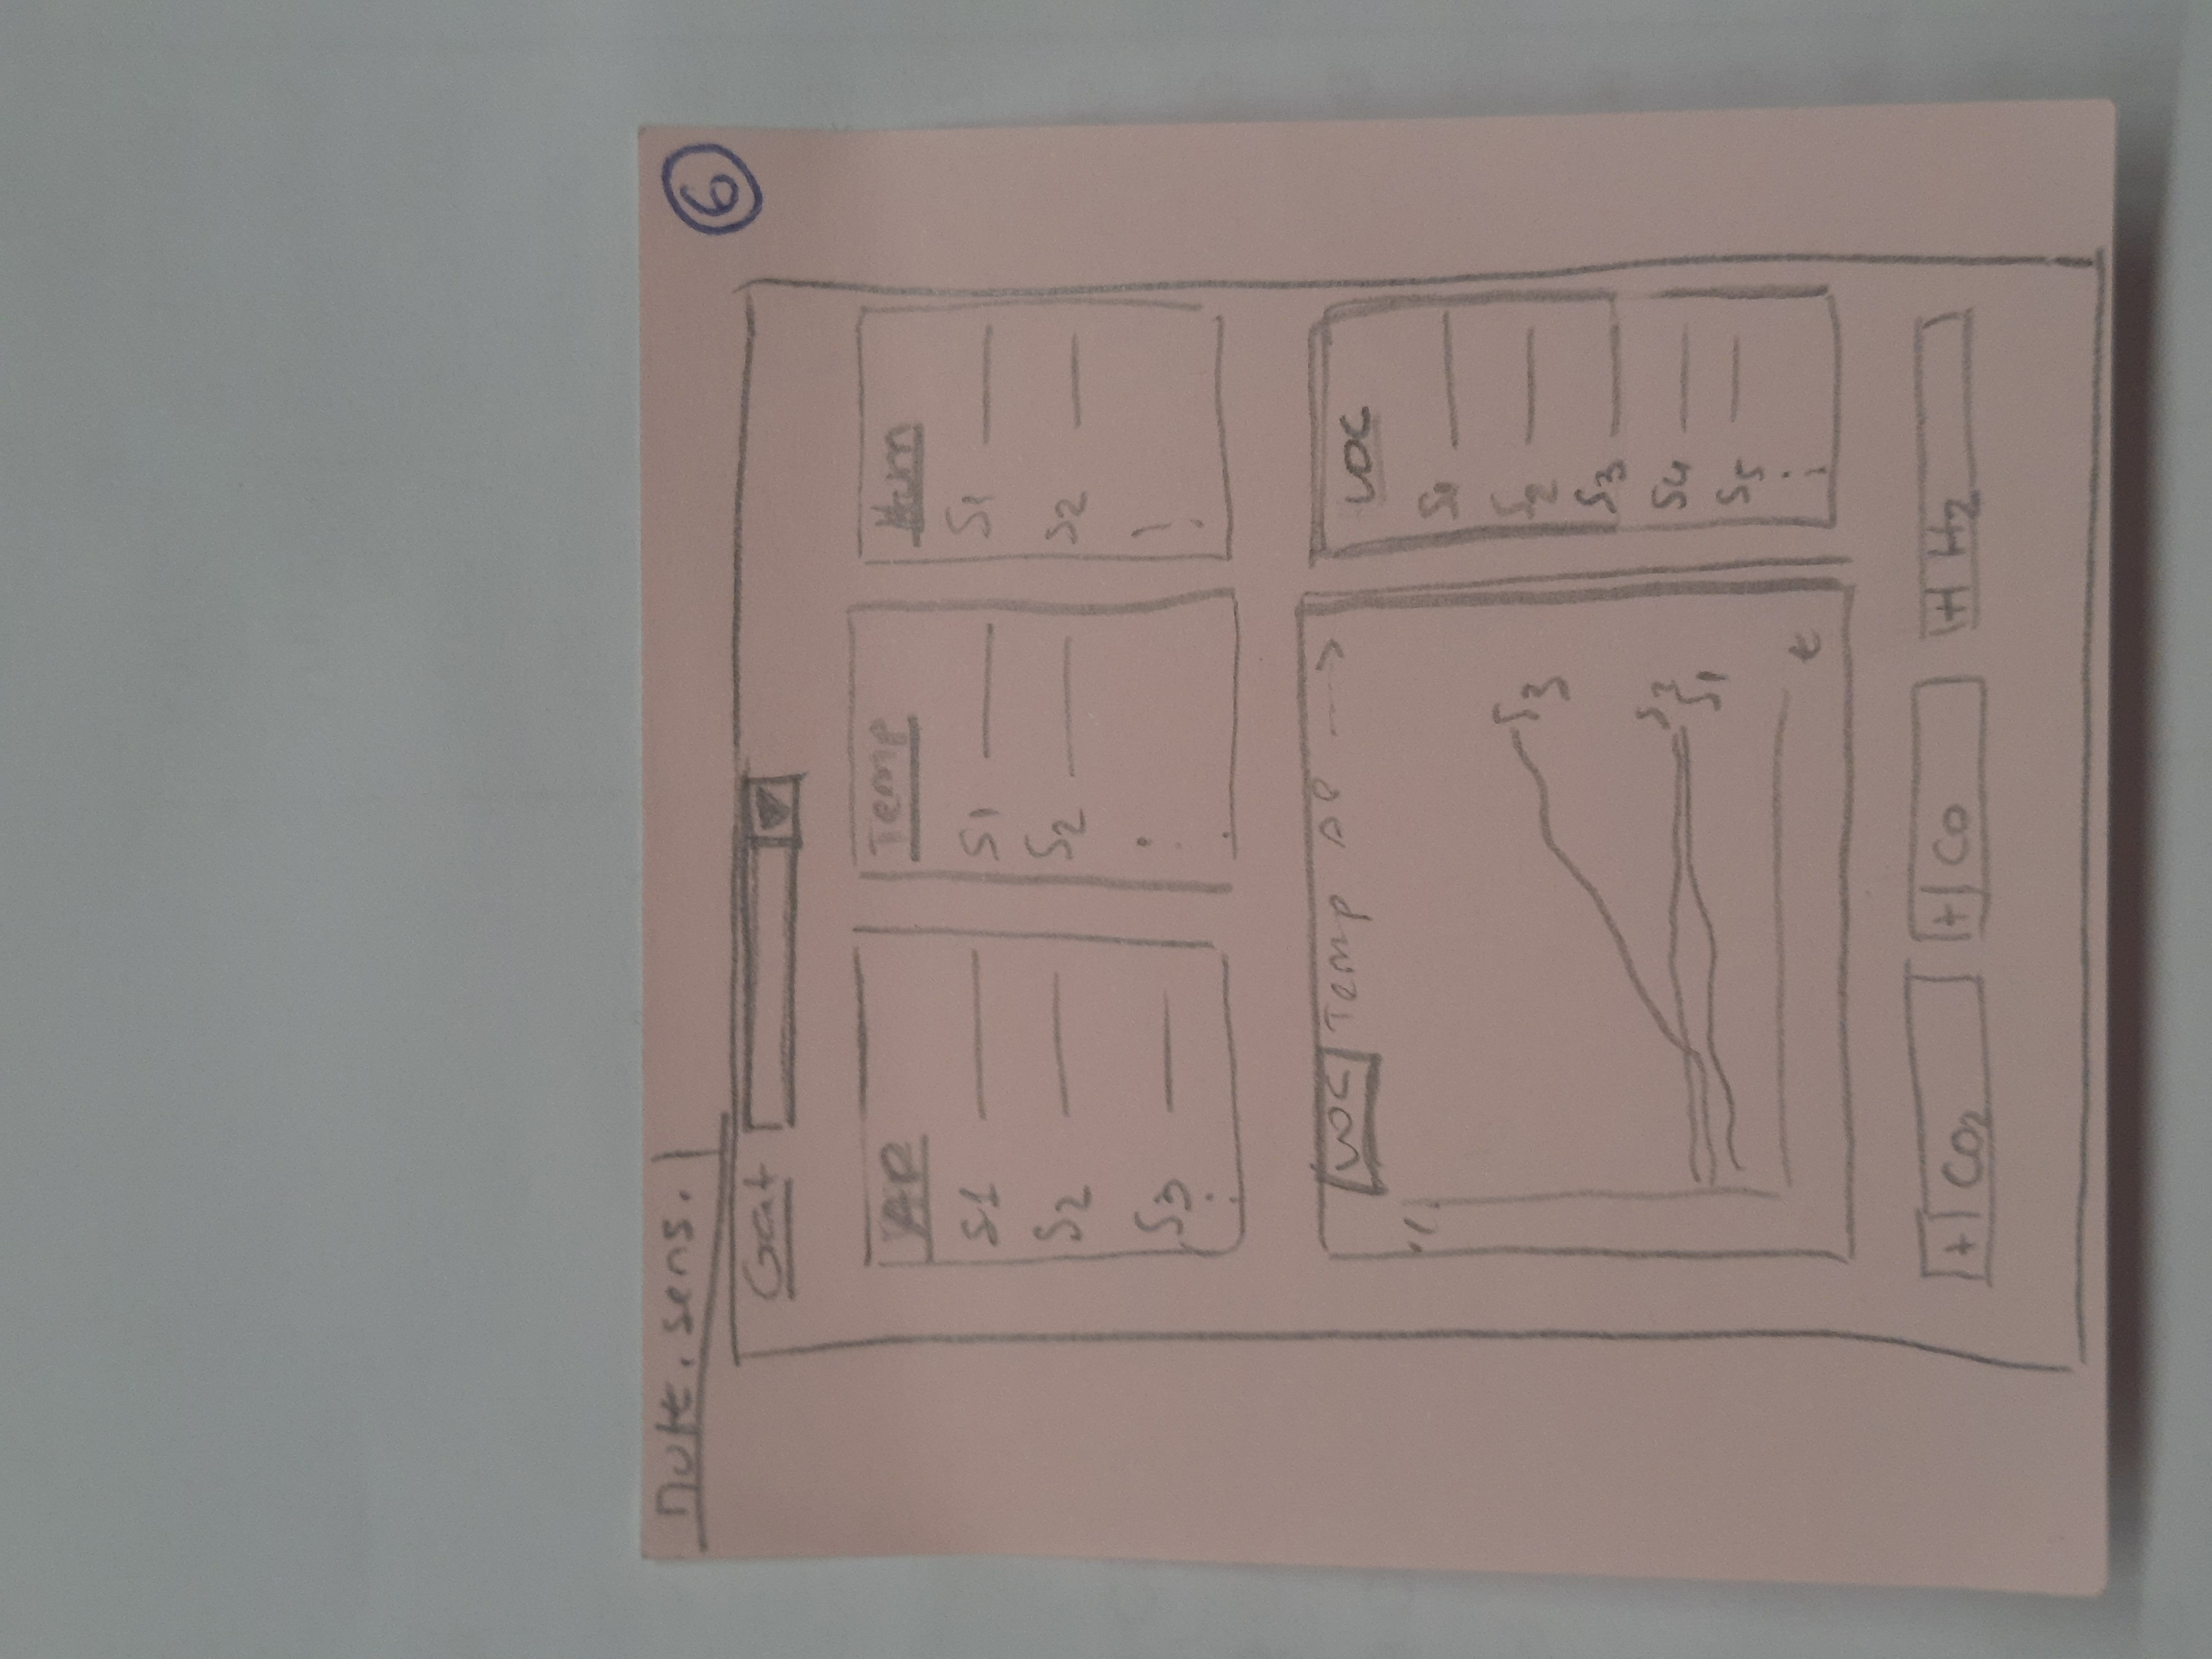
\includegraphics[width=.5\textwidth]{sketches/Situation_mult_6.jpg}
                    \end{turn}
                }%
                }
            \caption{Multiple Situation Panel Sketches}
            \end{figure}
        \end{itemize}
    \item \textbf{Camera Panel:}
        \begin{figure}[H]
            \centerline{%
            \subfloat[Sketch 1]{
                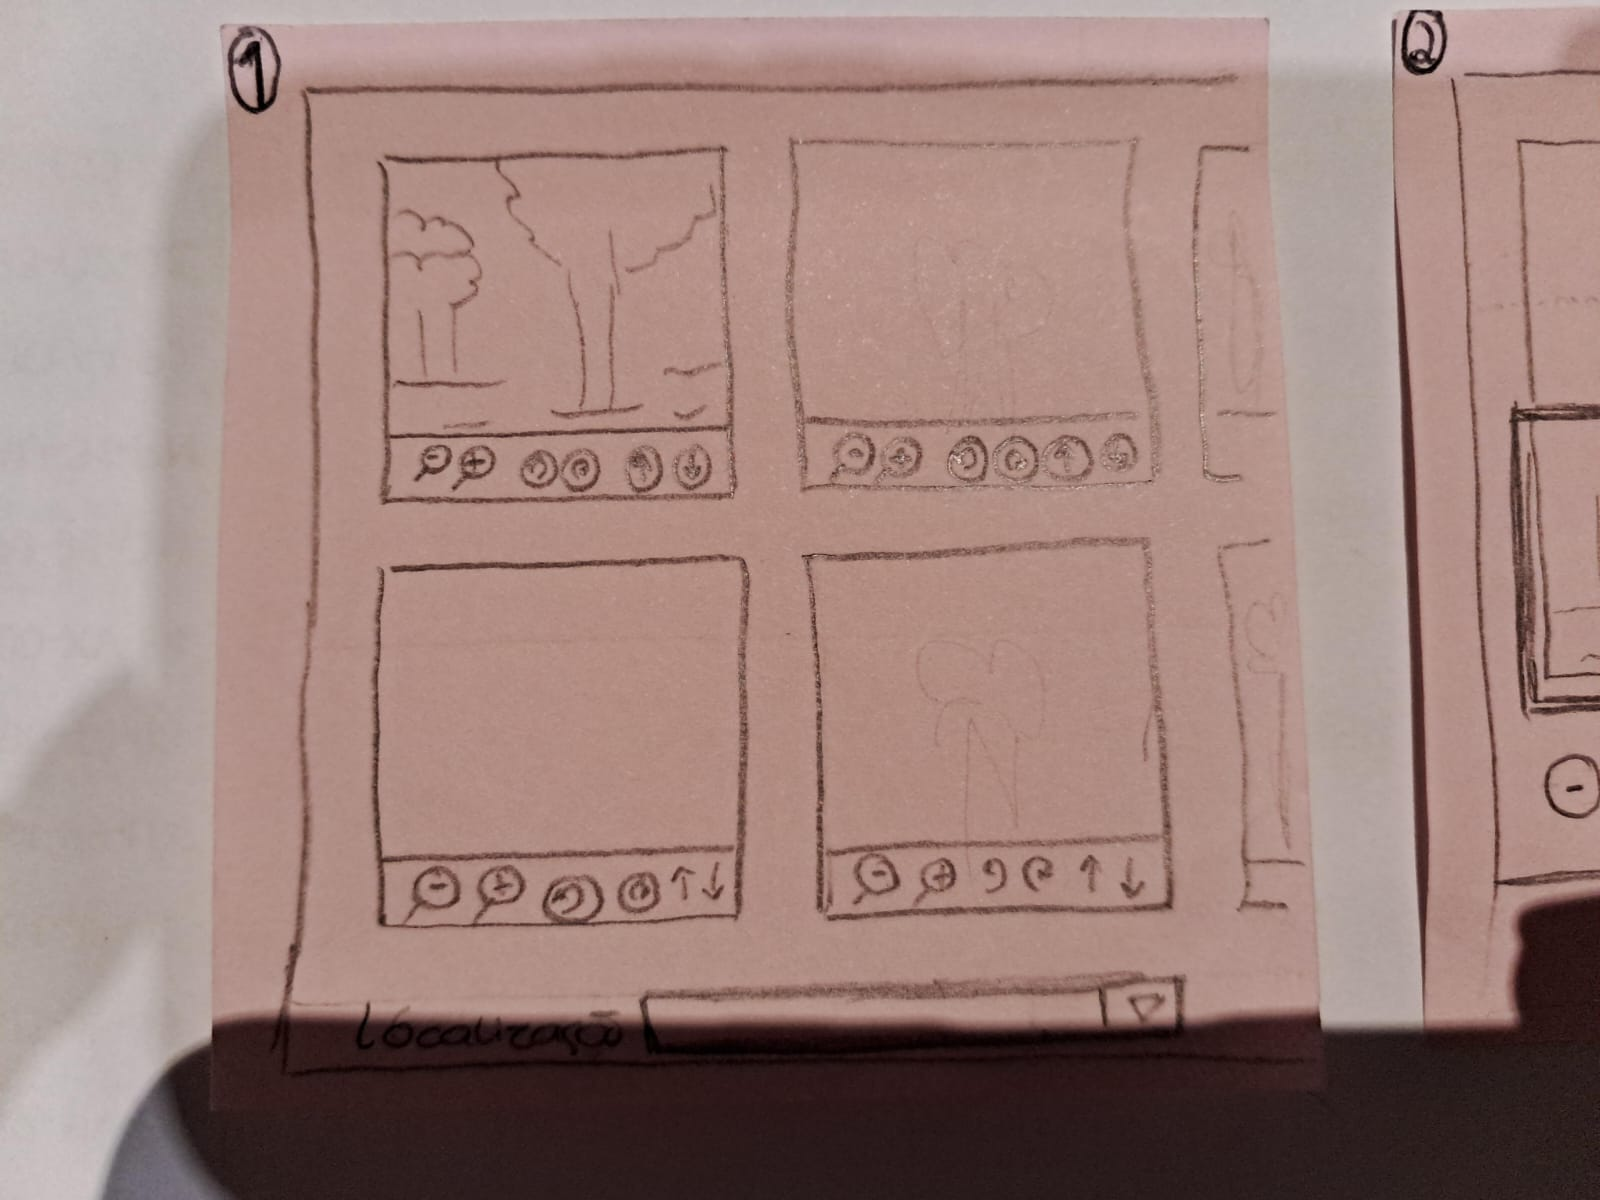
\includegraphics[width=.5\textwidth]{sketches/Cameras_1.jpg}
            }\hfill
            \subfloat[Sketch 2]{
                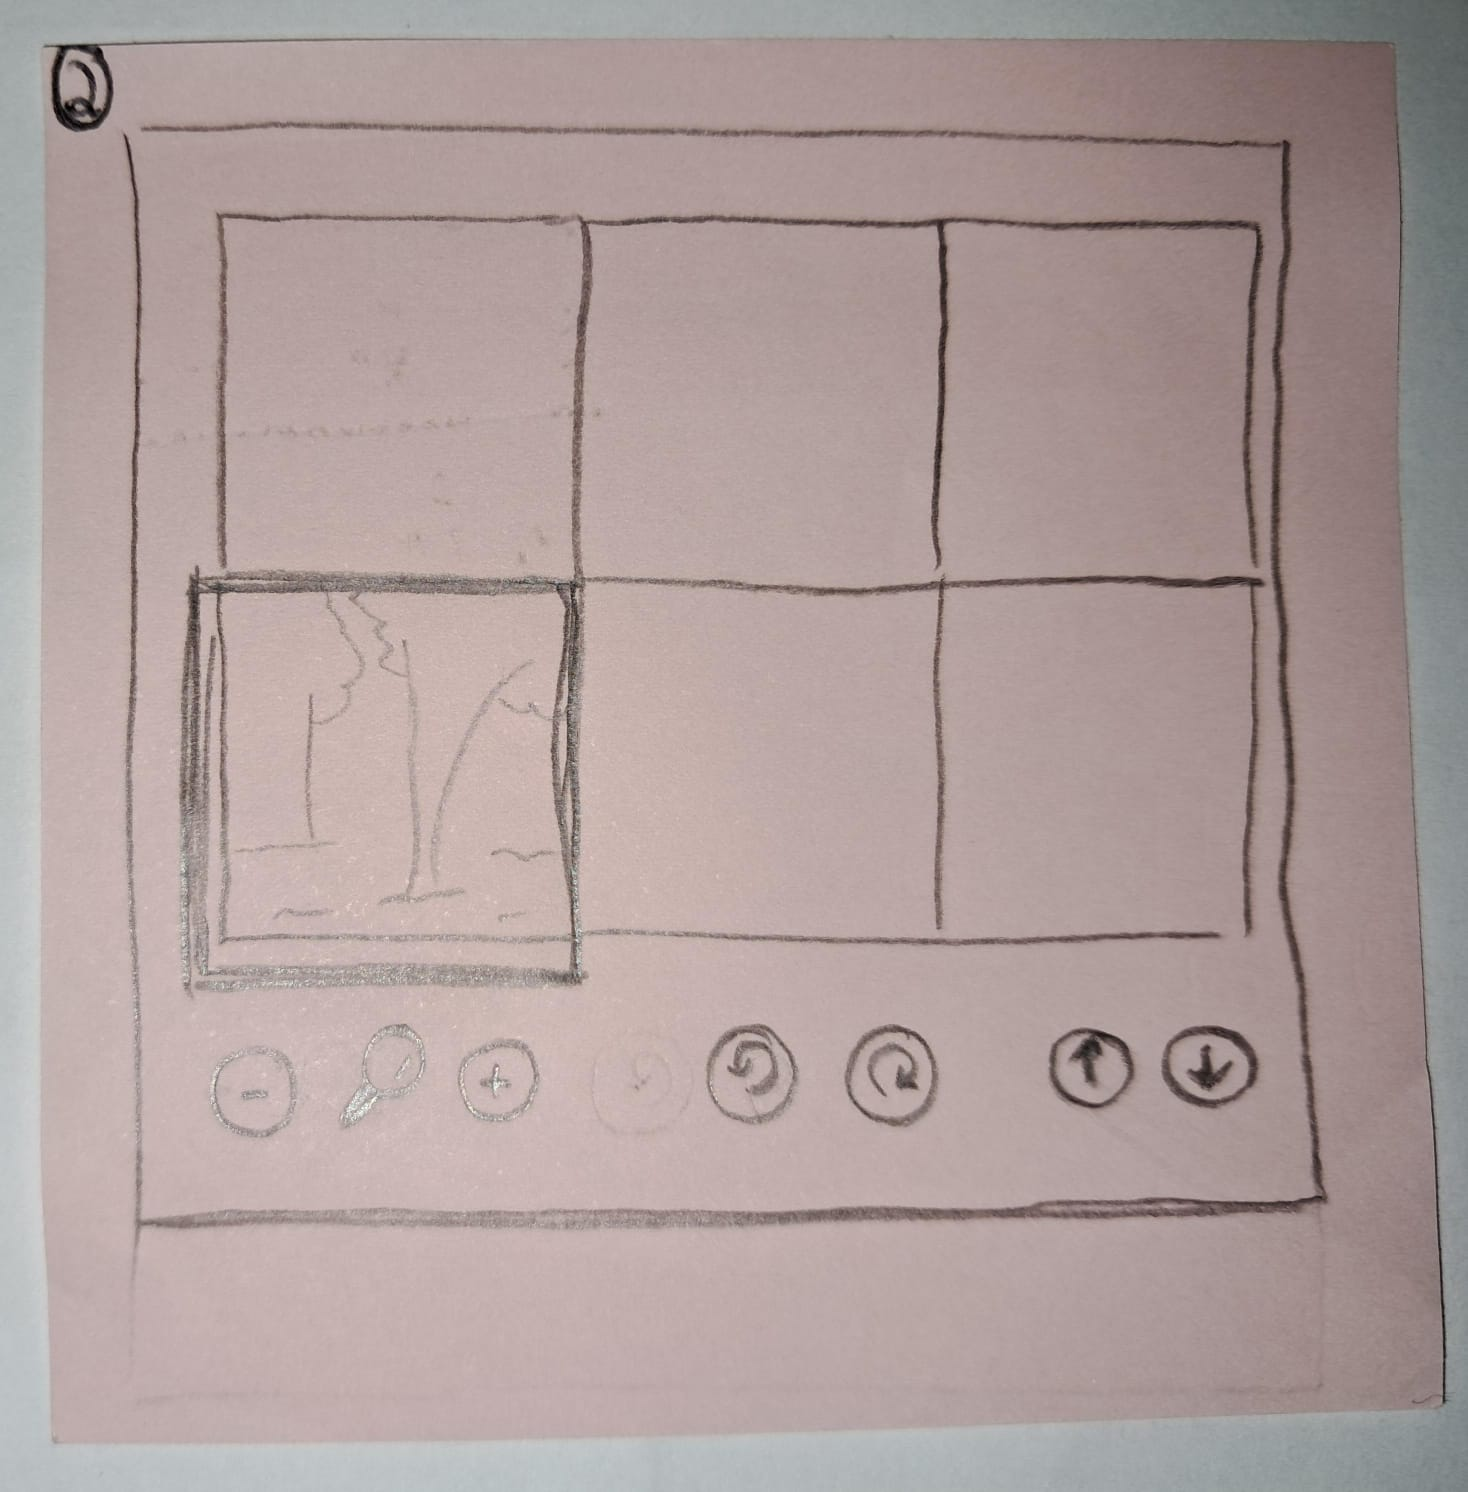
\includegraphics[width=.5\textwidth]{sketches/Cameras_2.jpg}
            }%
            }
        %\end{figure}
        %\begin{figure}[H]\ContinuedFloat
            \centerline{%
            \subfloat[Sketch 3]{
                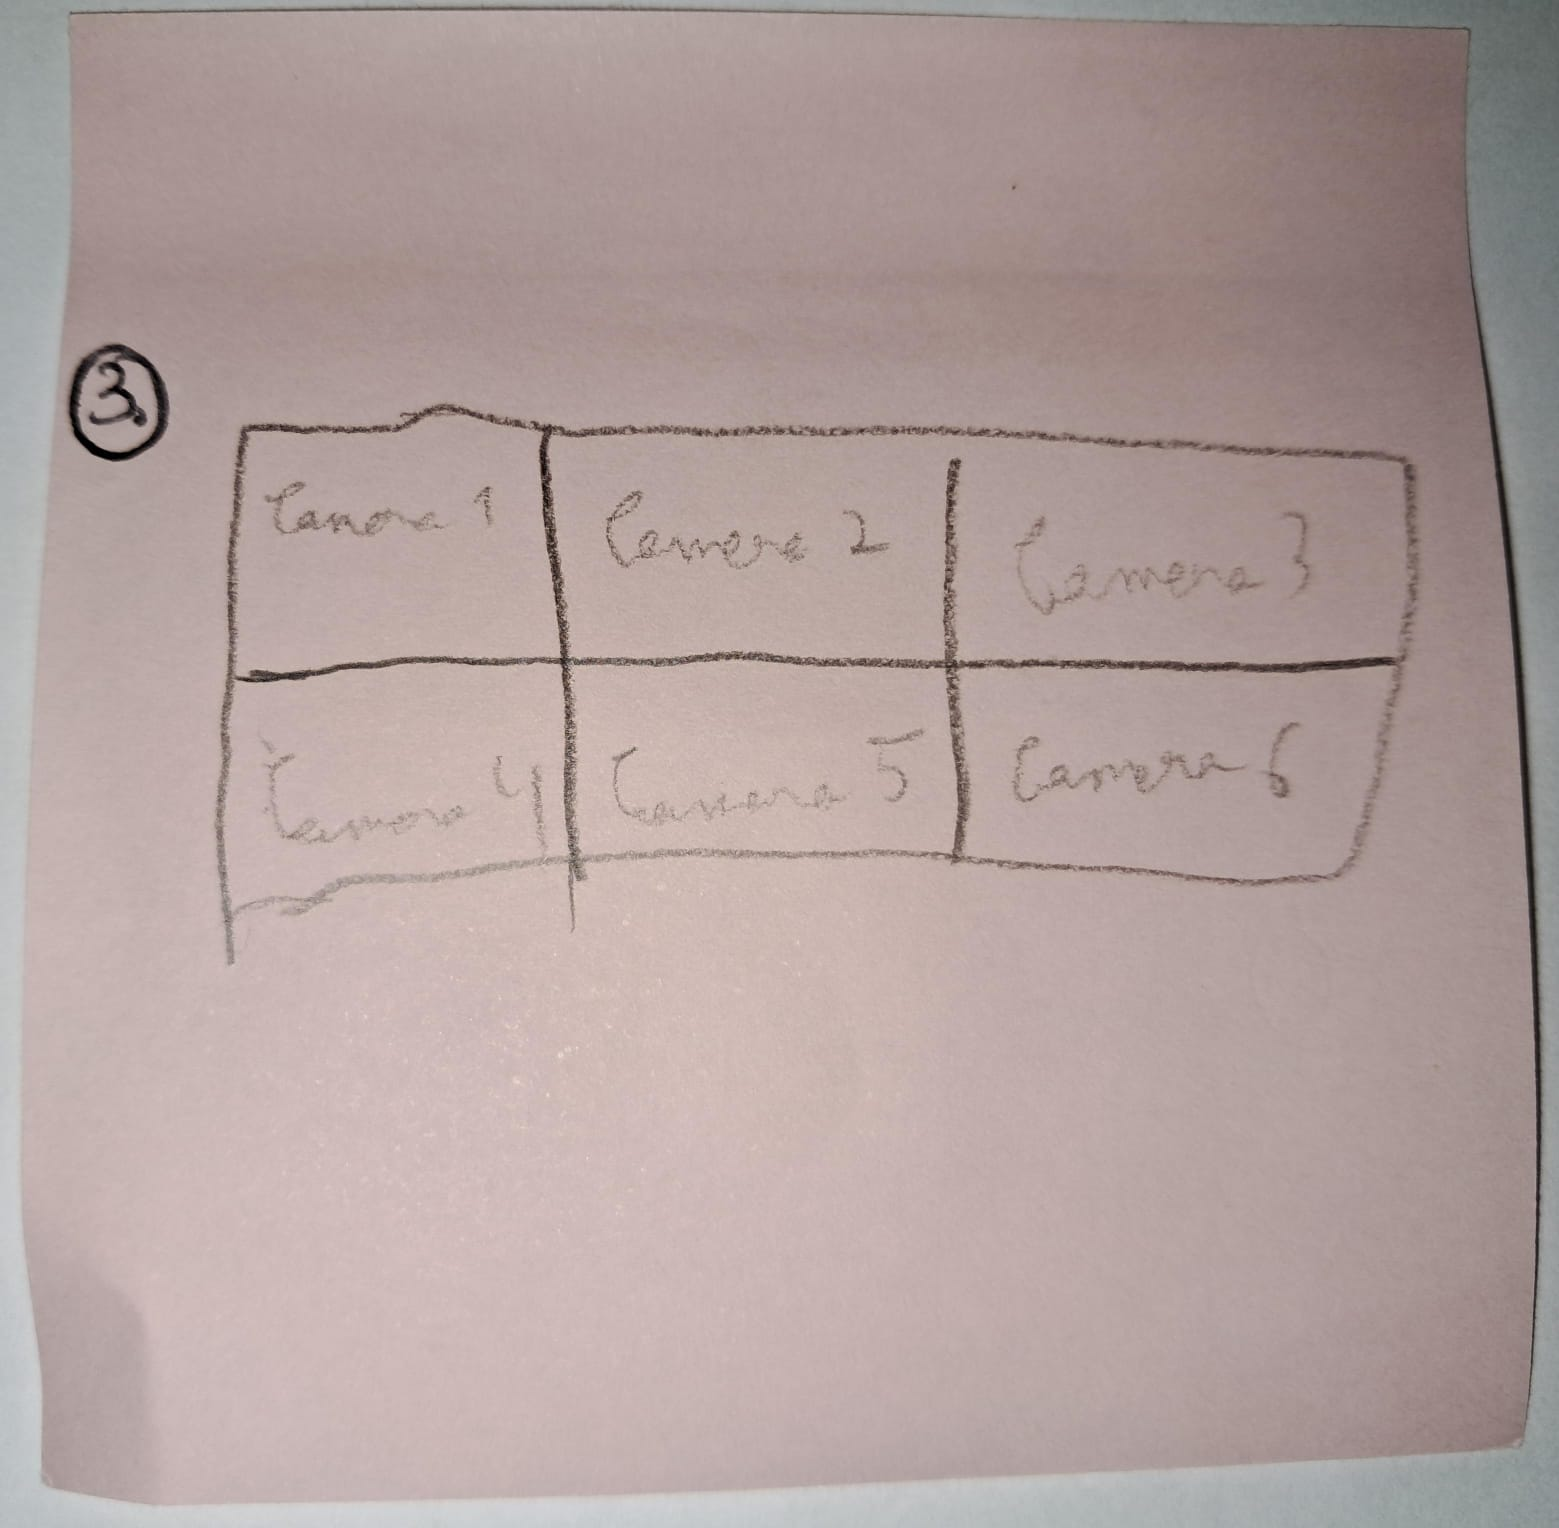
\includegraphics[width=.5\textwidth]{sketches/Cameras_3.jpg}
            }\hfill
            \subfloat[Sketch 4]{
                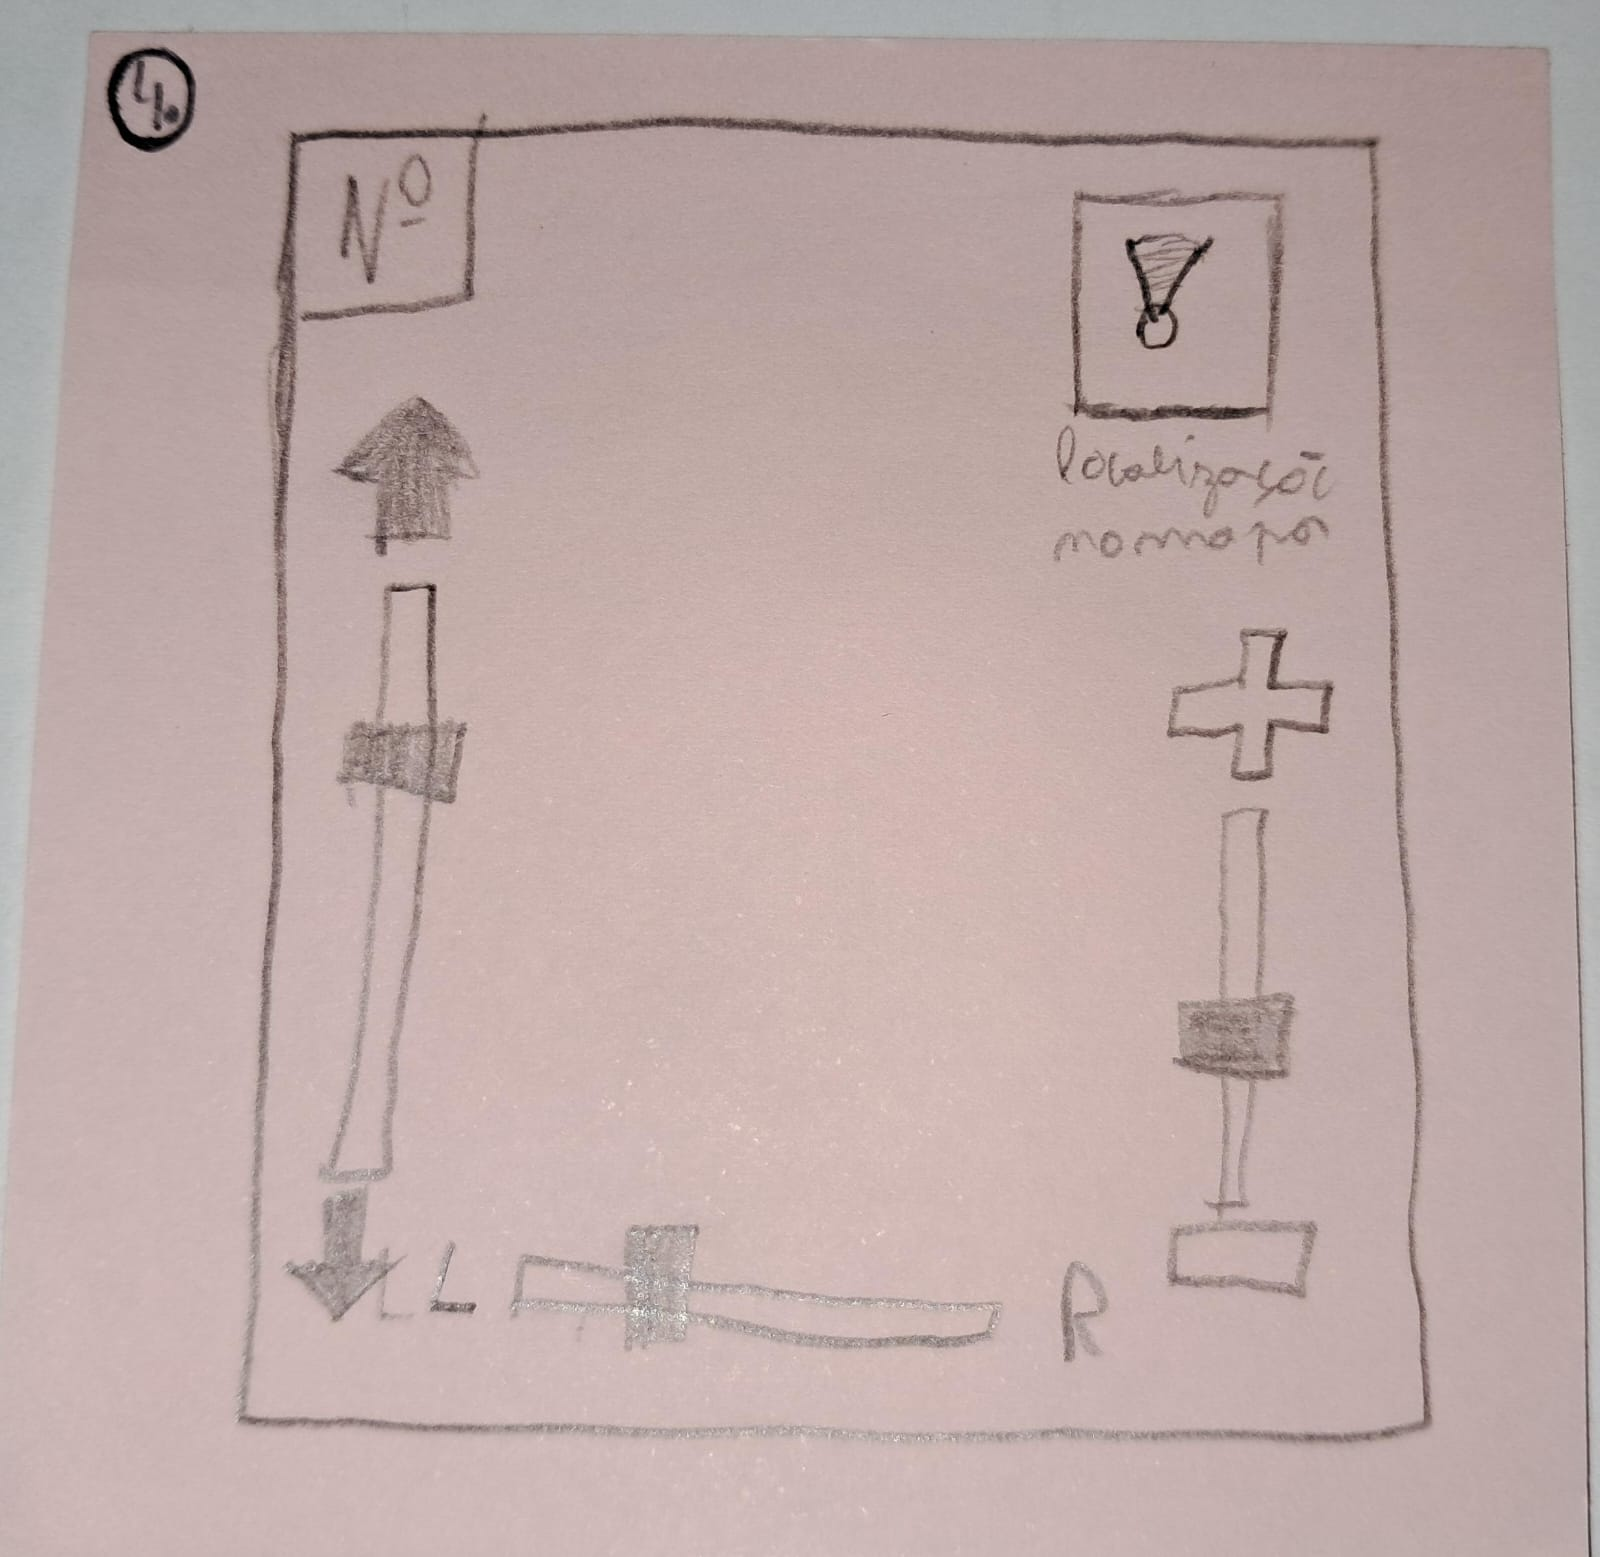
\includegraphics[width=.5\textwidth]{sketches/Cameras_4.jpg}
            }%
            }
            %\end{figure}
            %\begin{figure}[H]\ContinuedFloat
            \centerline{%
            \subfloat[Sketch 5]{
                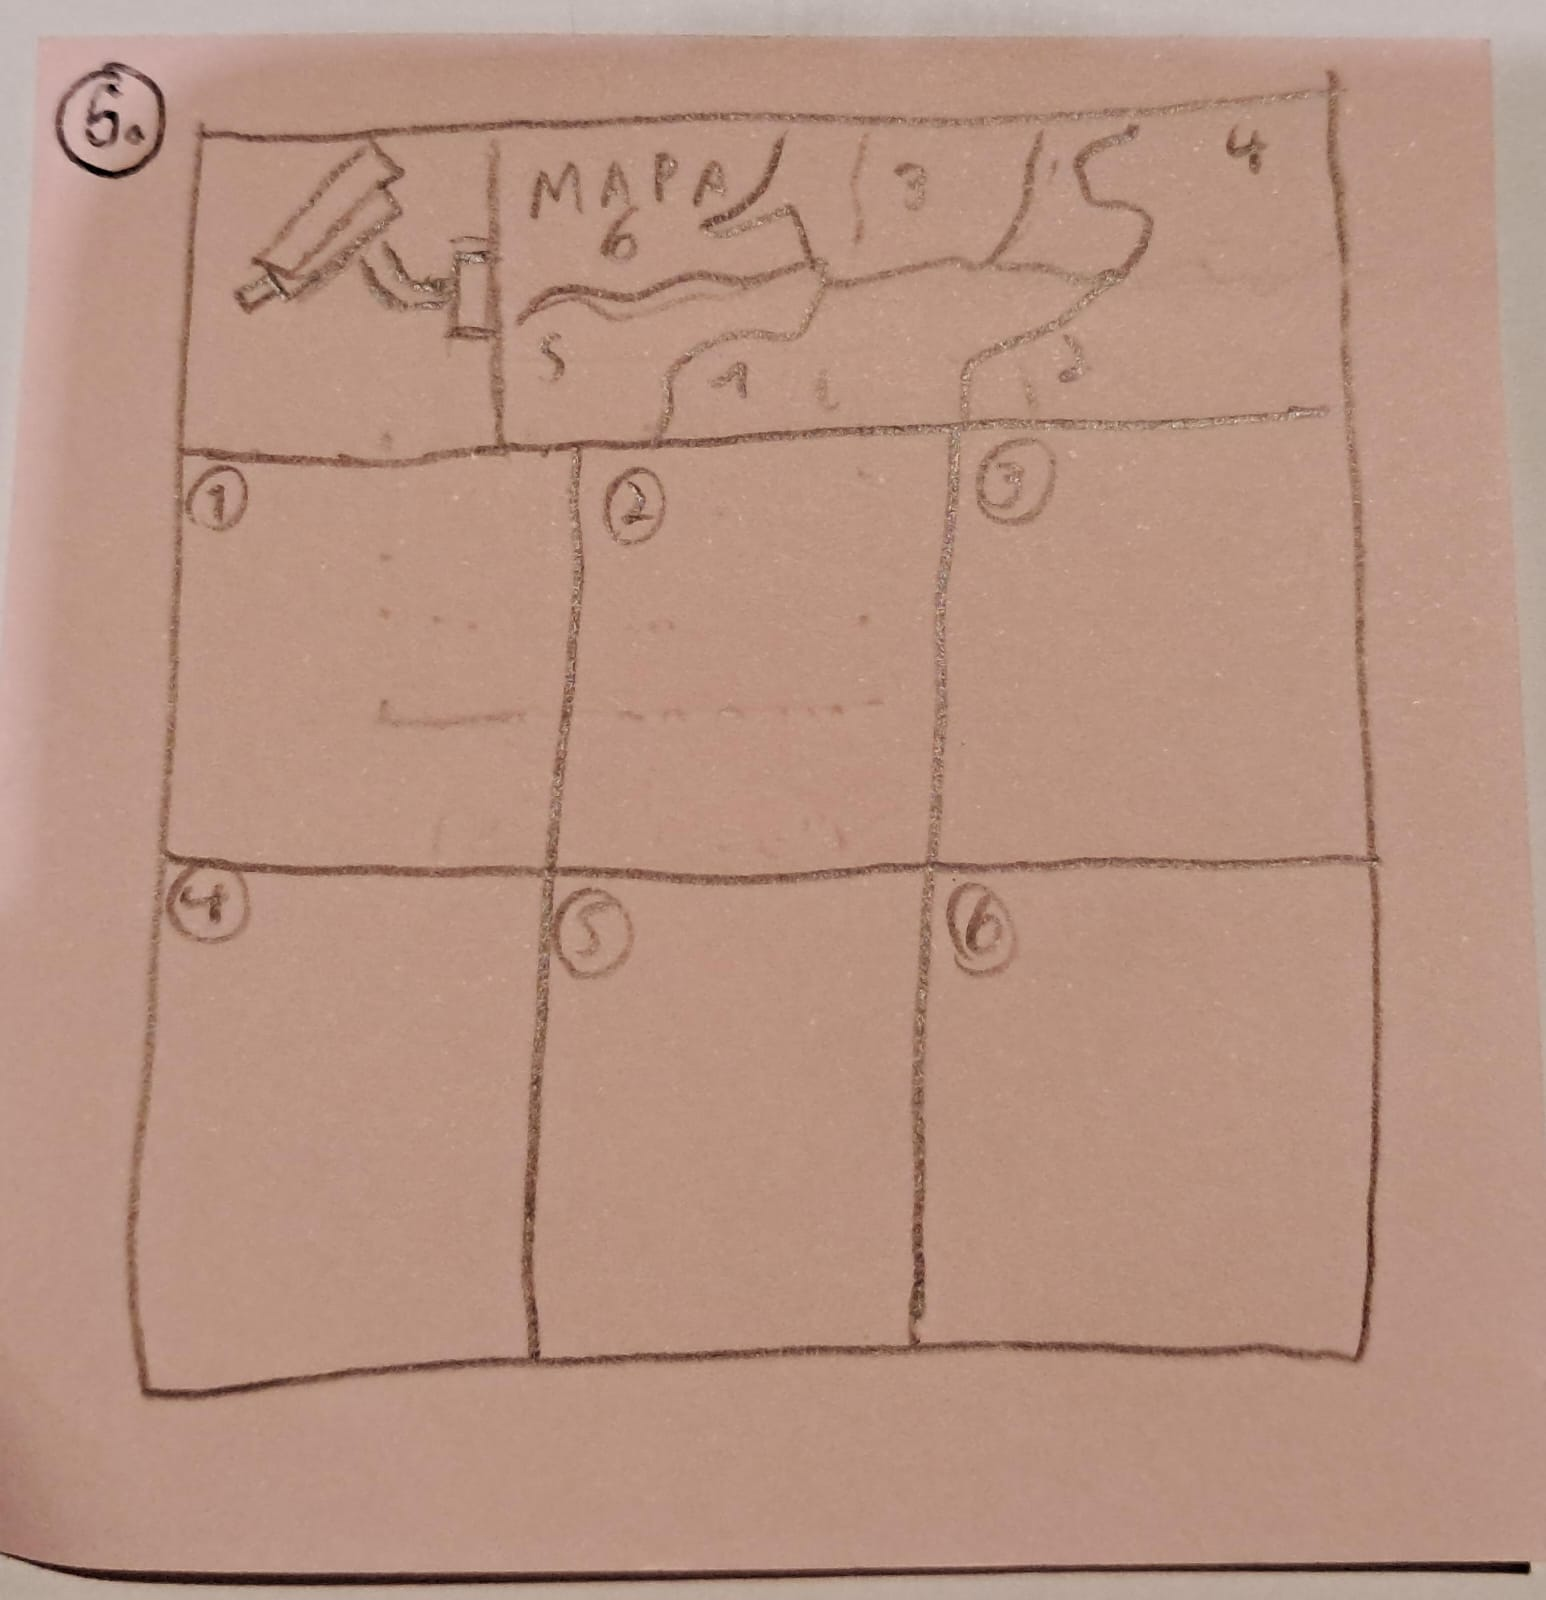
\includegraphics[width=.5\textwidth]{sketches/Cameras_5.jpg}
            }\hfill
            \subfloat[Sketch 6]{
                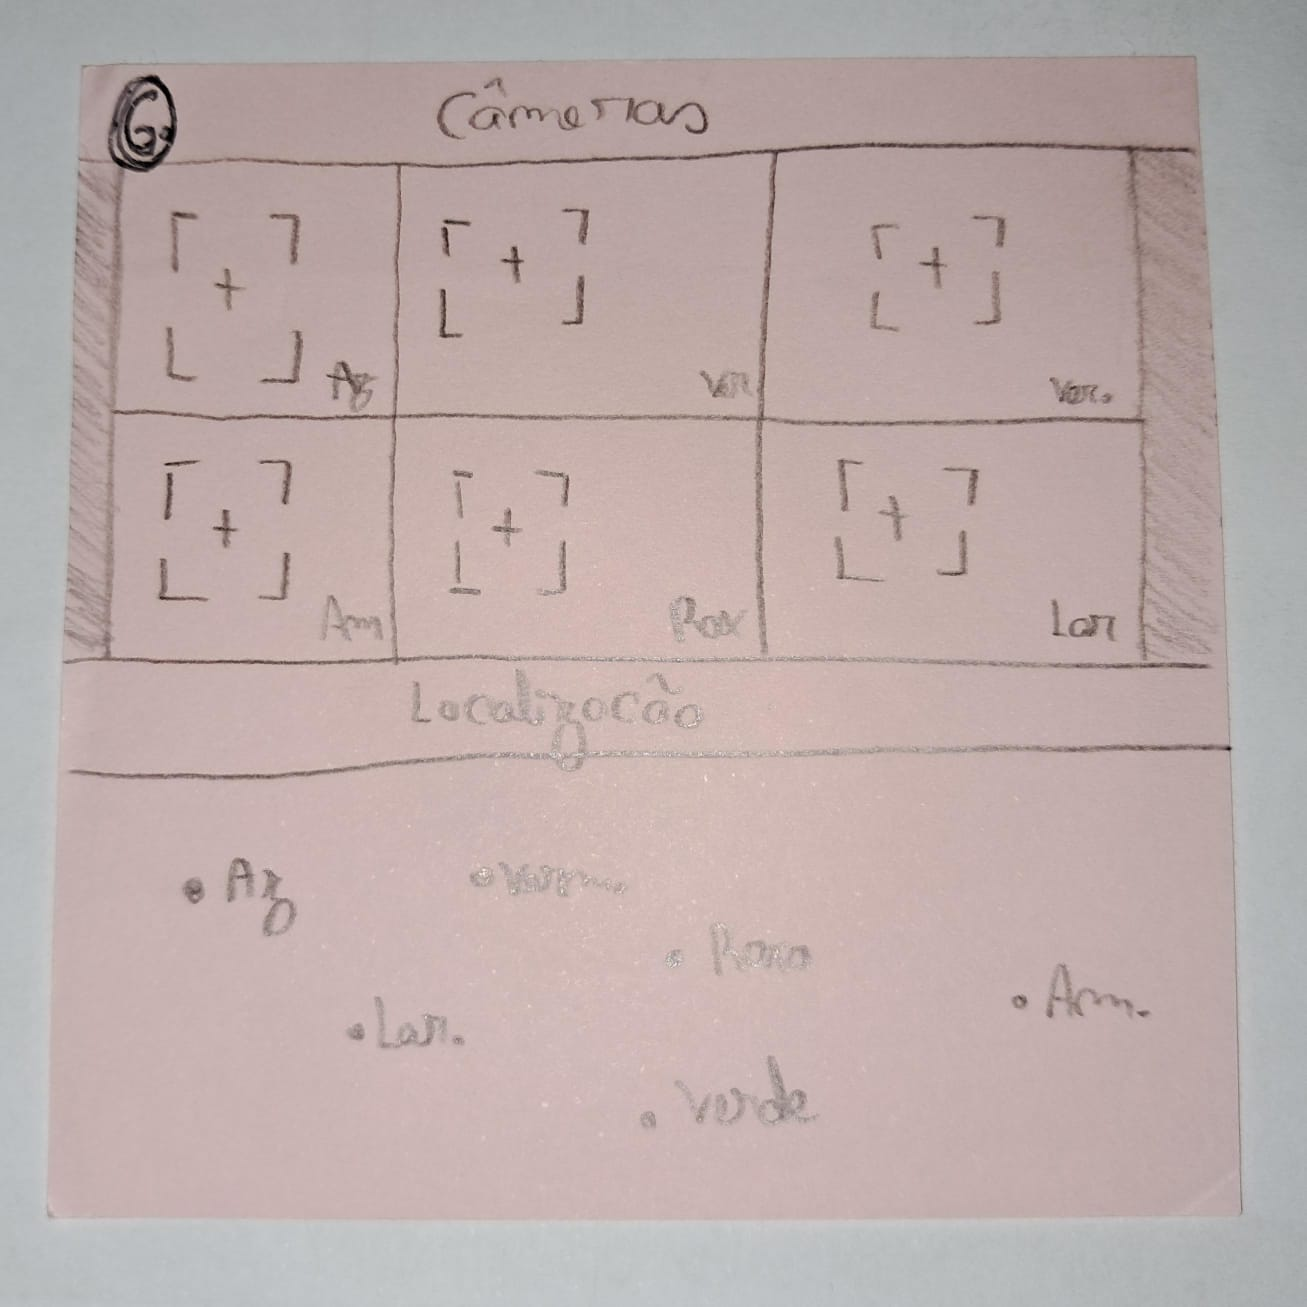
\includegraphics[width=.5\textwidth]{sketches/Cameras_6.jpg}
            }%
            }
            \end{figure}
        \begin{figure}[H]\ContinuedFloat
            \centerline{%
            \subfloat[Sketch 7]{
                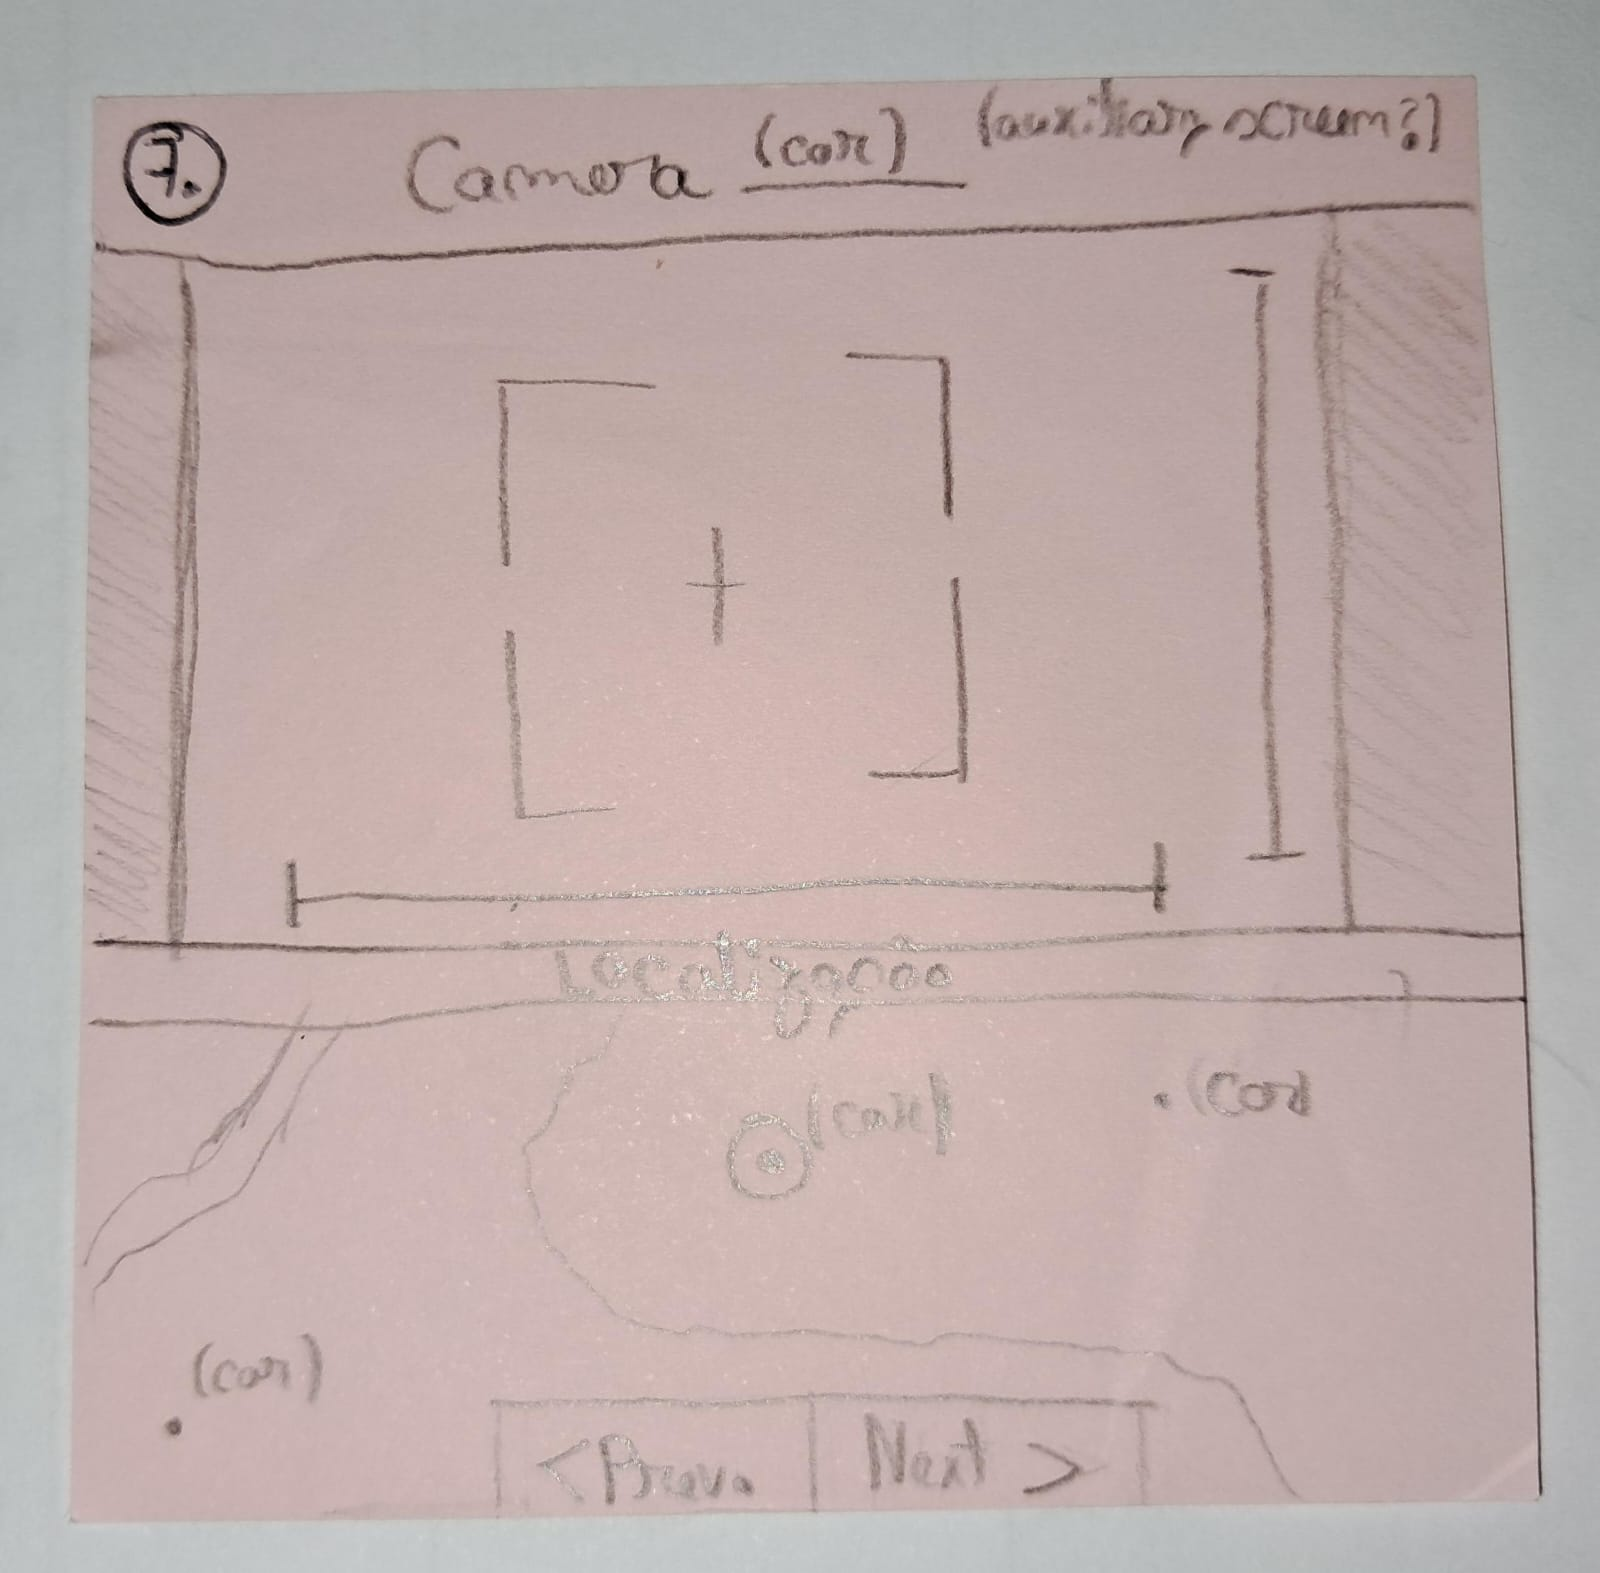
\includegraphics[width=.4\textwidth]{sketches/Cameras_7.jpg}
            }\hfill
            \subfloat[Sketch 8]{
                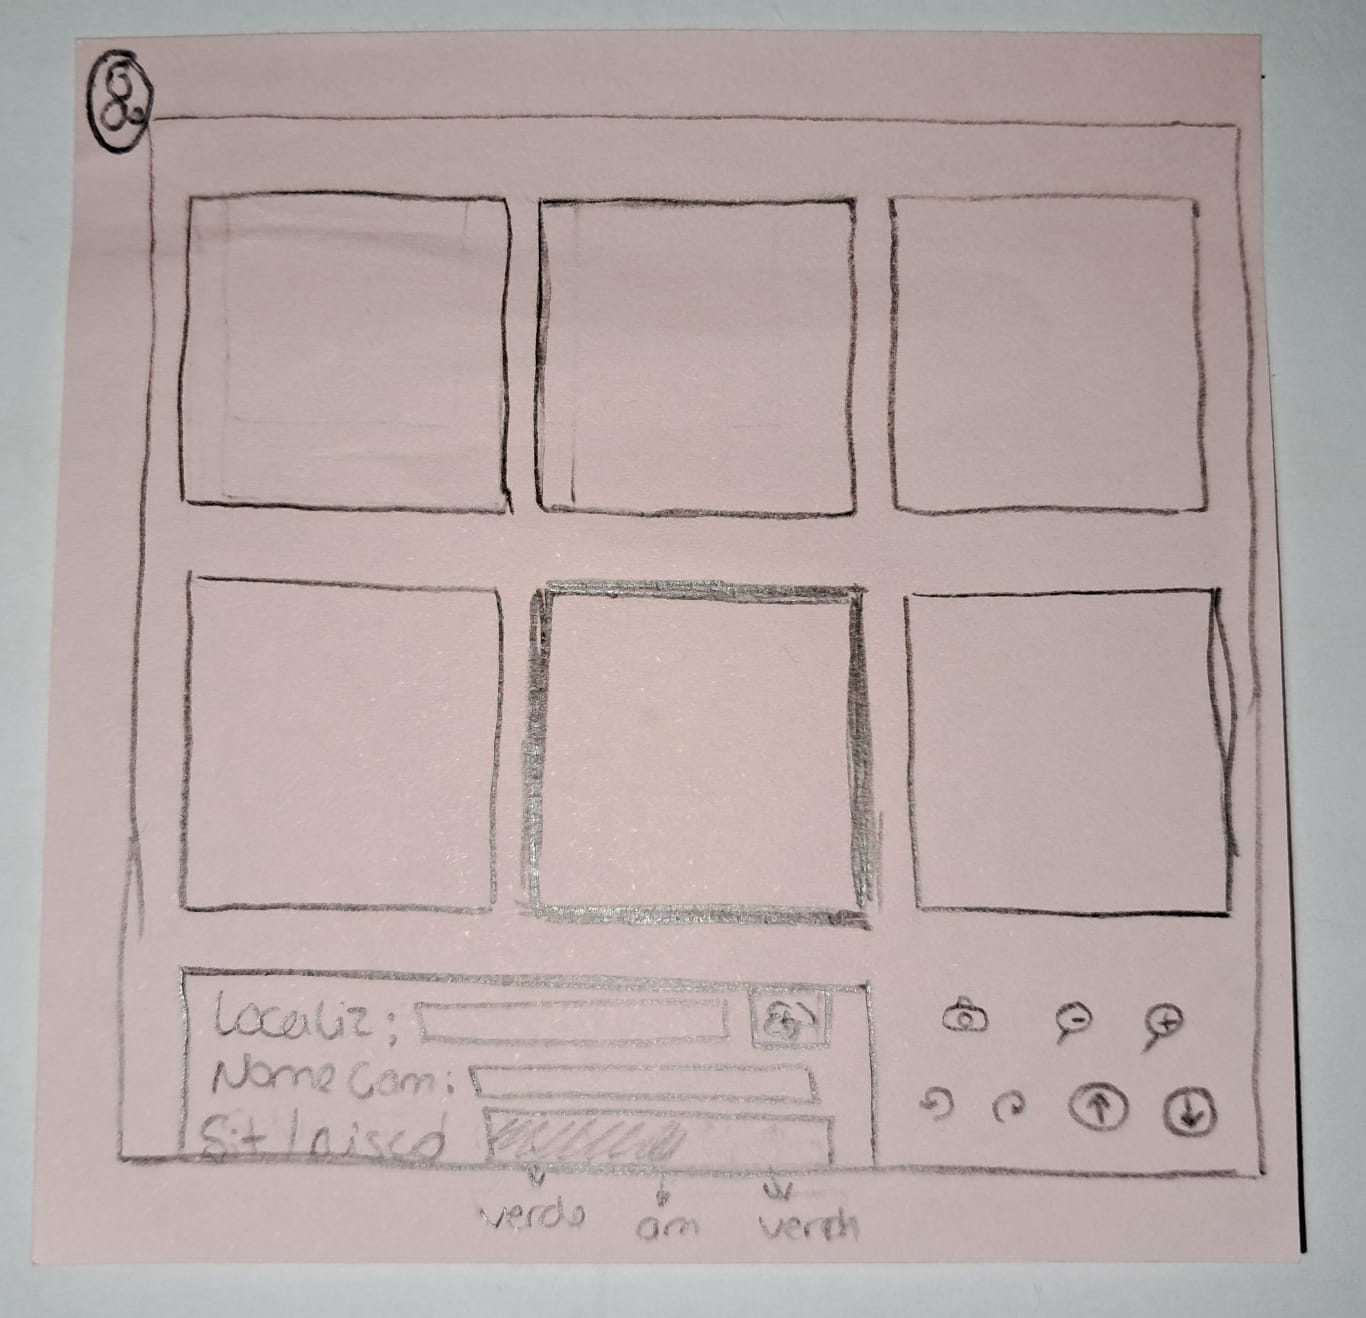
\includegraphics[width=.4\textwidth]{sketches/Cameras_8.jpg}
            }\hfill
            \subfloat[Sketch 9]{
                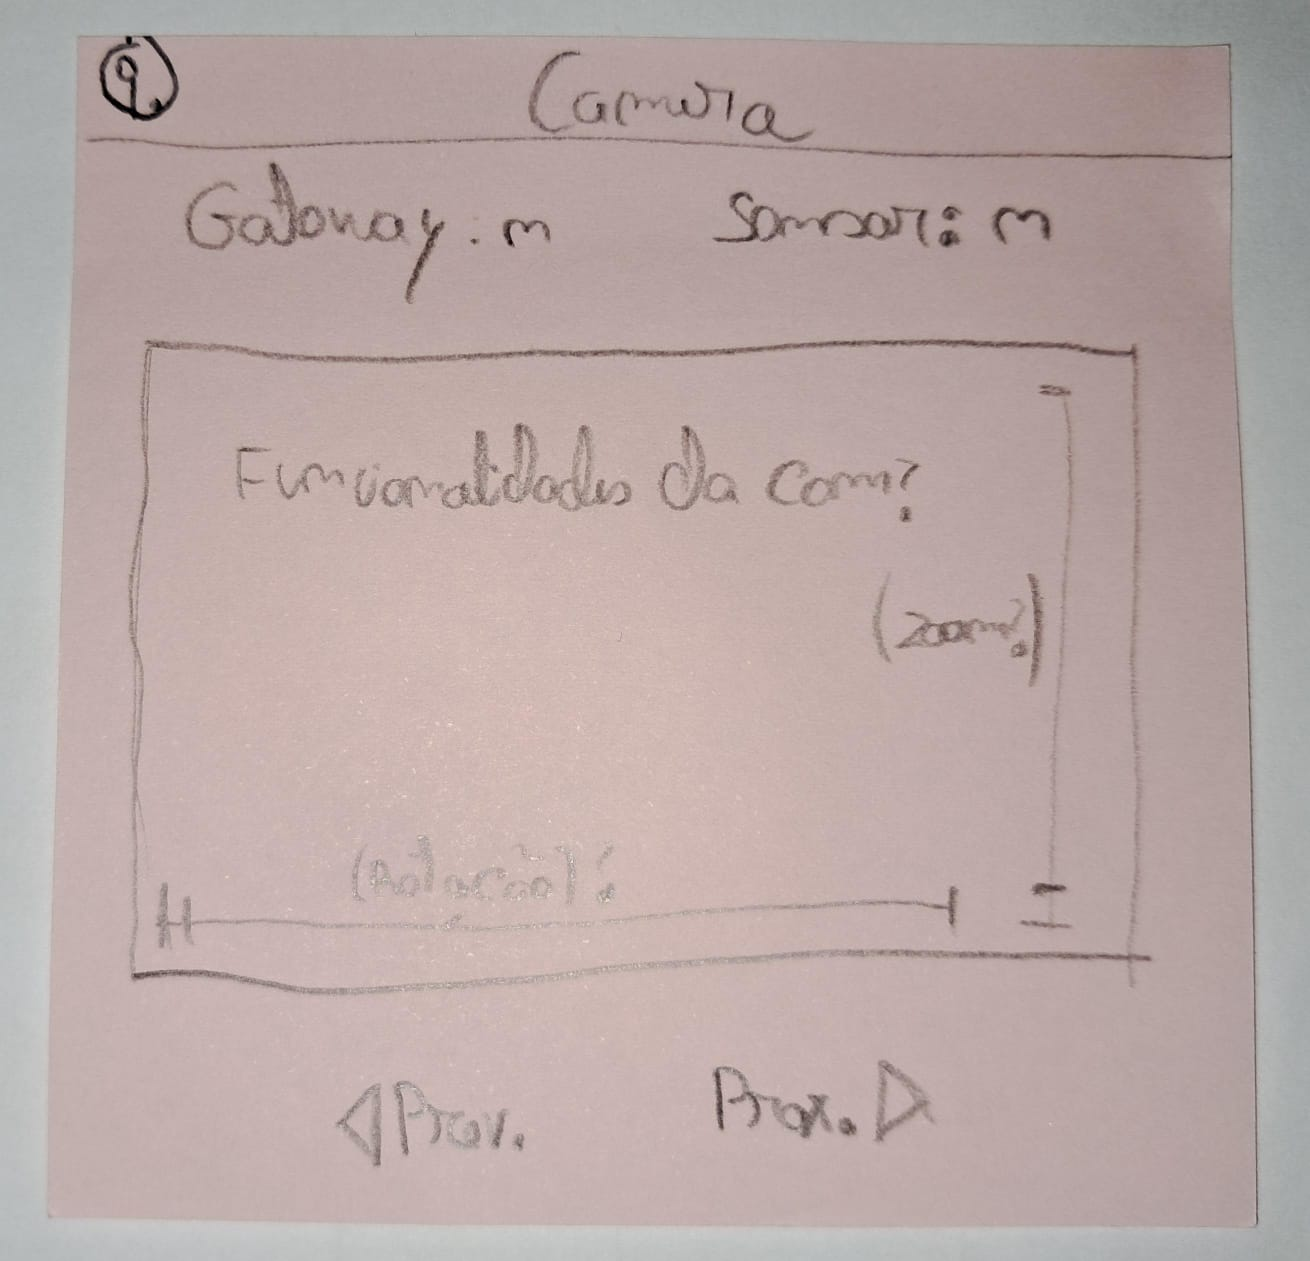
\includegraphics[width=.4\textwidth]{sketches/Cameras_9.jpg}
            }%
            }
            \caption{Camera Panel Sketches}
        \end{figure}
    \item \textbf{Log Panel:}
        \begin{figure}[H]
            \centerline{%
            \subfloat[Sketch 1]{
                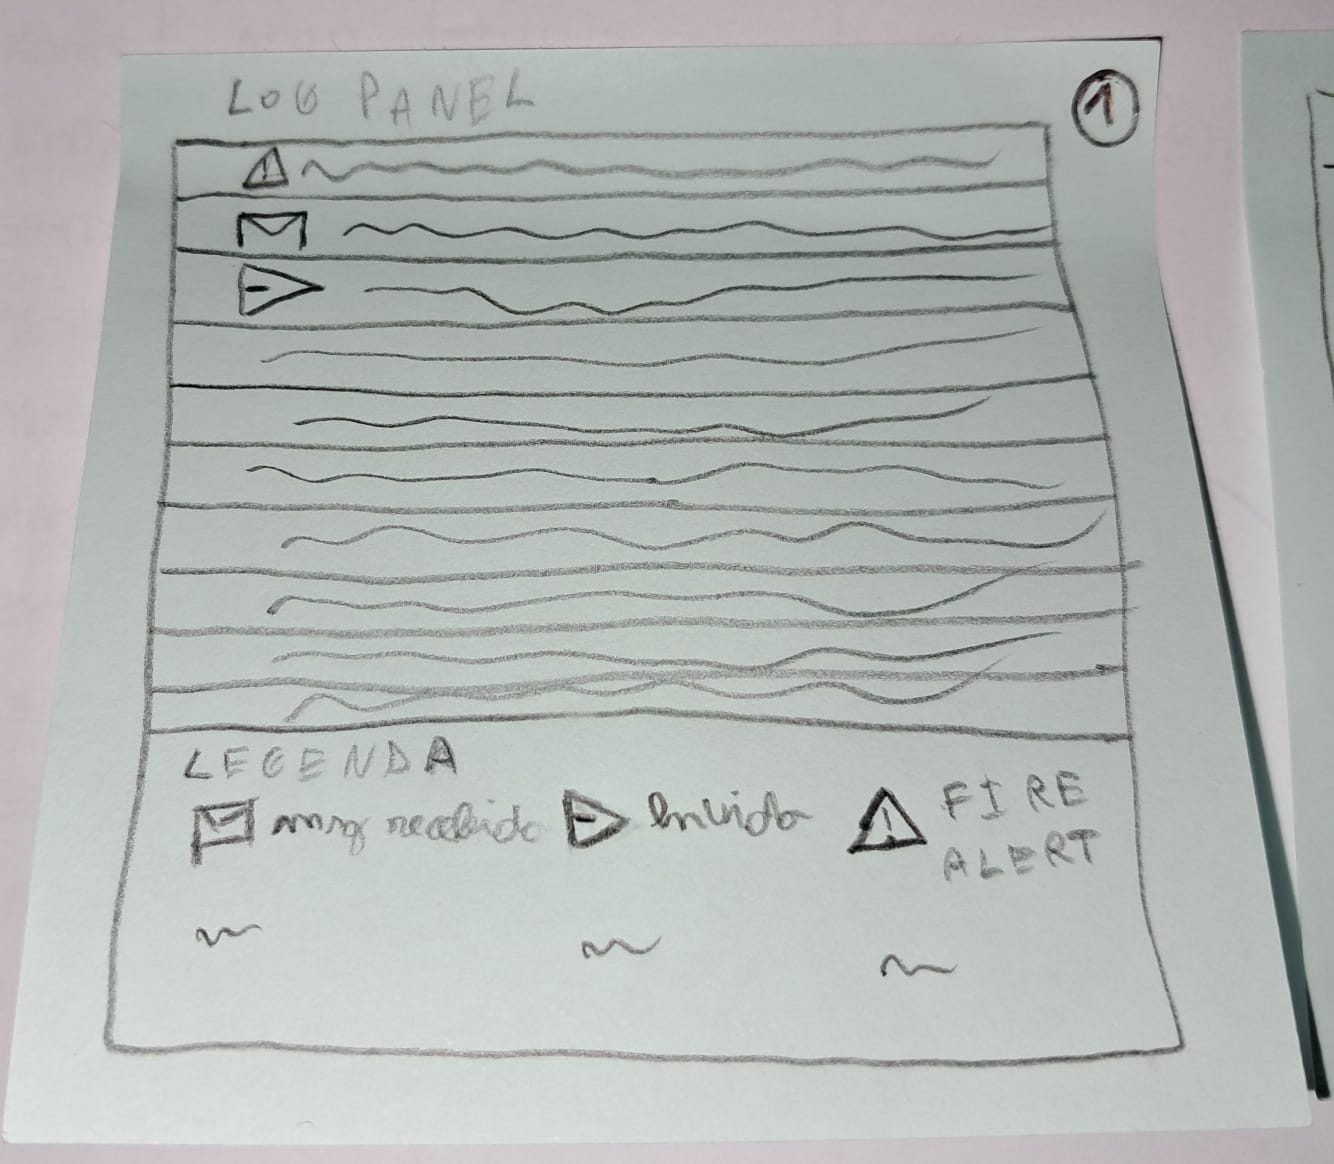
\includegraphics[width=.5\textwidth]{sketches/Log_1.jpg}
            }\hfill
            \subfloat[Sketch 2]{
                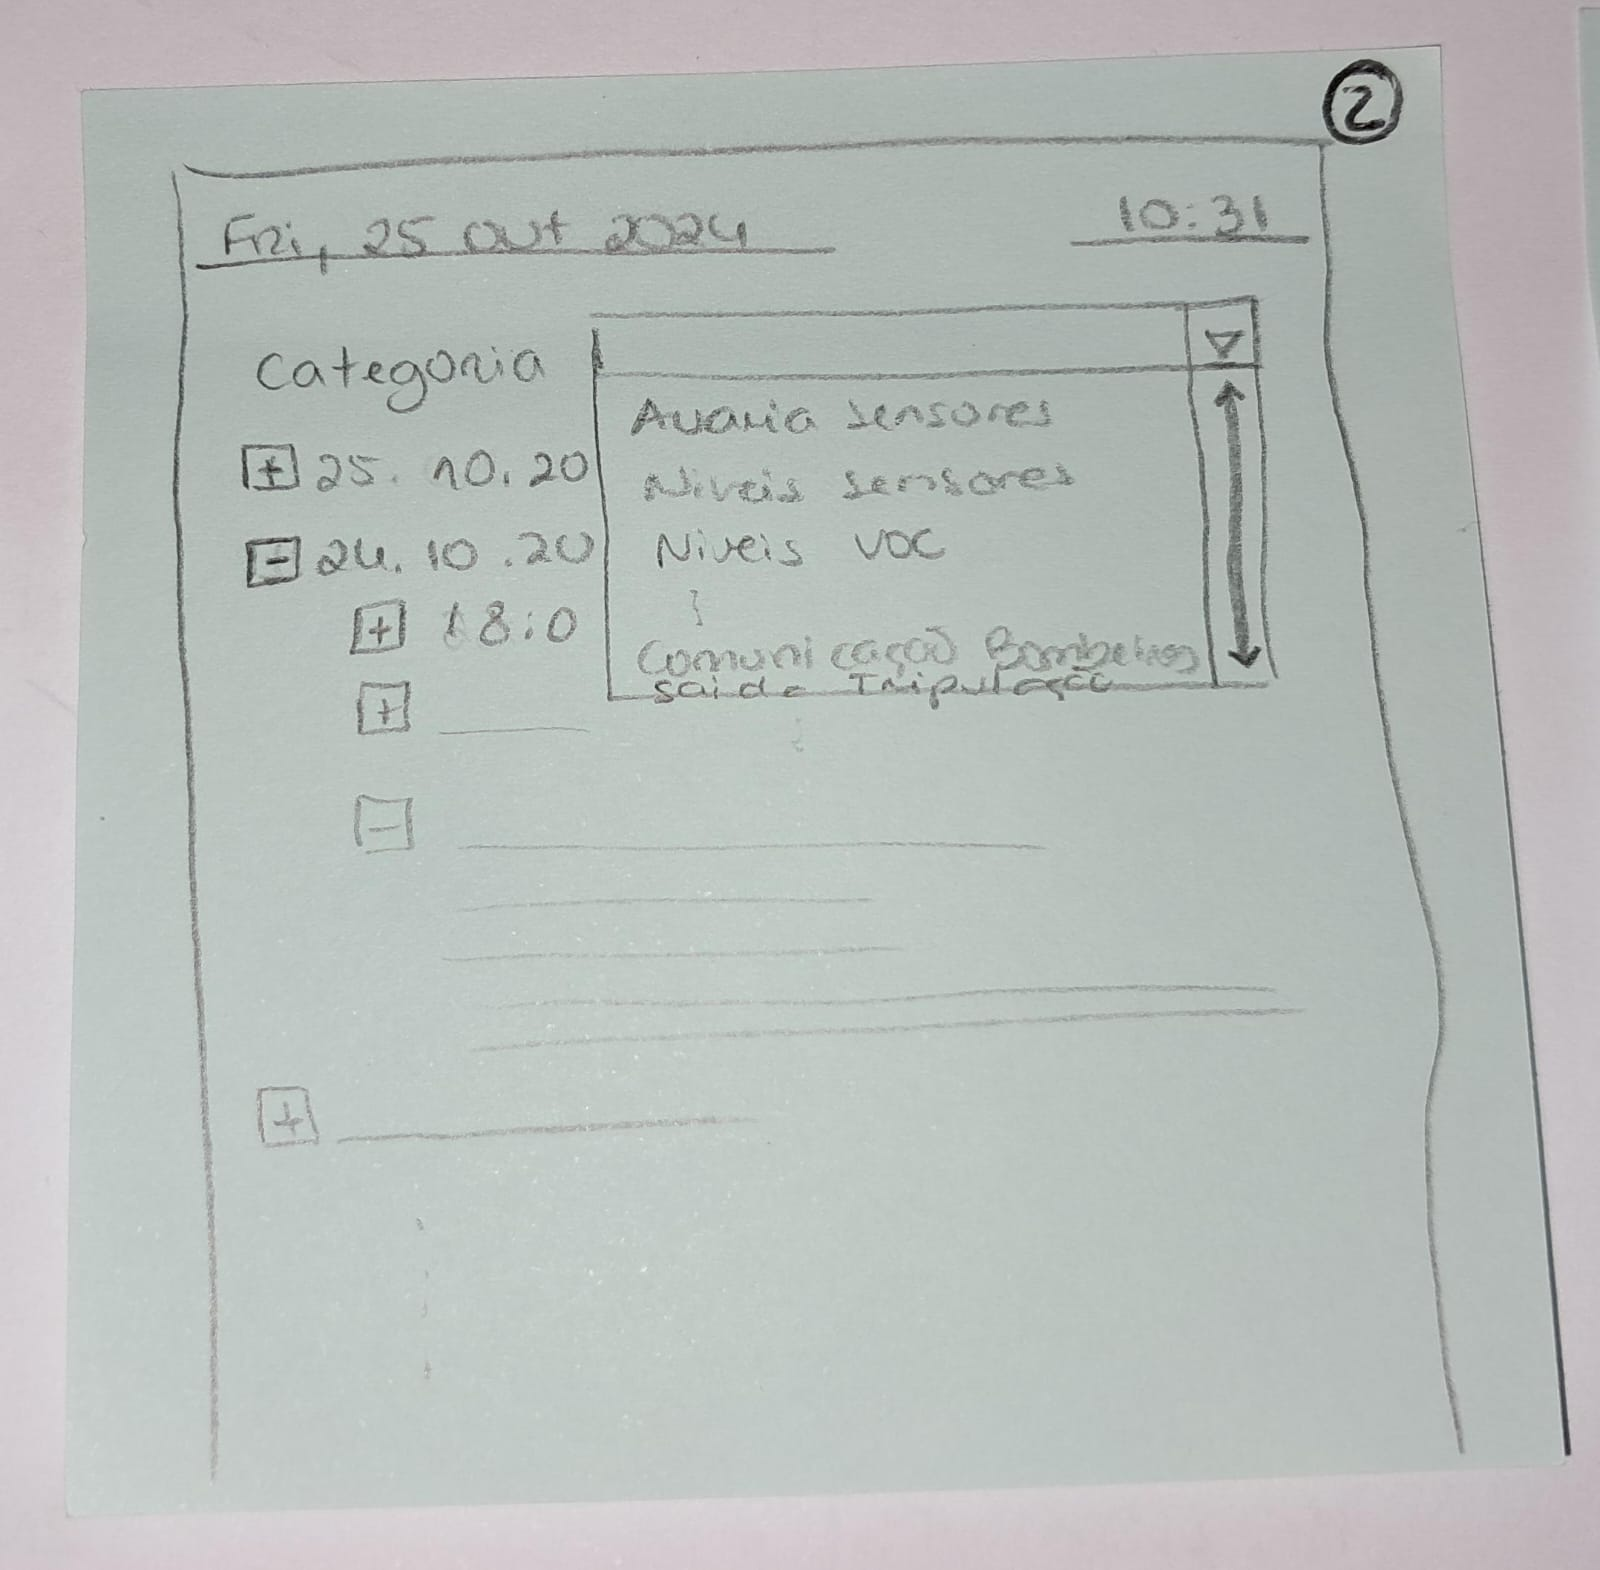
\includegraphics[width=.5\textwidth]{sketches/Log_2.jpg}
            }%
            }
        \end{figure}
        \begin{figure}[H]\ContinuedFloat
            \centerline{%
            \subfloat[Sketch 3]{
                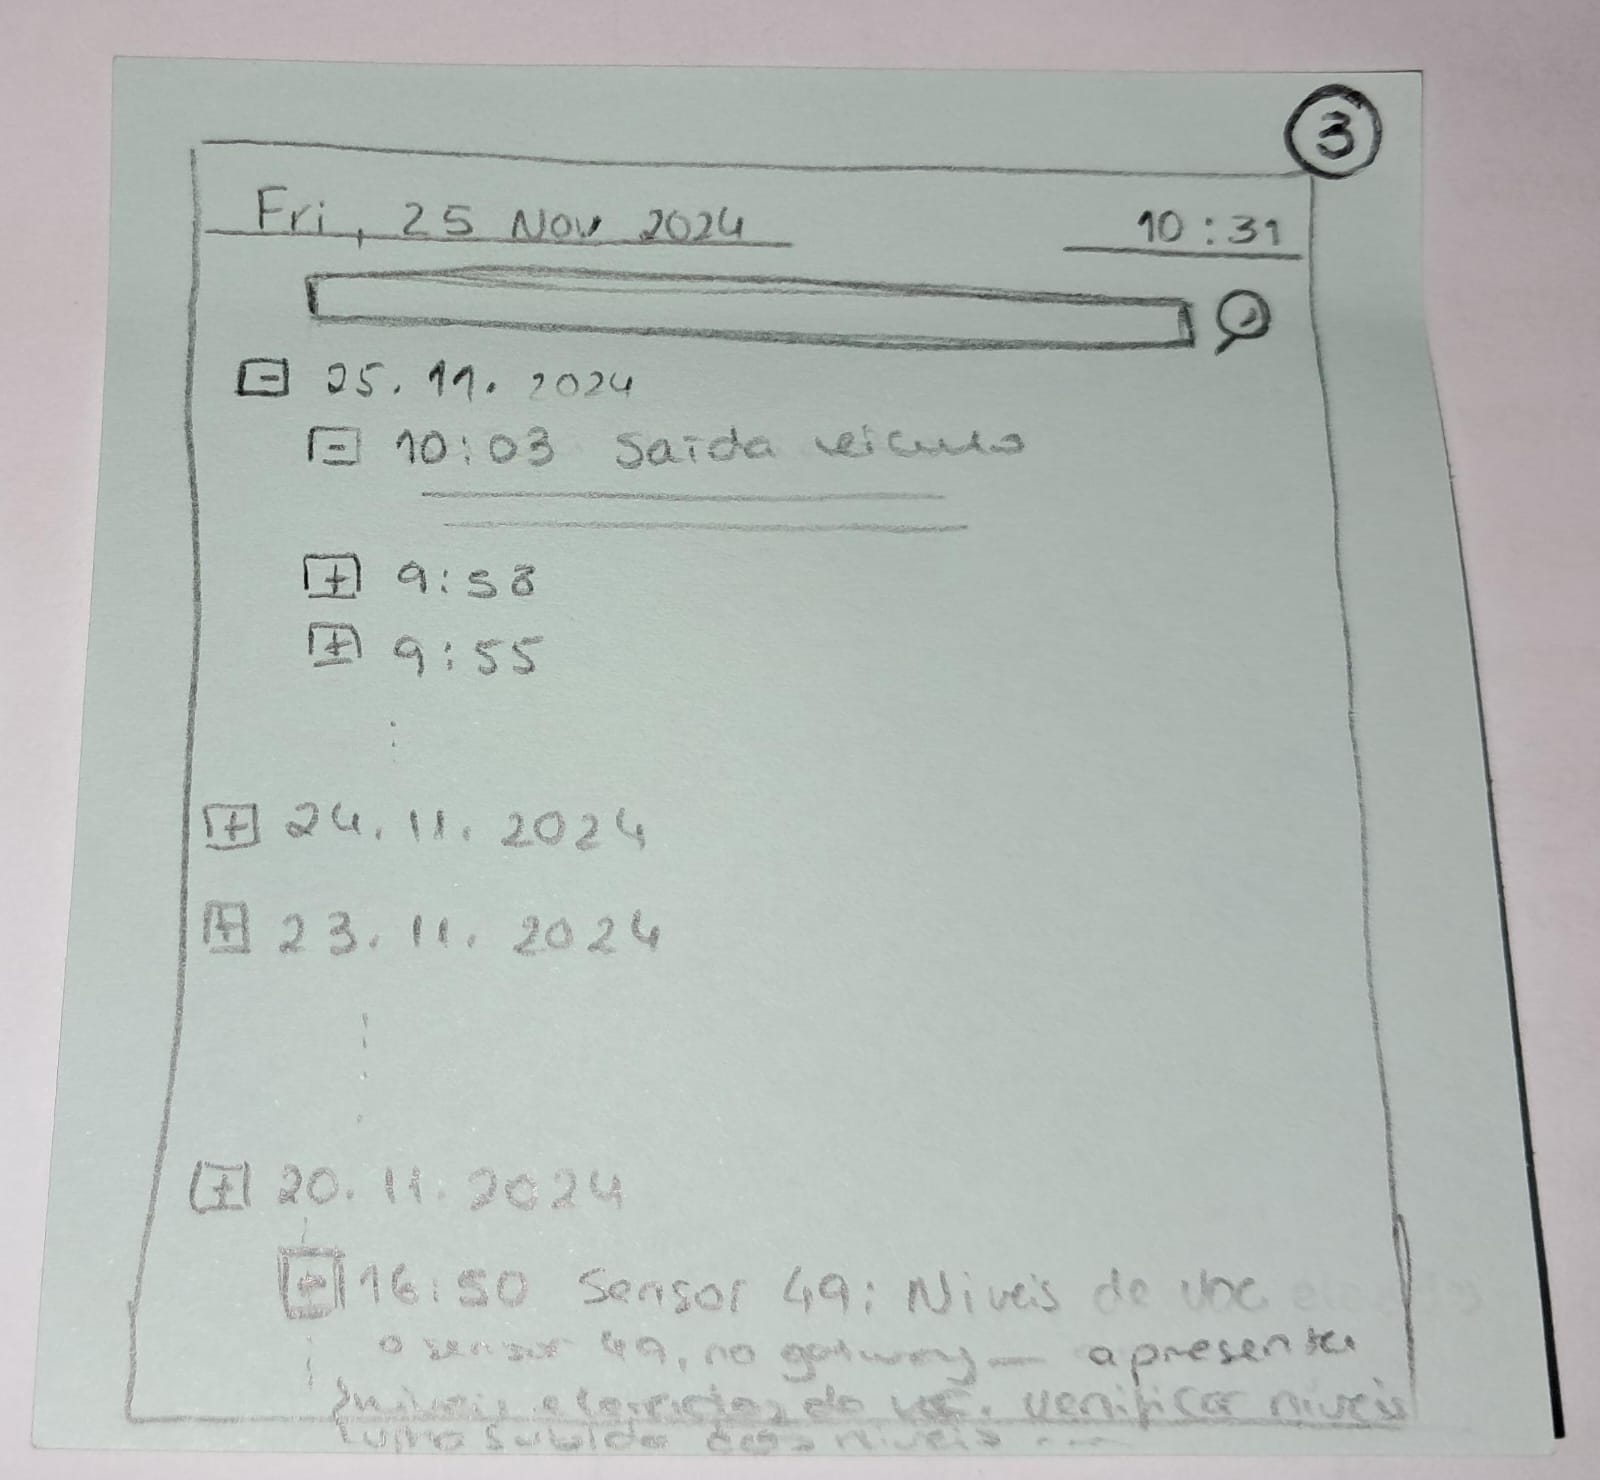
\includegraphics[width=.5\textwidth]{sketches/Log_3.jpg}
            }\hfill
            \subfloat[Sketch 4]{
                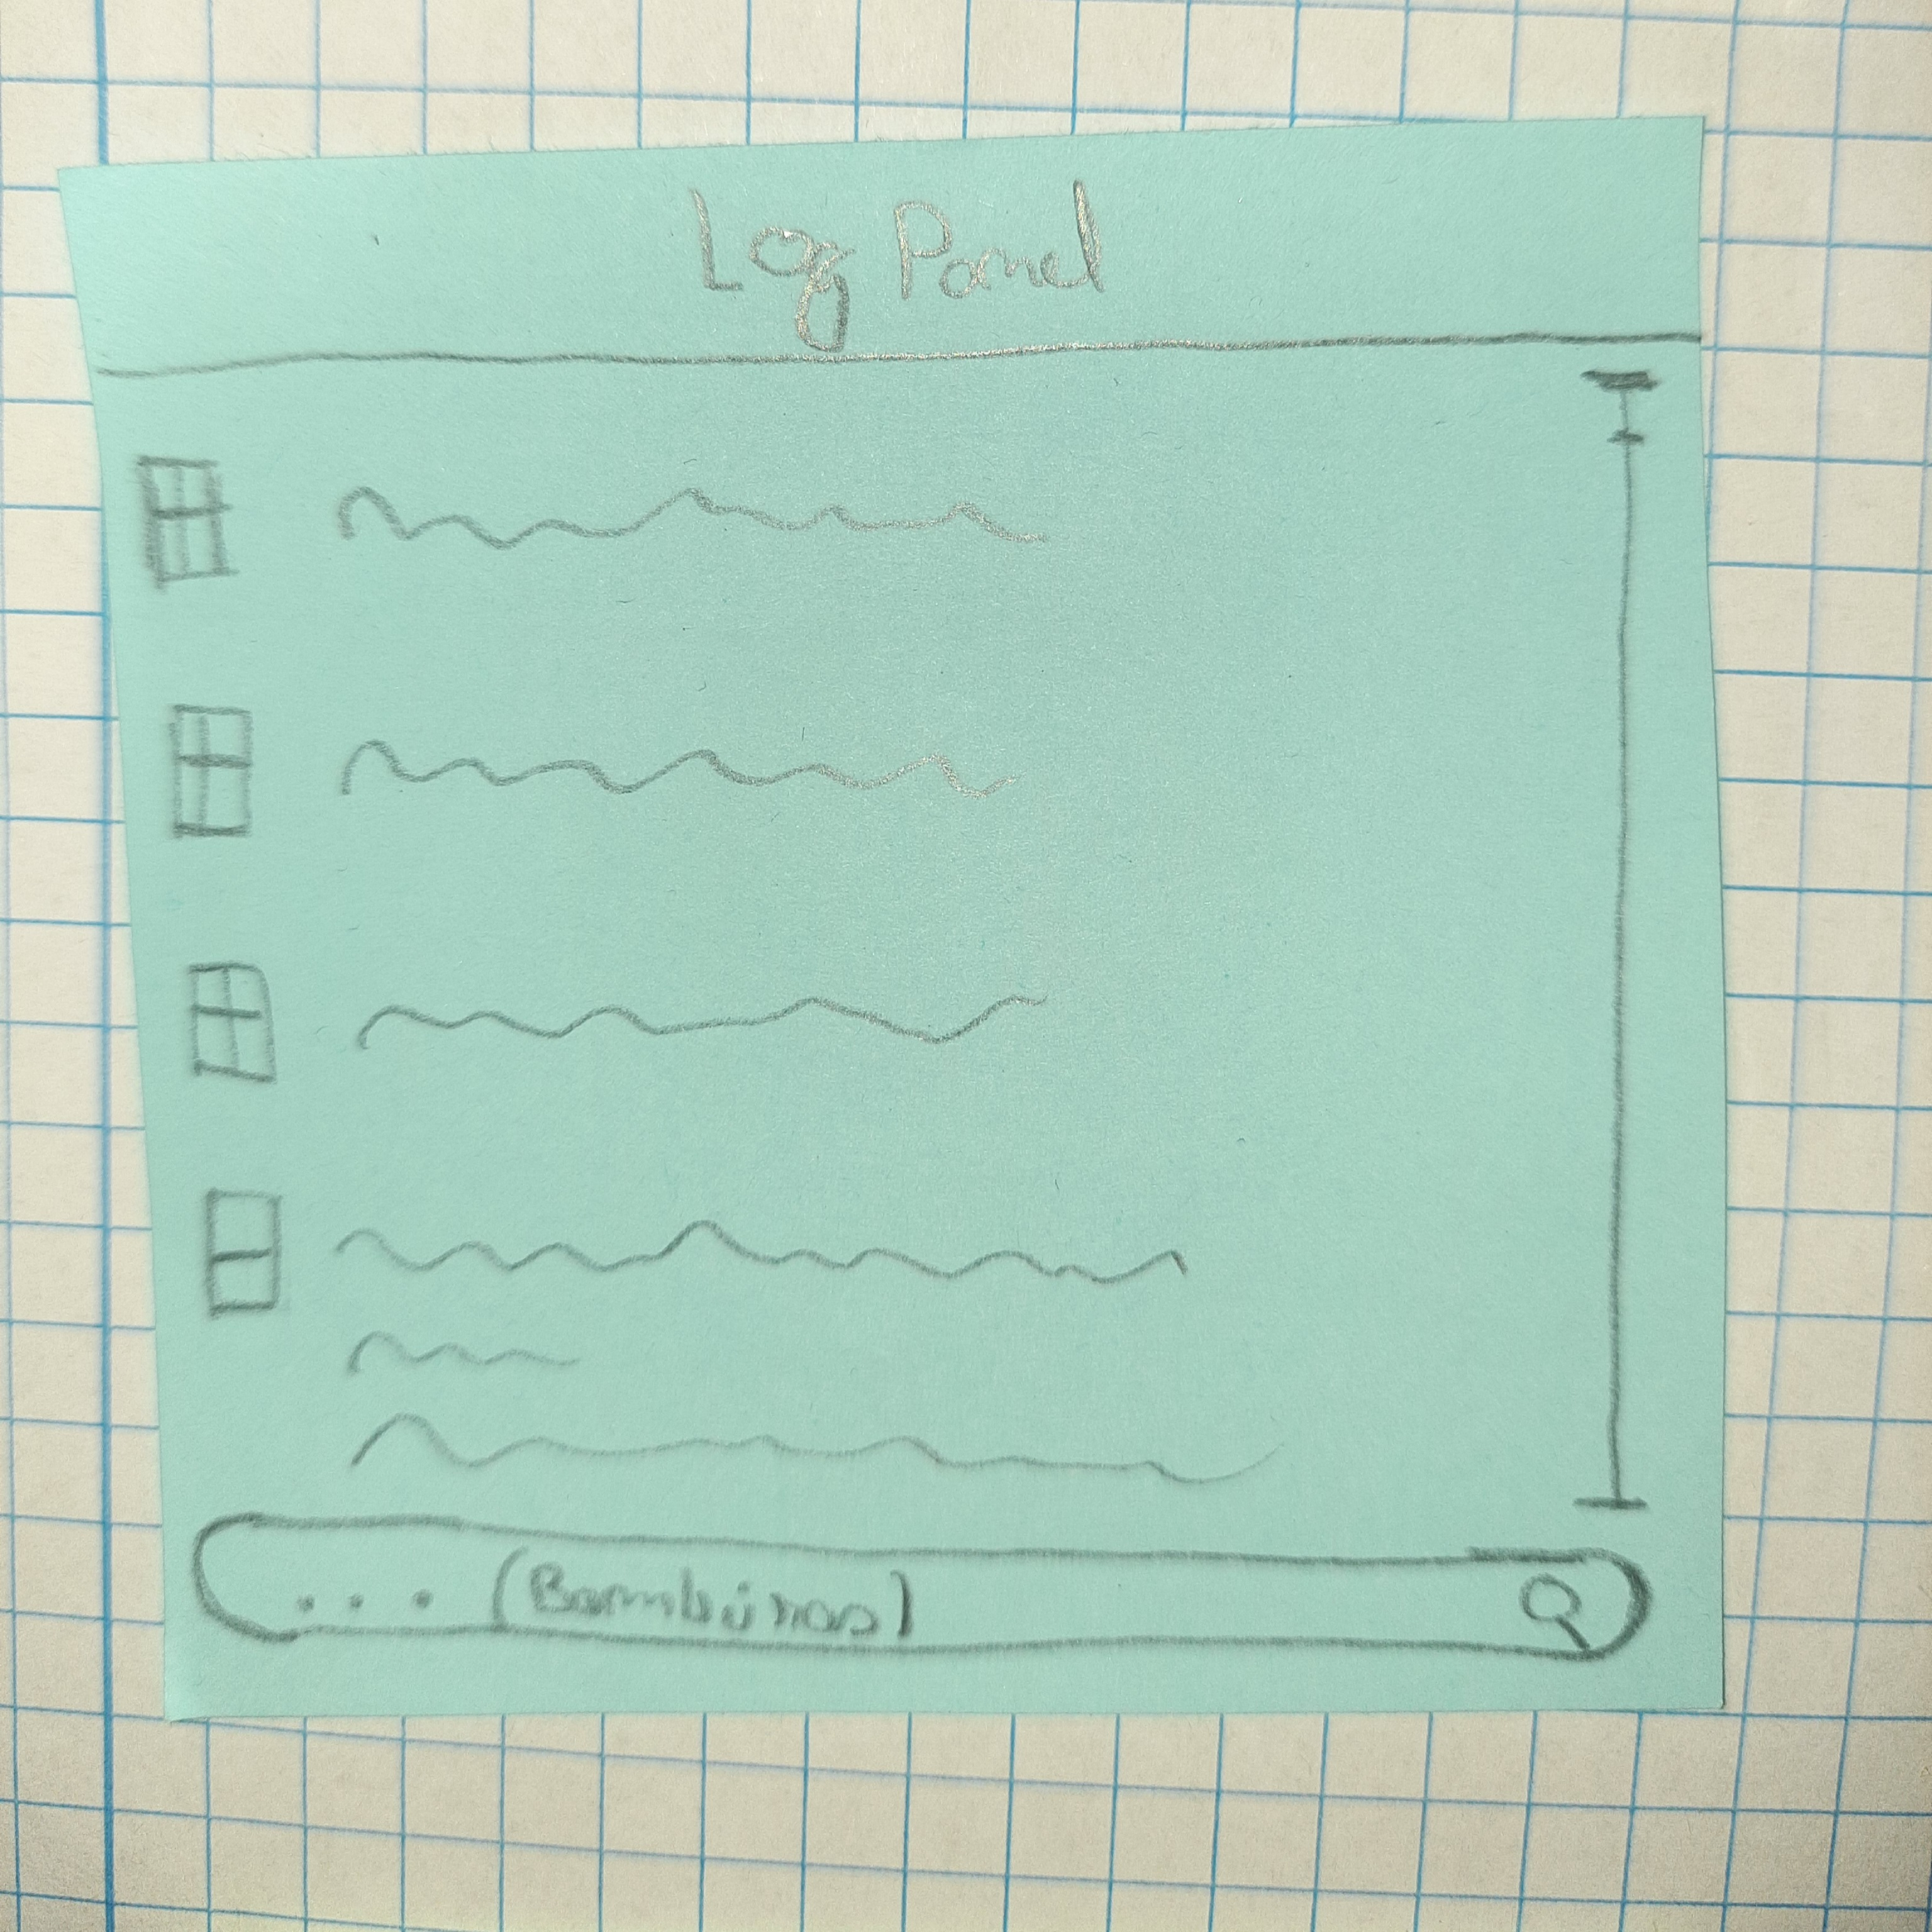
\includegraphics[width=.5\textwidth]{sketches/Log_4.jpg}
            }%
            }
        %\end{figure}
        %\begin{figure}\ContinuedFloat
            \centerline{%
            \subfloat[Sketch 5]{
                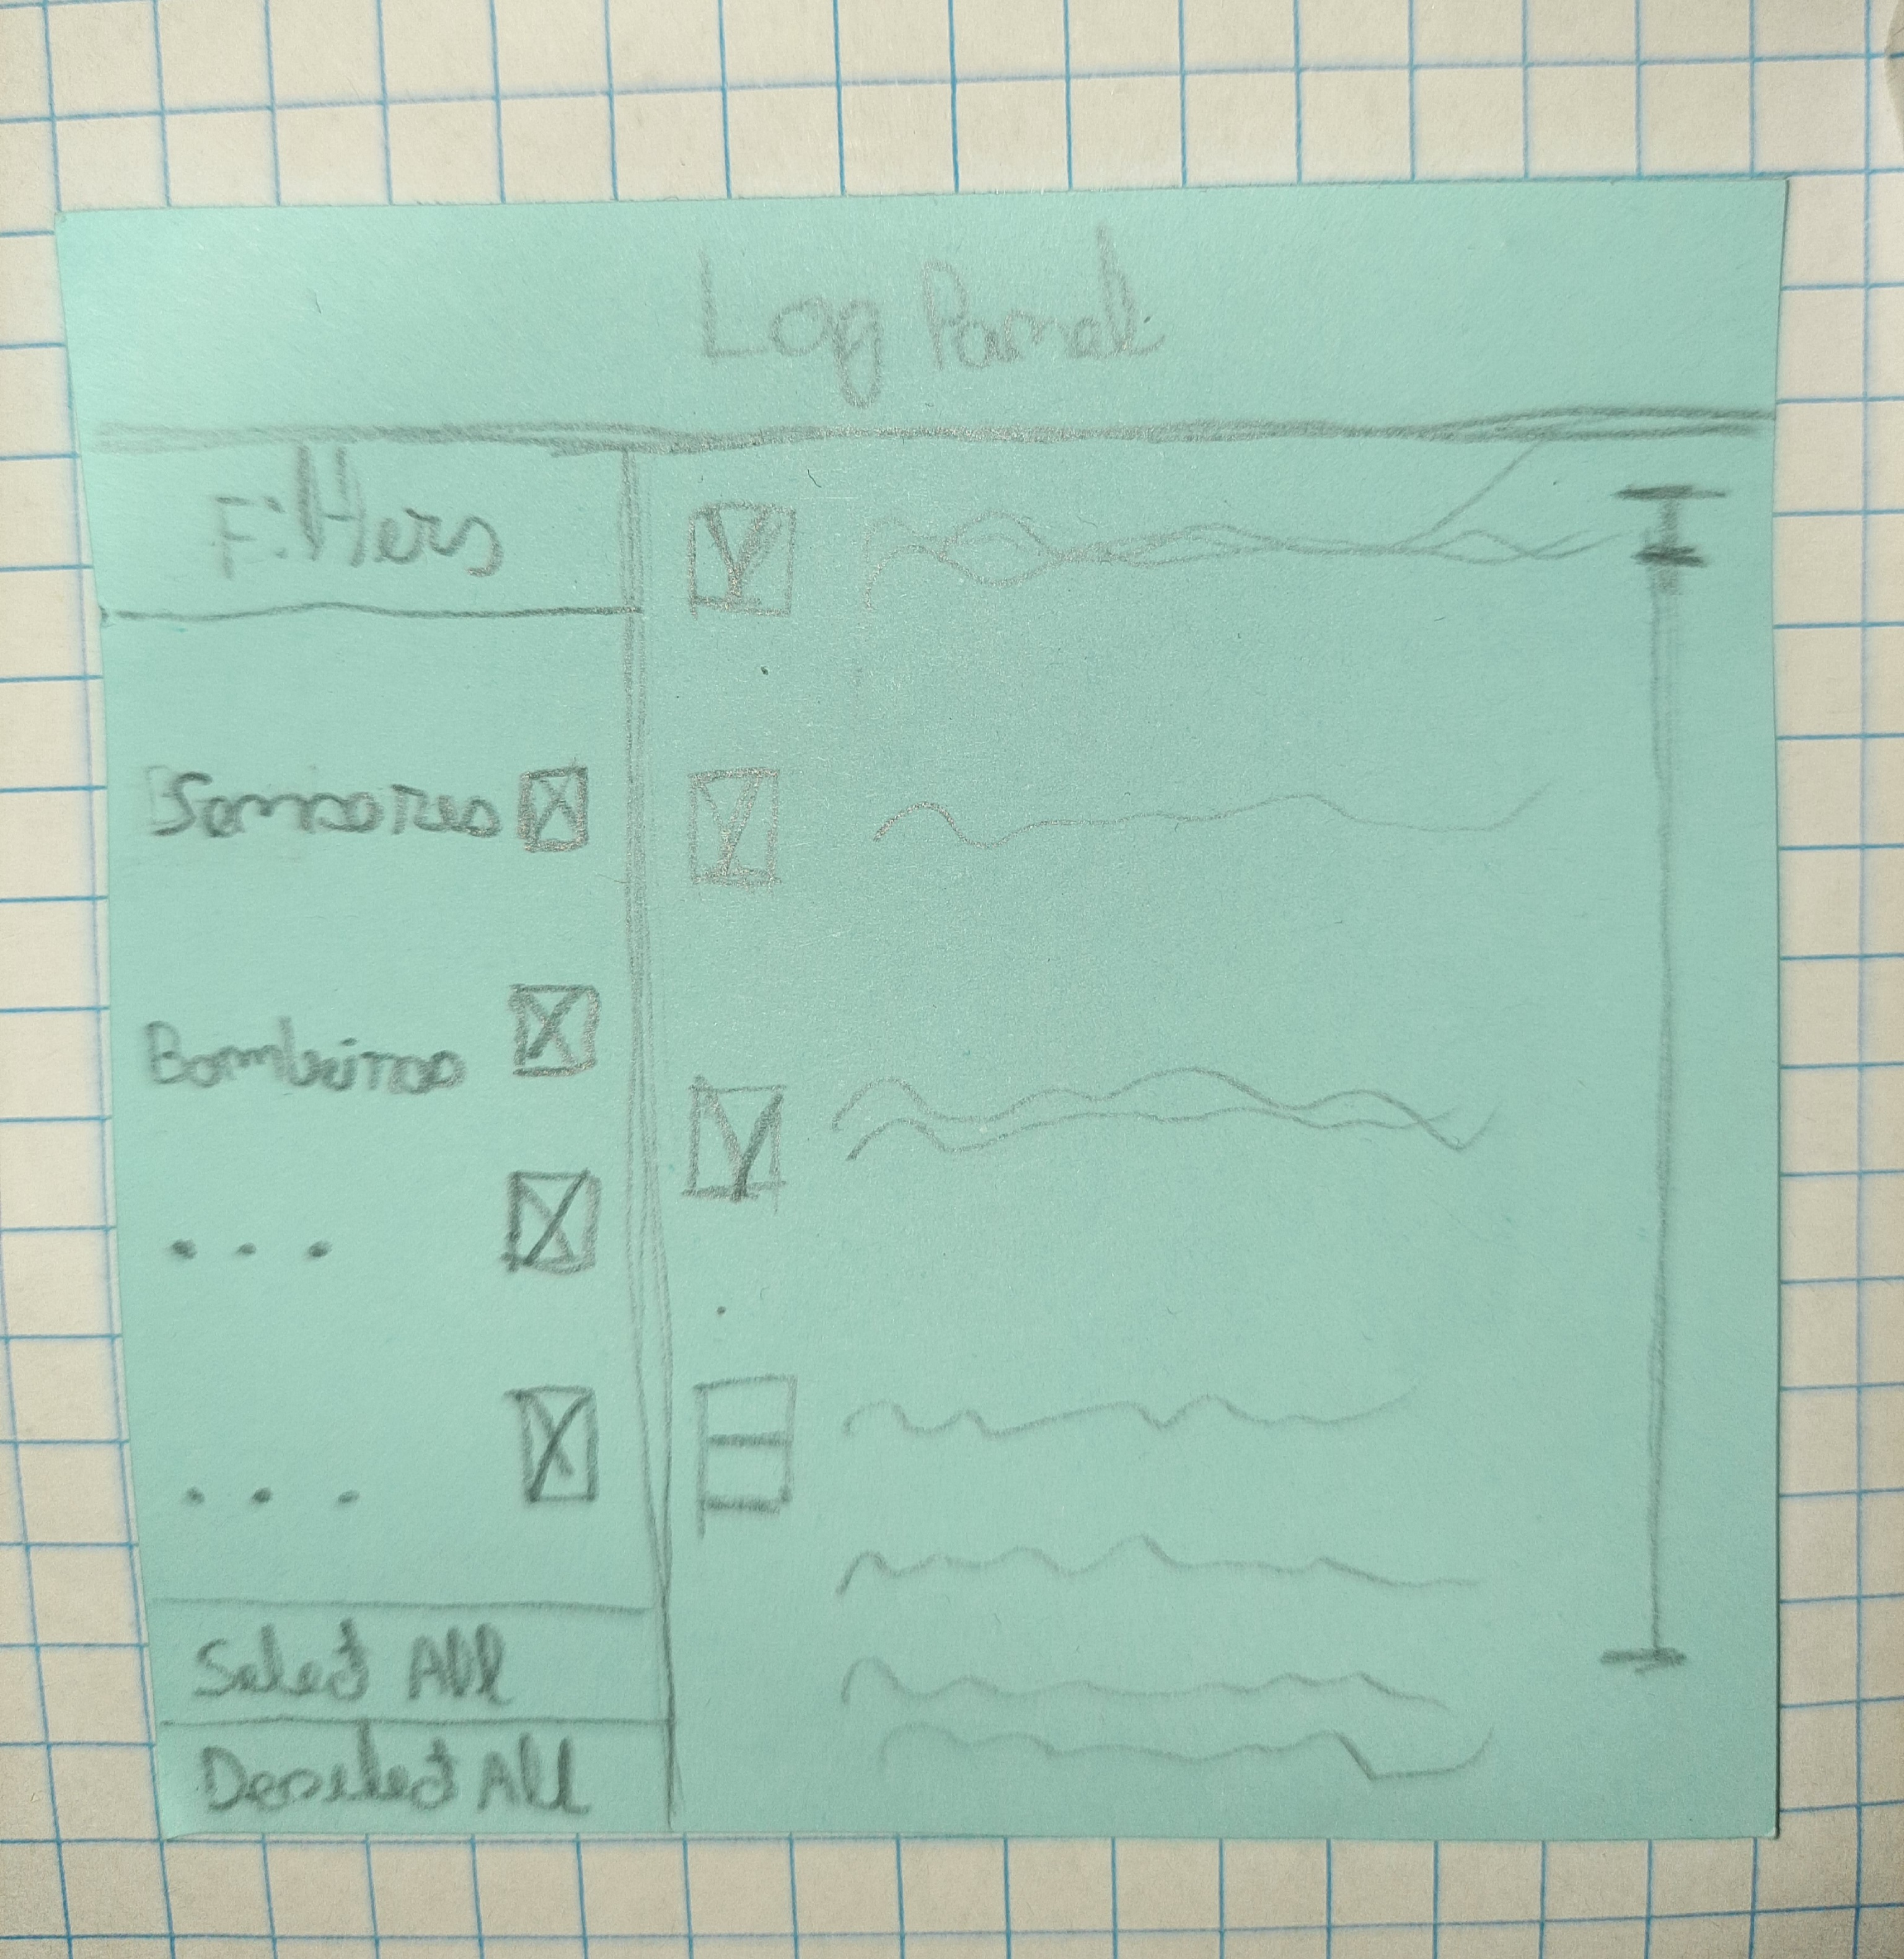
\includegraphics[width=.5\textwidth]{sketches/Log_5.jpg}
            }%
            }
        \caption{Log Panel Sketches}
        \end{figure}
    \item \textbf{Resources Panel:}
        \begin{figure}[H]
            \centerline{%
            \subfloat[Sketch 1]{
                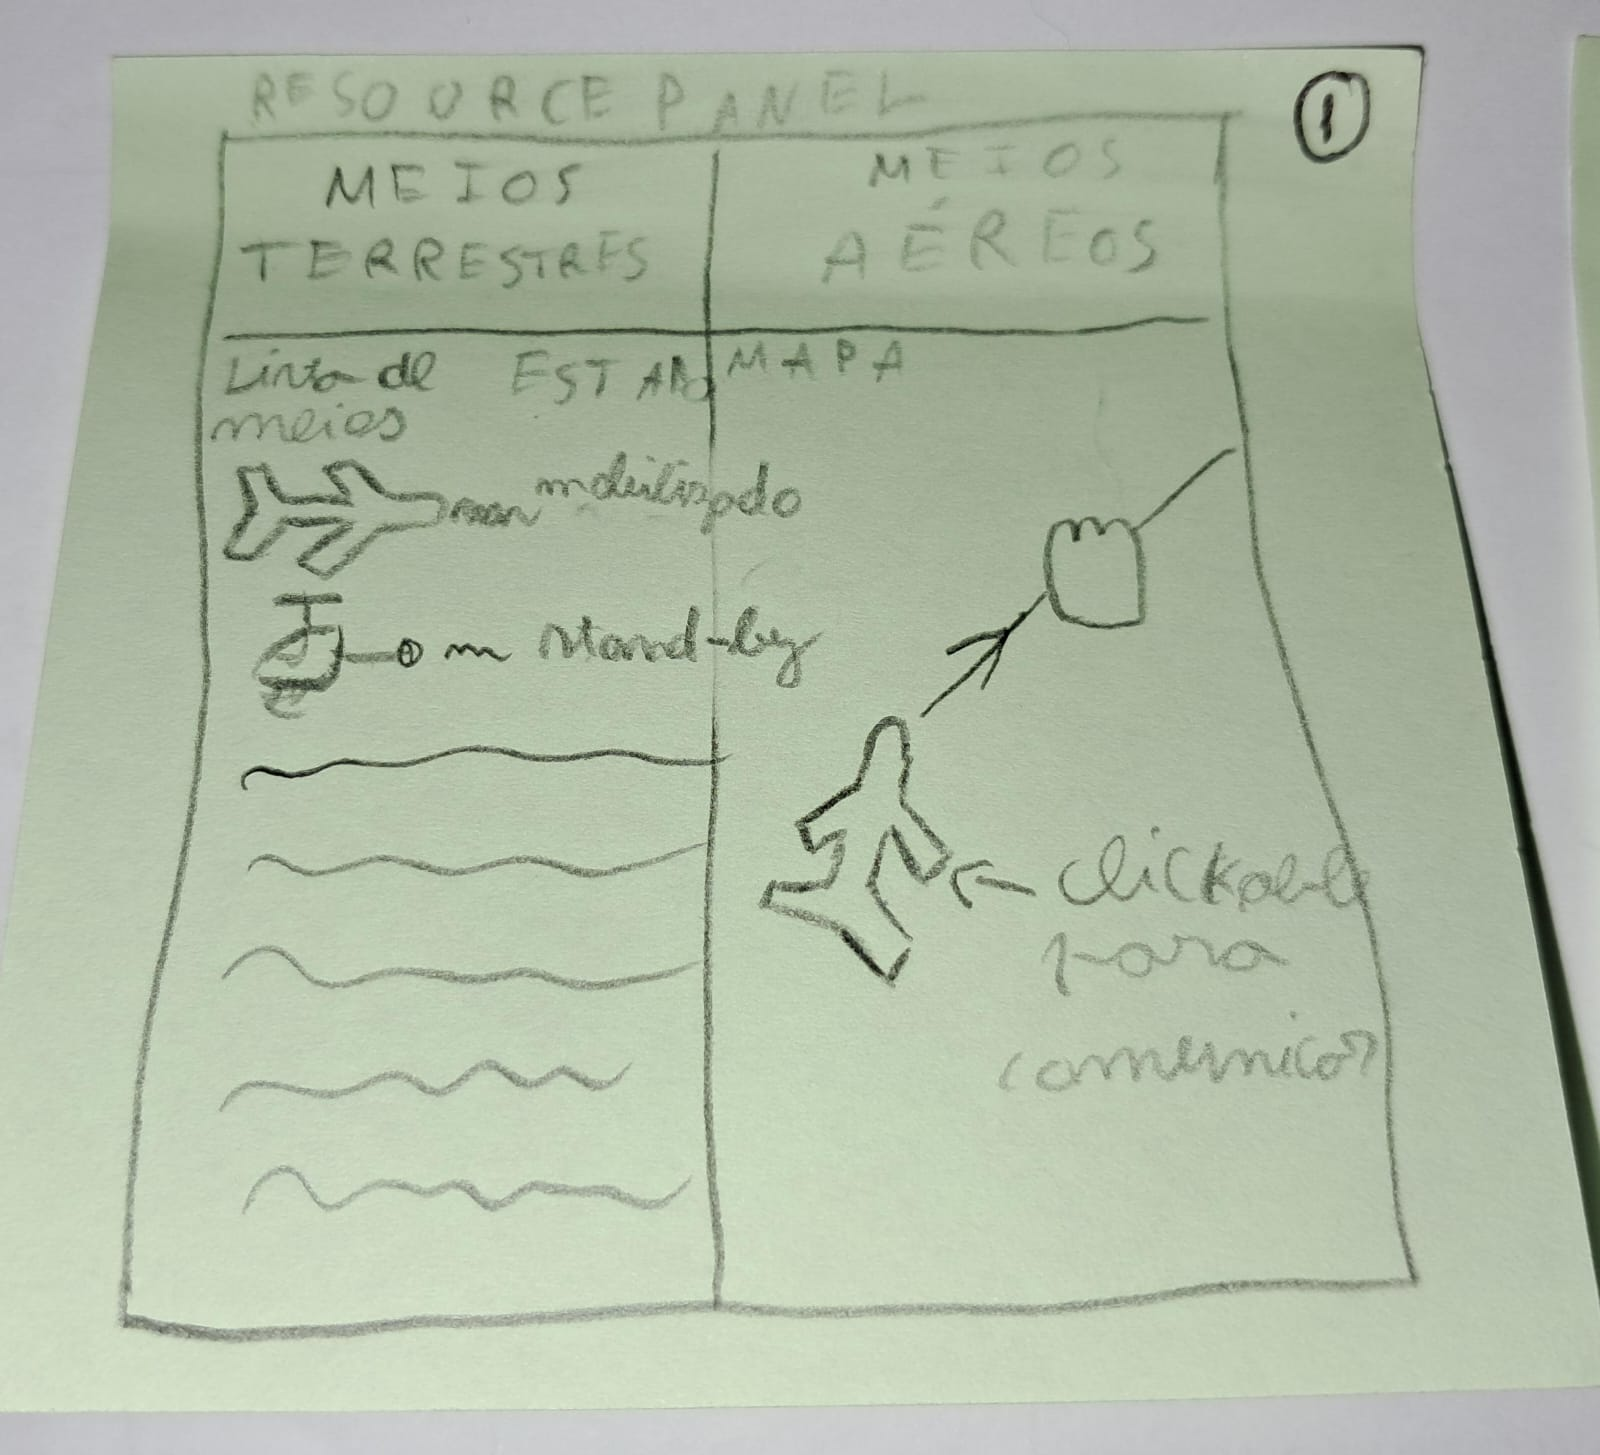
\includegraphics[width=.5\textwidth]{sketches/Resources_1.jpg}
            }\hfill
            \subfloat[Sketch 2]{
                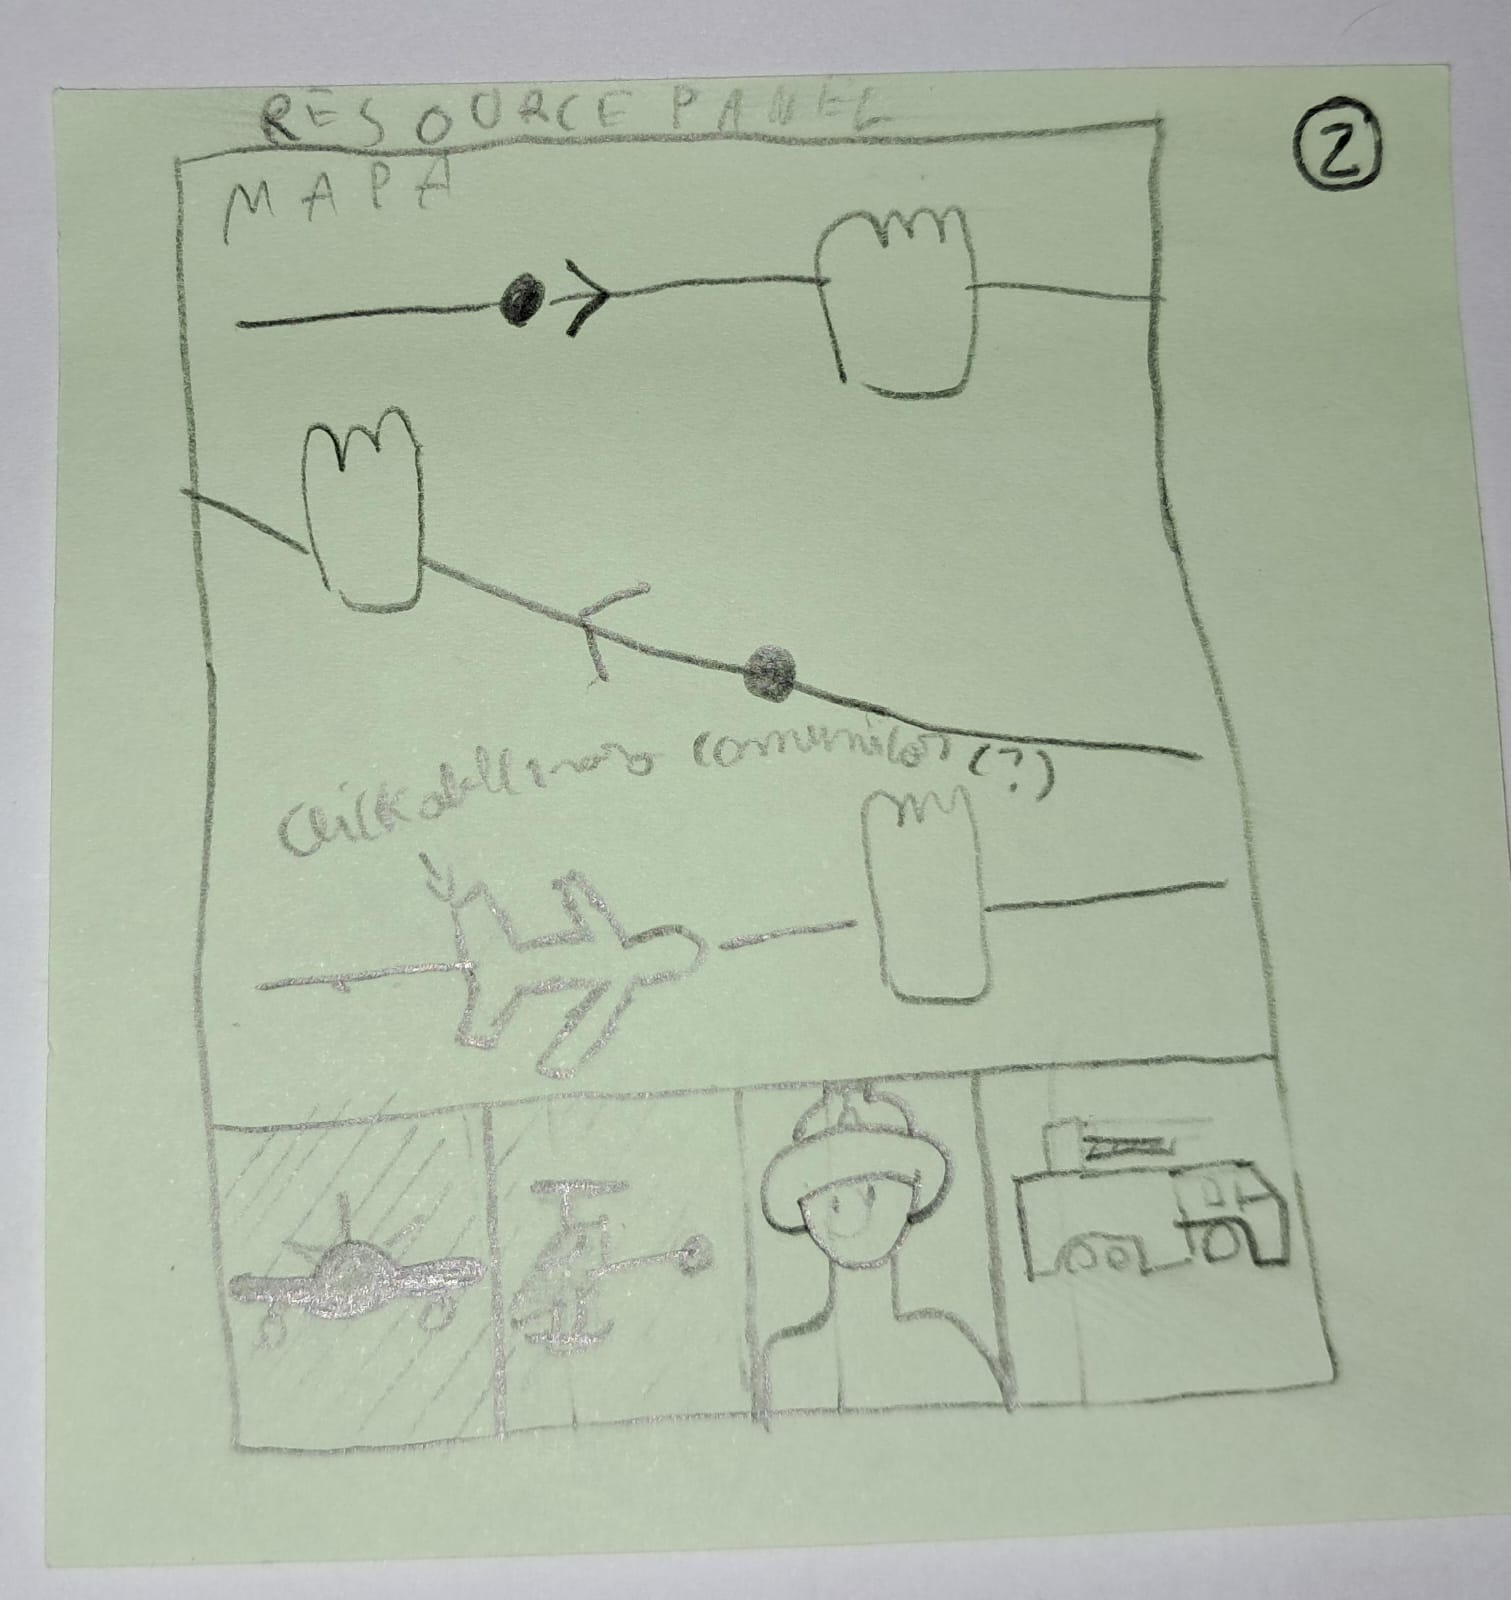
\includegraphics[width=.5\textwidth]{sketches/Resources_2.jpg}
            }%
            }
            \centerline{%
            \subfloat[Sketch 3]{
                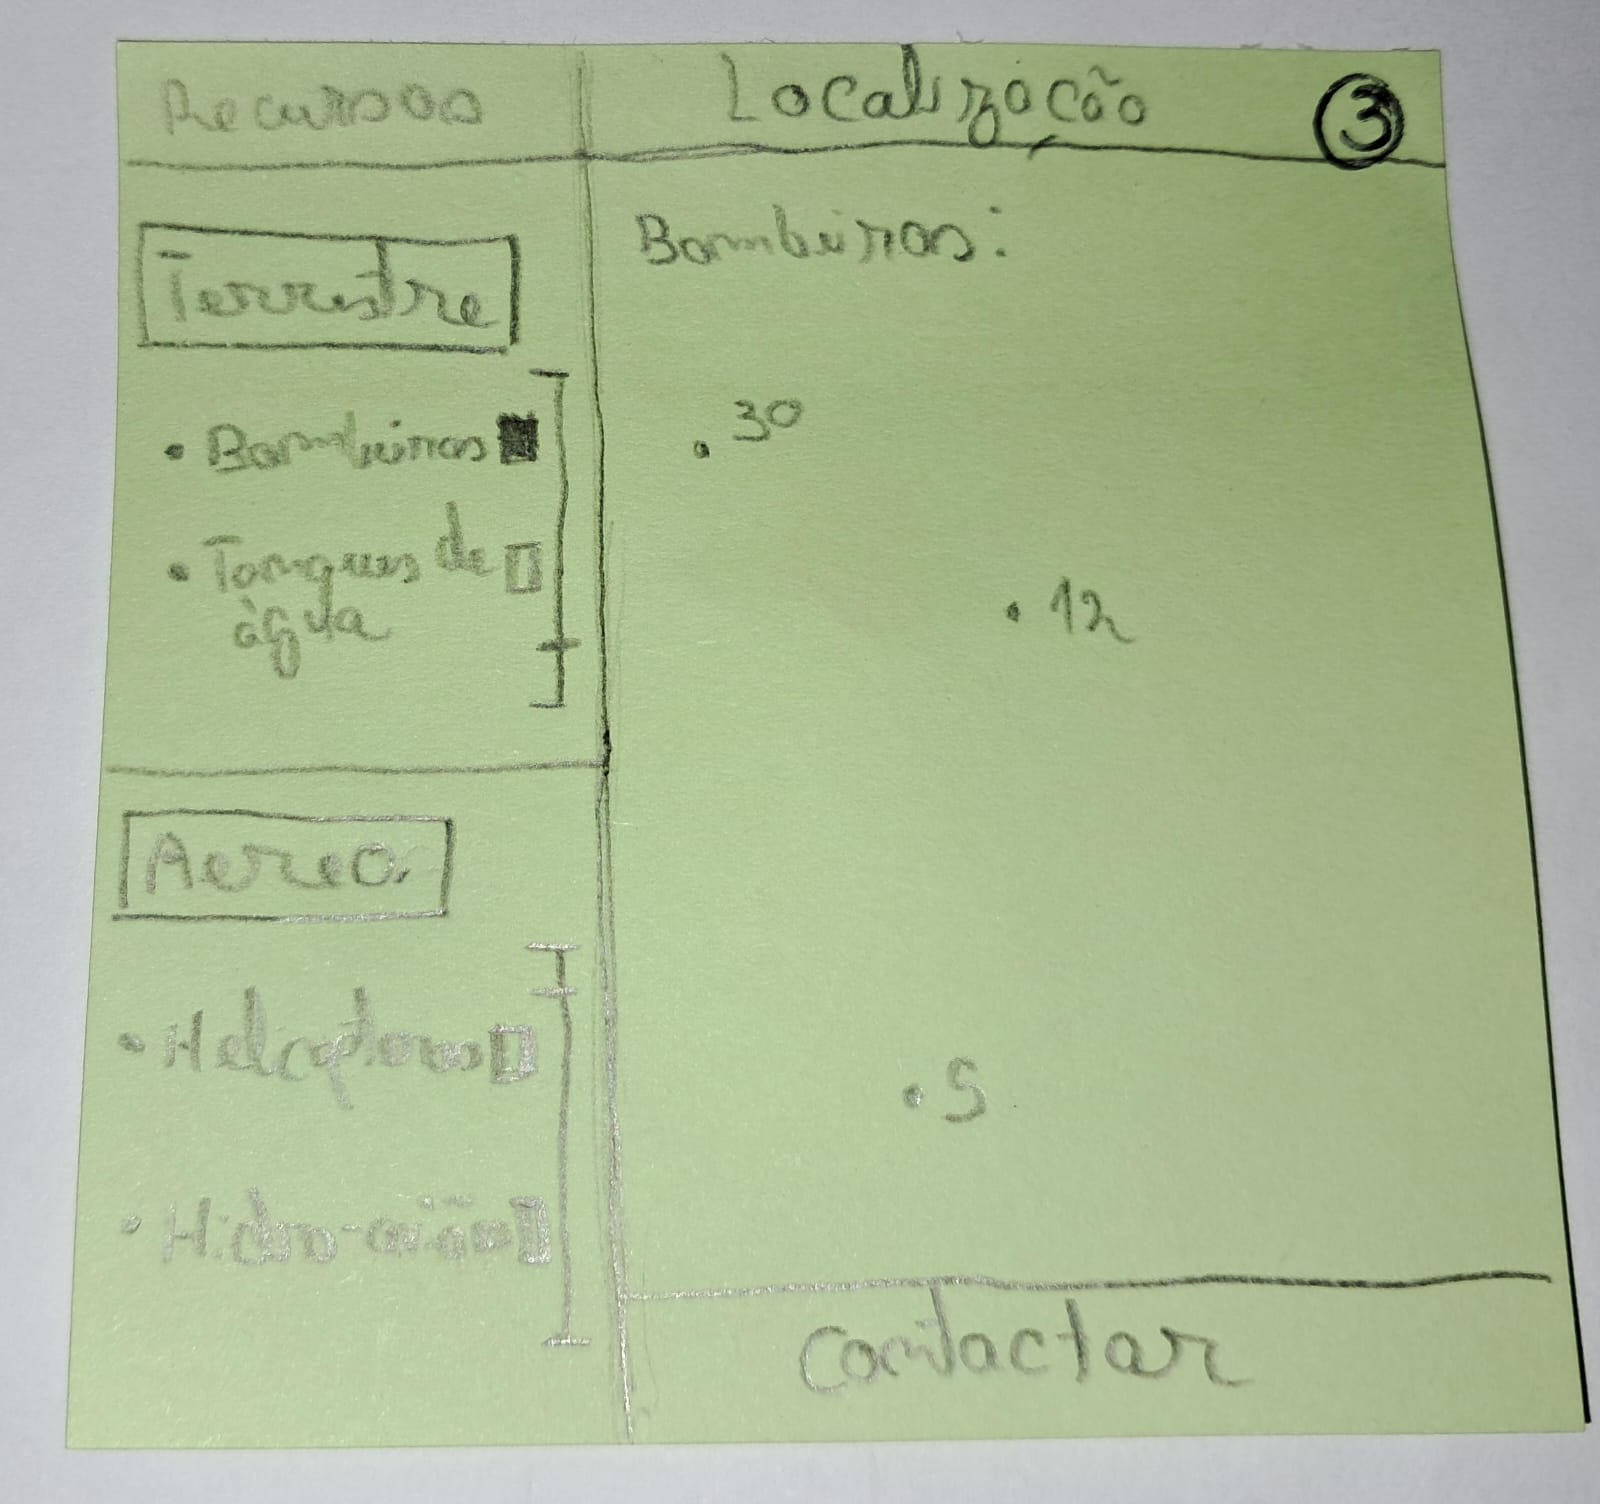
\includegraphics[width=.5\textwidth]{sketches/Resources_3.jpg}
            }\hfill
            \subfloat[Sketch 4]{
                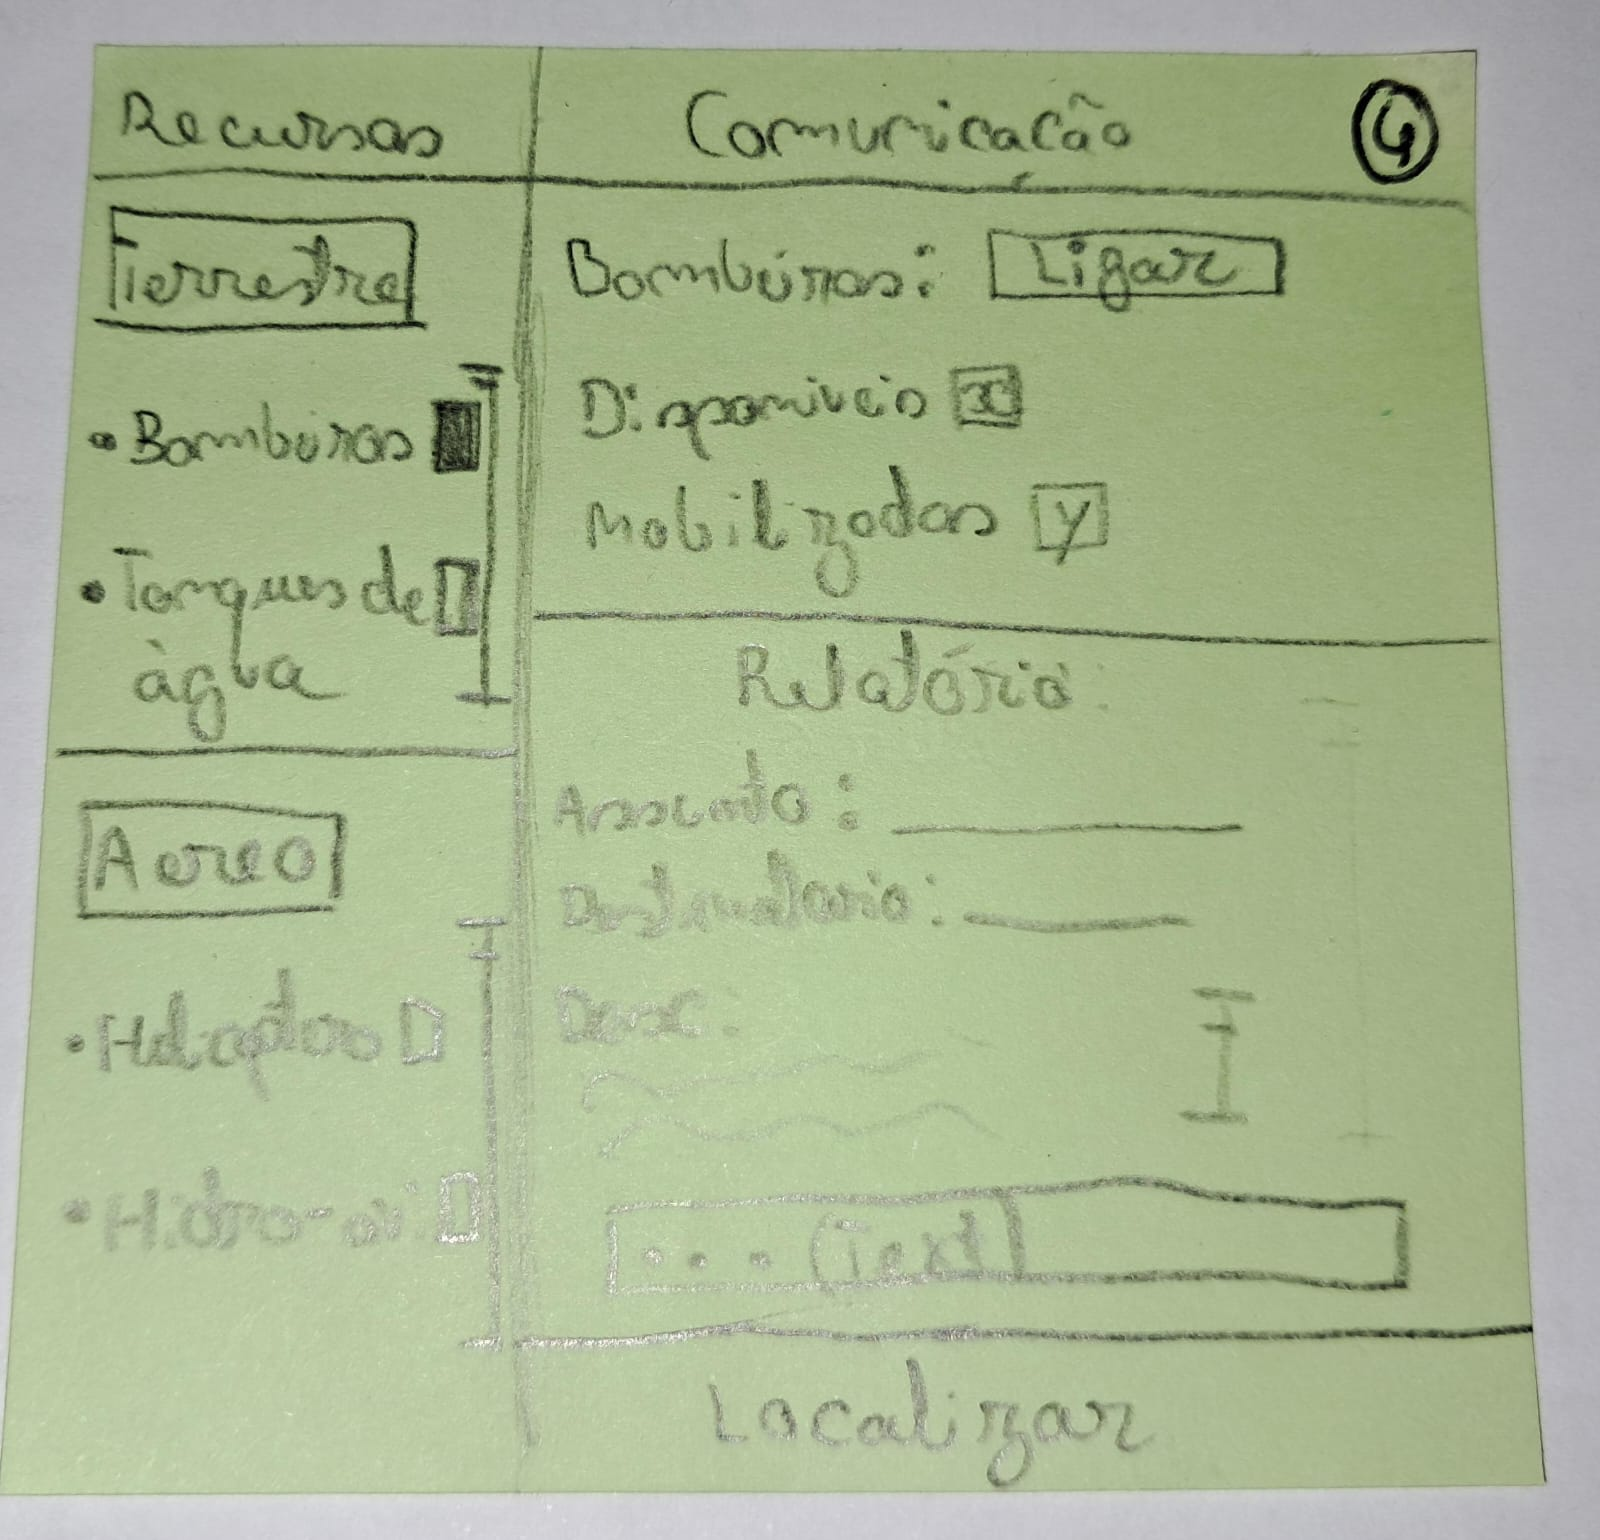
\includegraphics[width=.5\textwidth]{sketches/Resources_4.jpg}
            }%
            }
            \centerline{%
            \subfloat[Sketch 5]{
                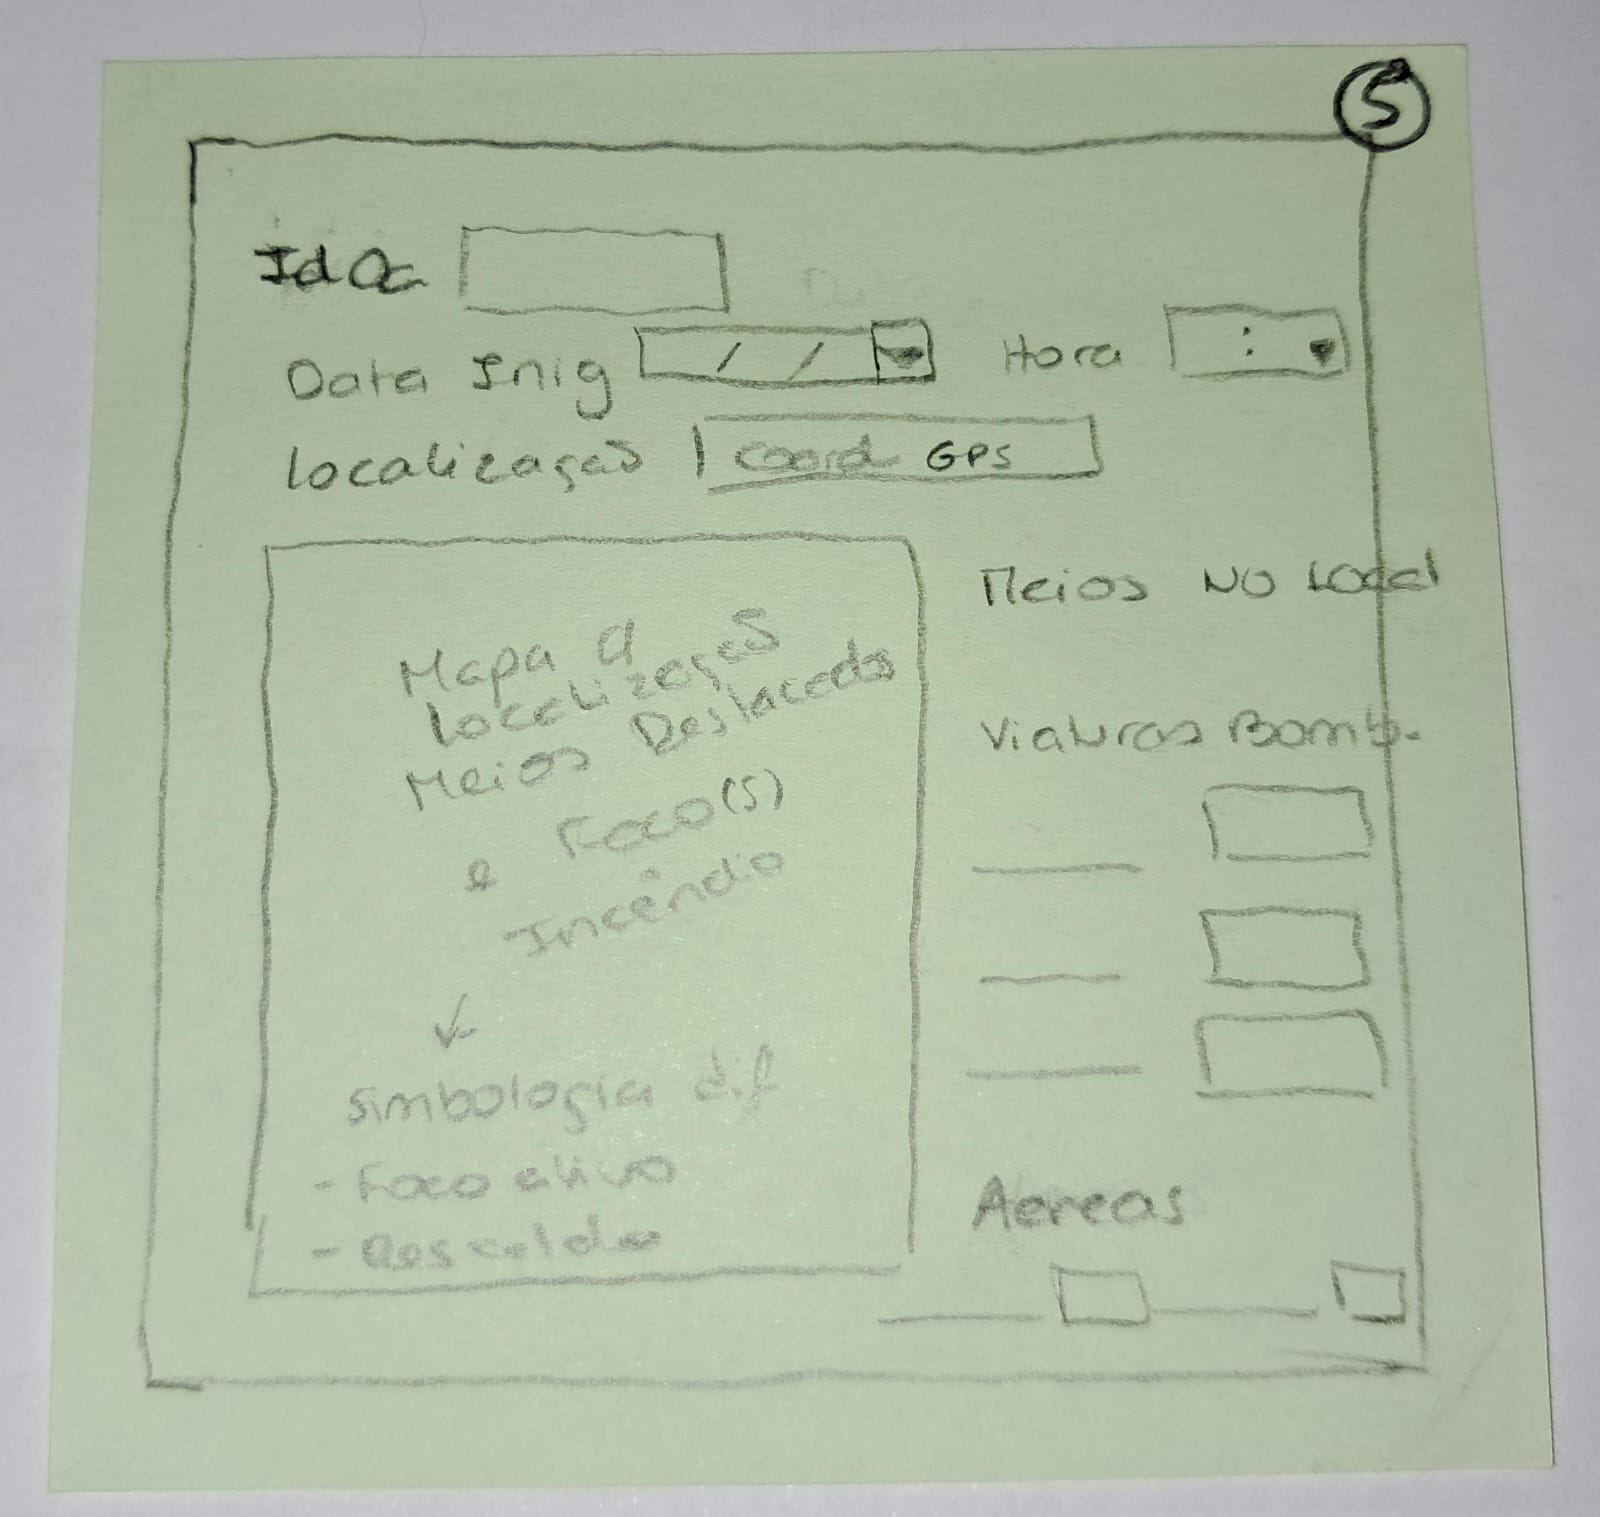
\includegraphics[width=.5\textwidth]{sketches/Resources_5.jpg}
            }\hfill
            \subfloat[Sketch 6]{
                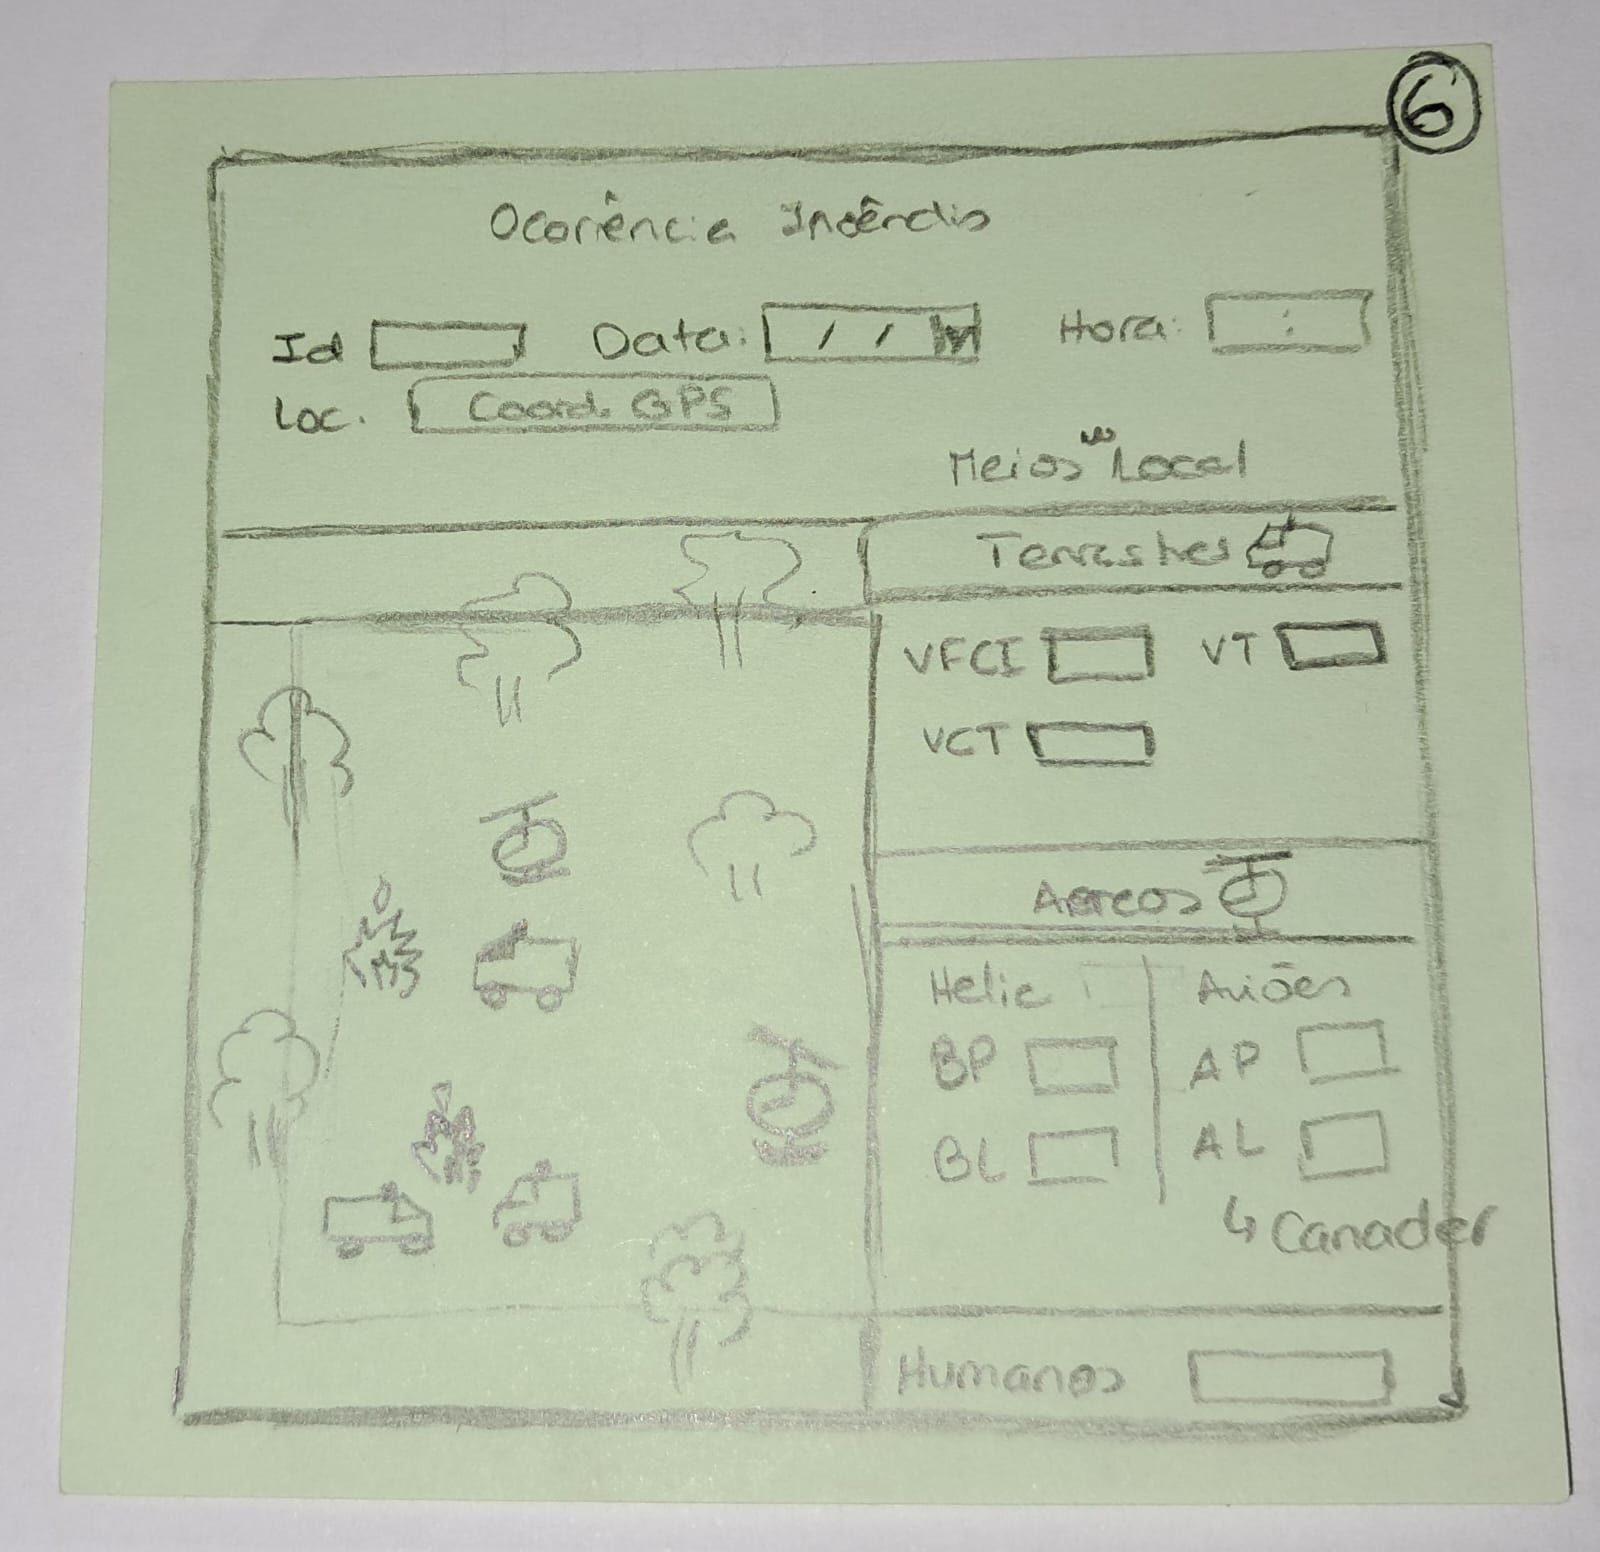
\includegraphics[width=.5\textwidth]{sketches/Resources_6.jpg}
            }%
            }
        \end{figure}
        \begin{figure}[H]\ContinuedFloat
            \centerline{%
            \subfloat[Sketch 7]{
                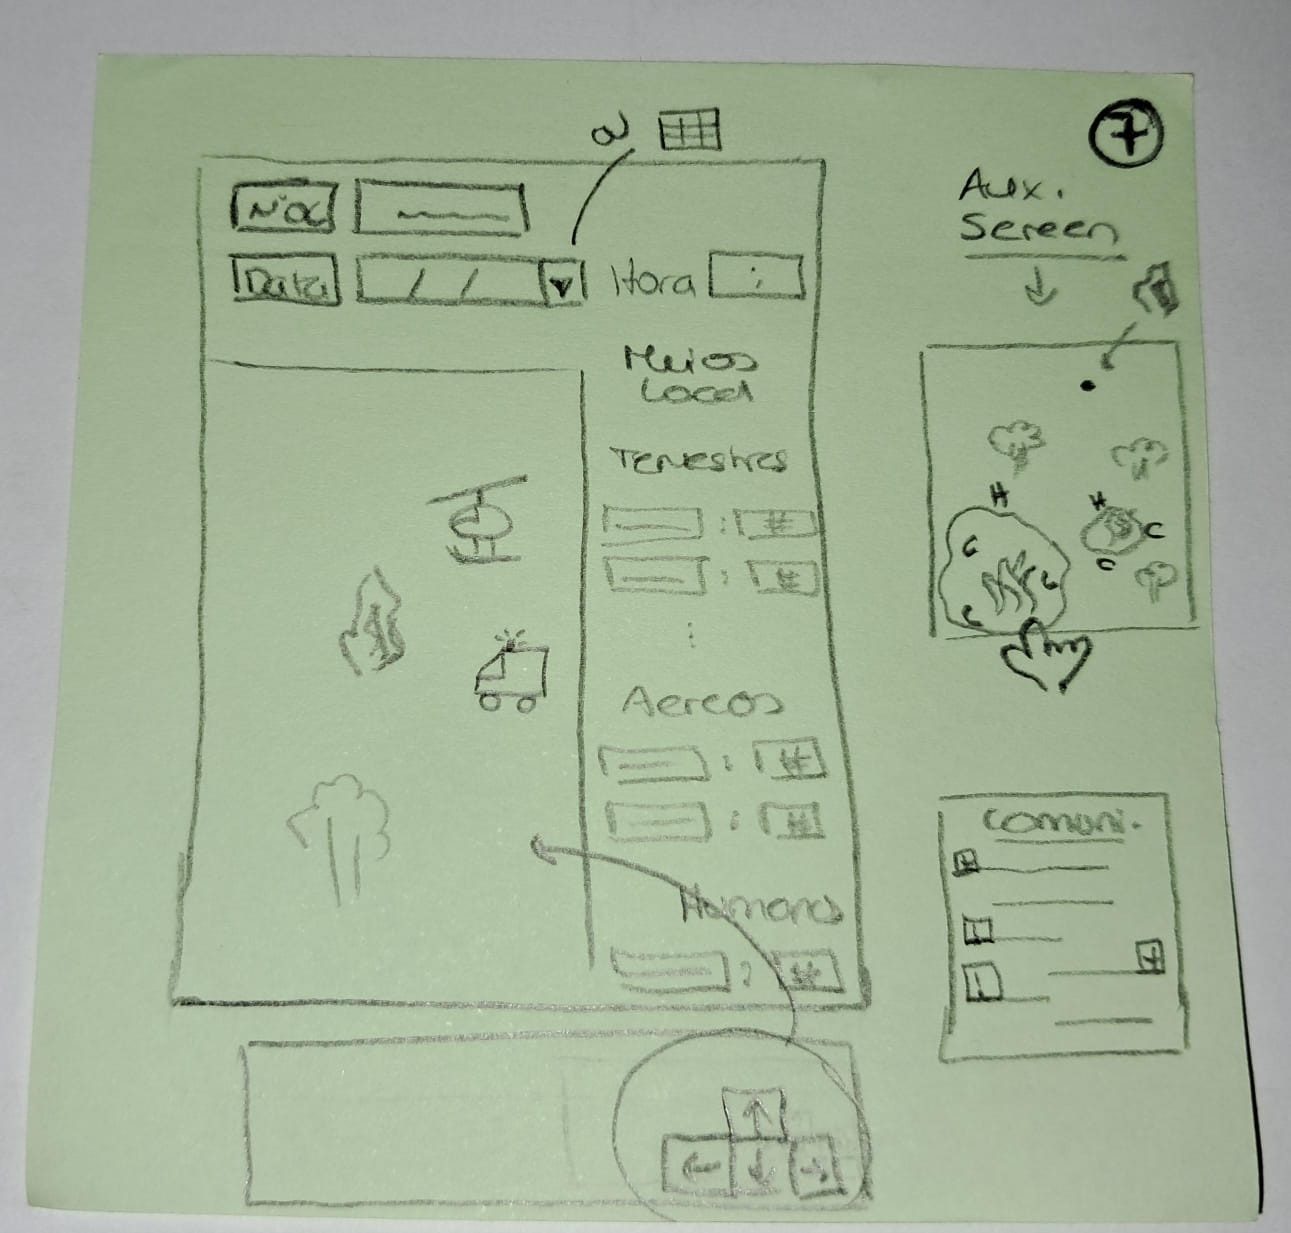
\includegraphics[width=.5\textwidth]{sketches/Resources_7.jpg}
            }%
            }
            \centerline{%
            \subfloat[Sketch 8a]{
                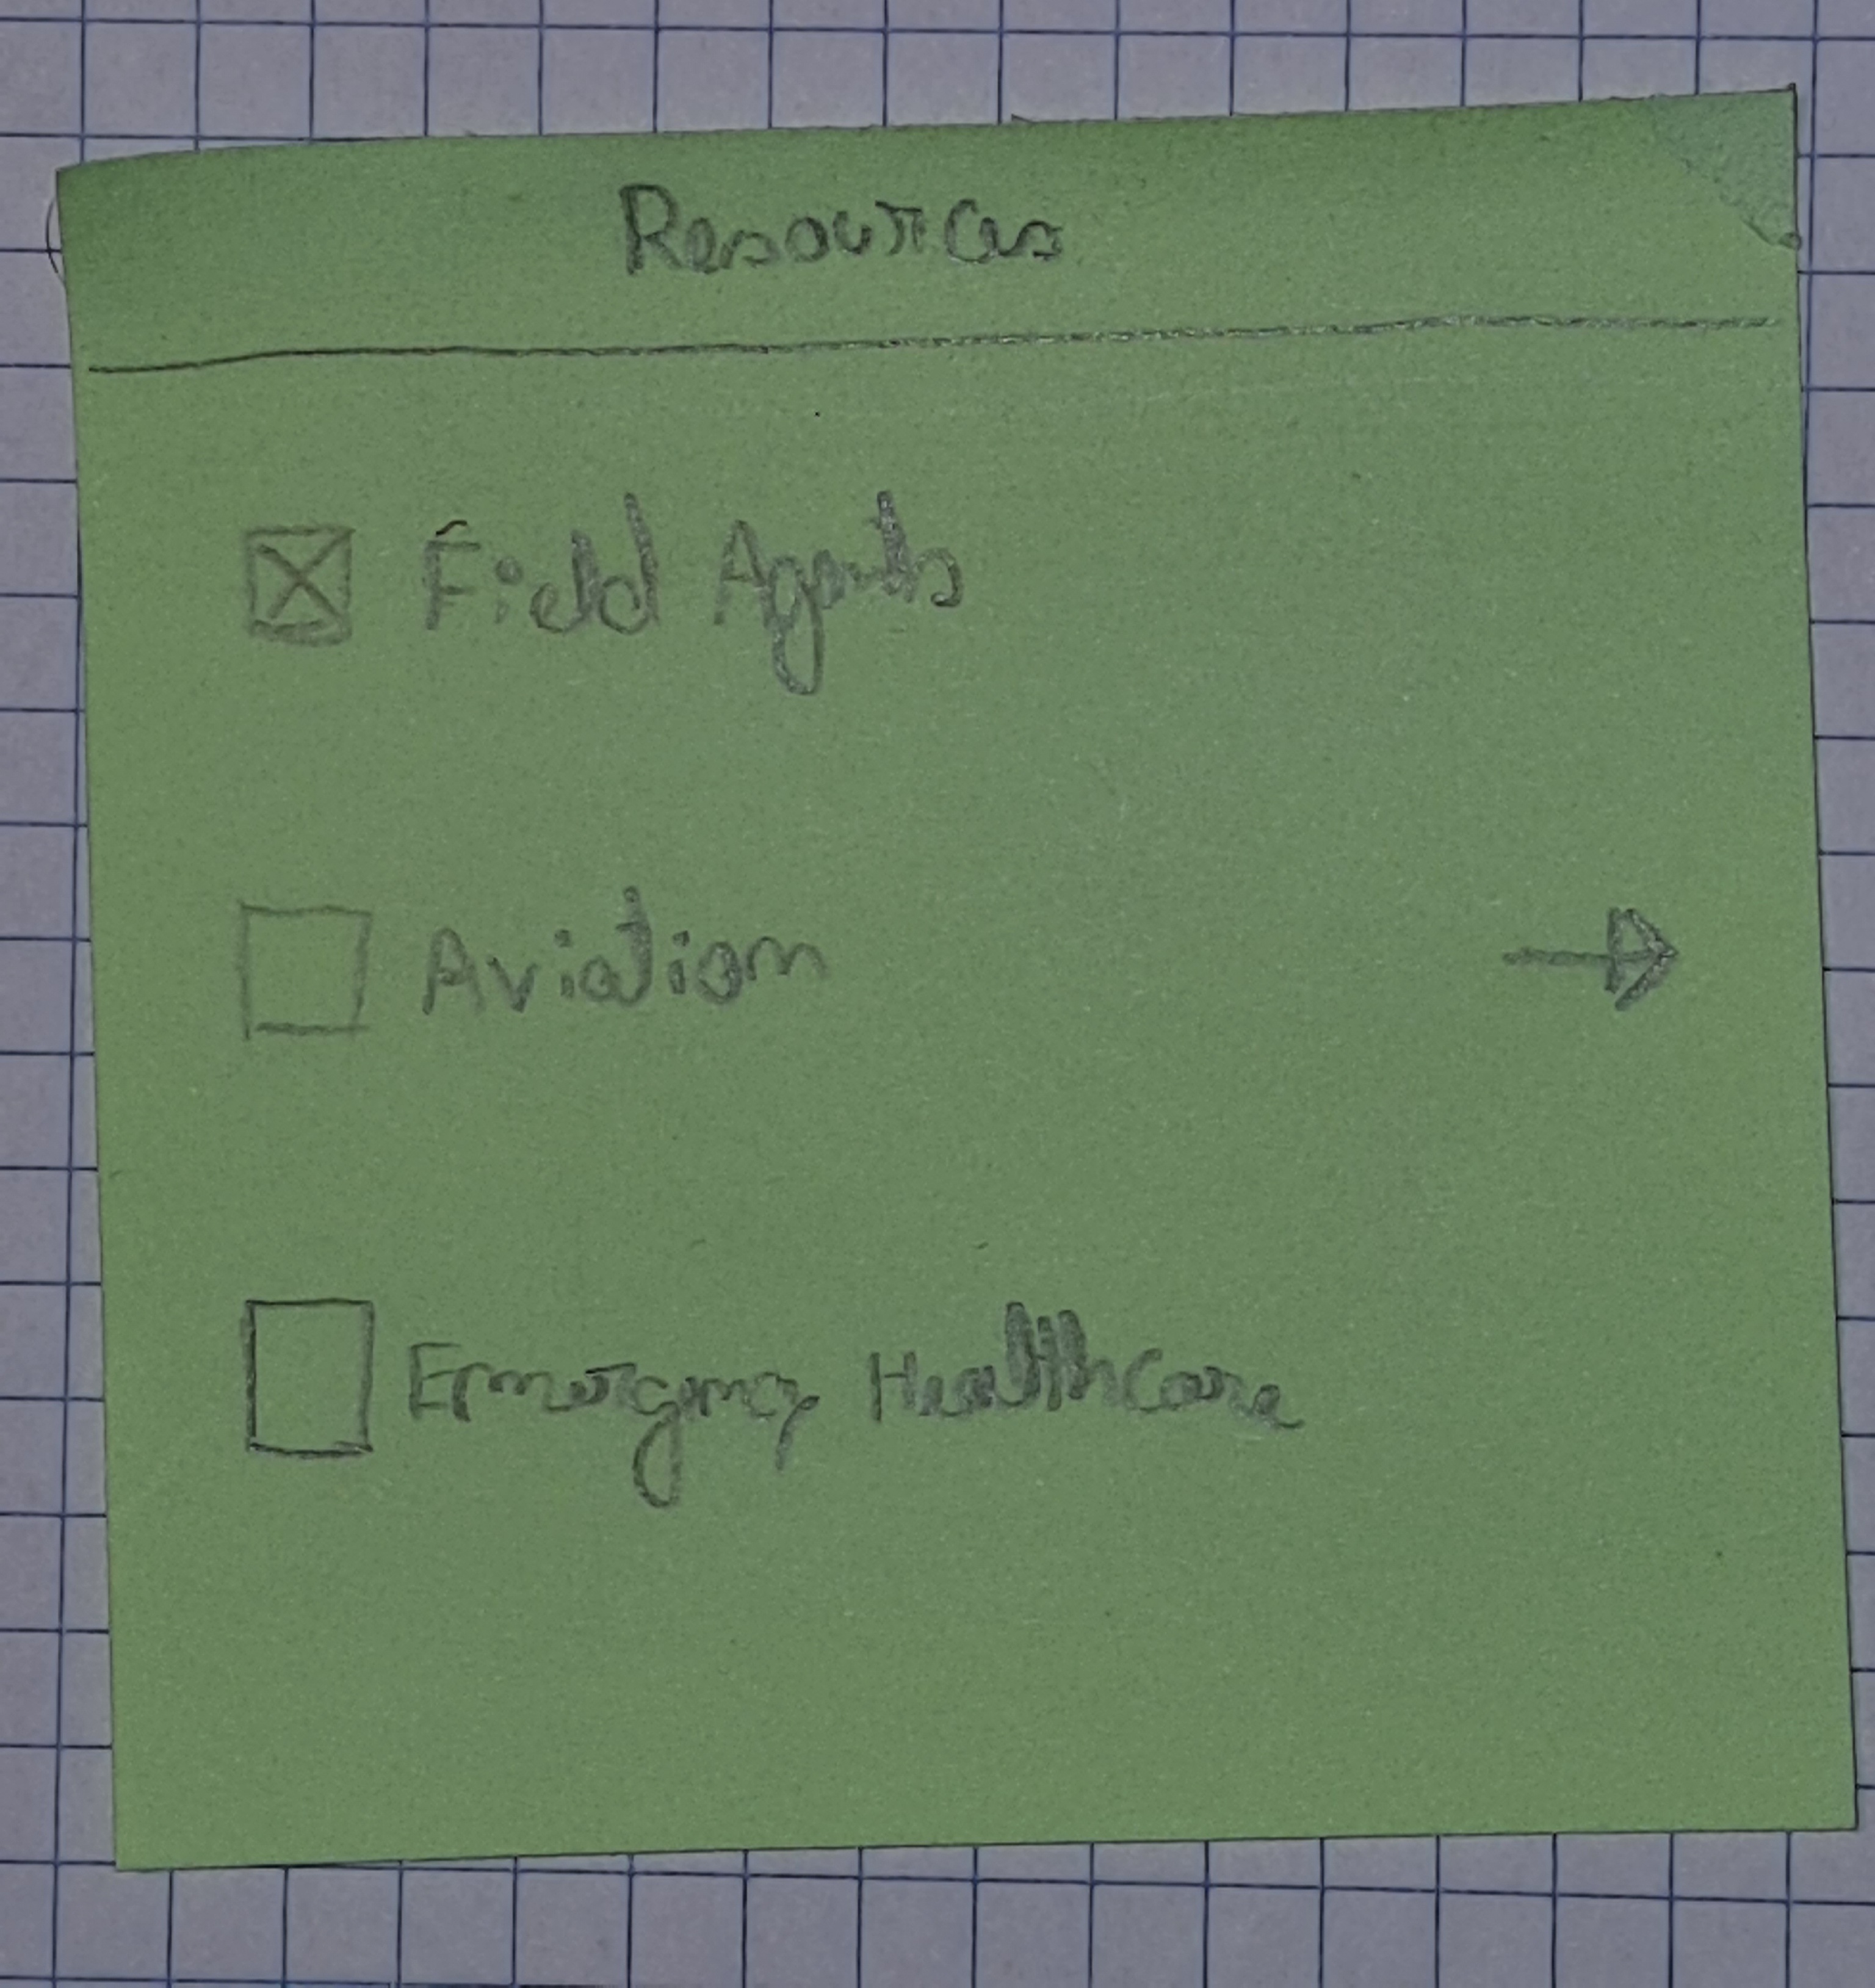
\includegraphics[width=.45\textwidth]{sketches/Resources_8(1).jpg}
            }%
            \subfloat[Sketch 8b]{
                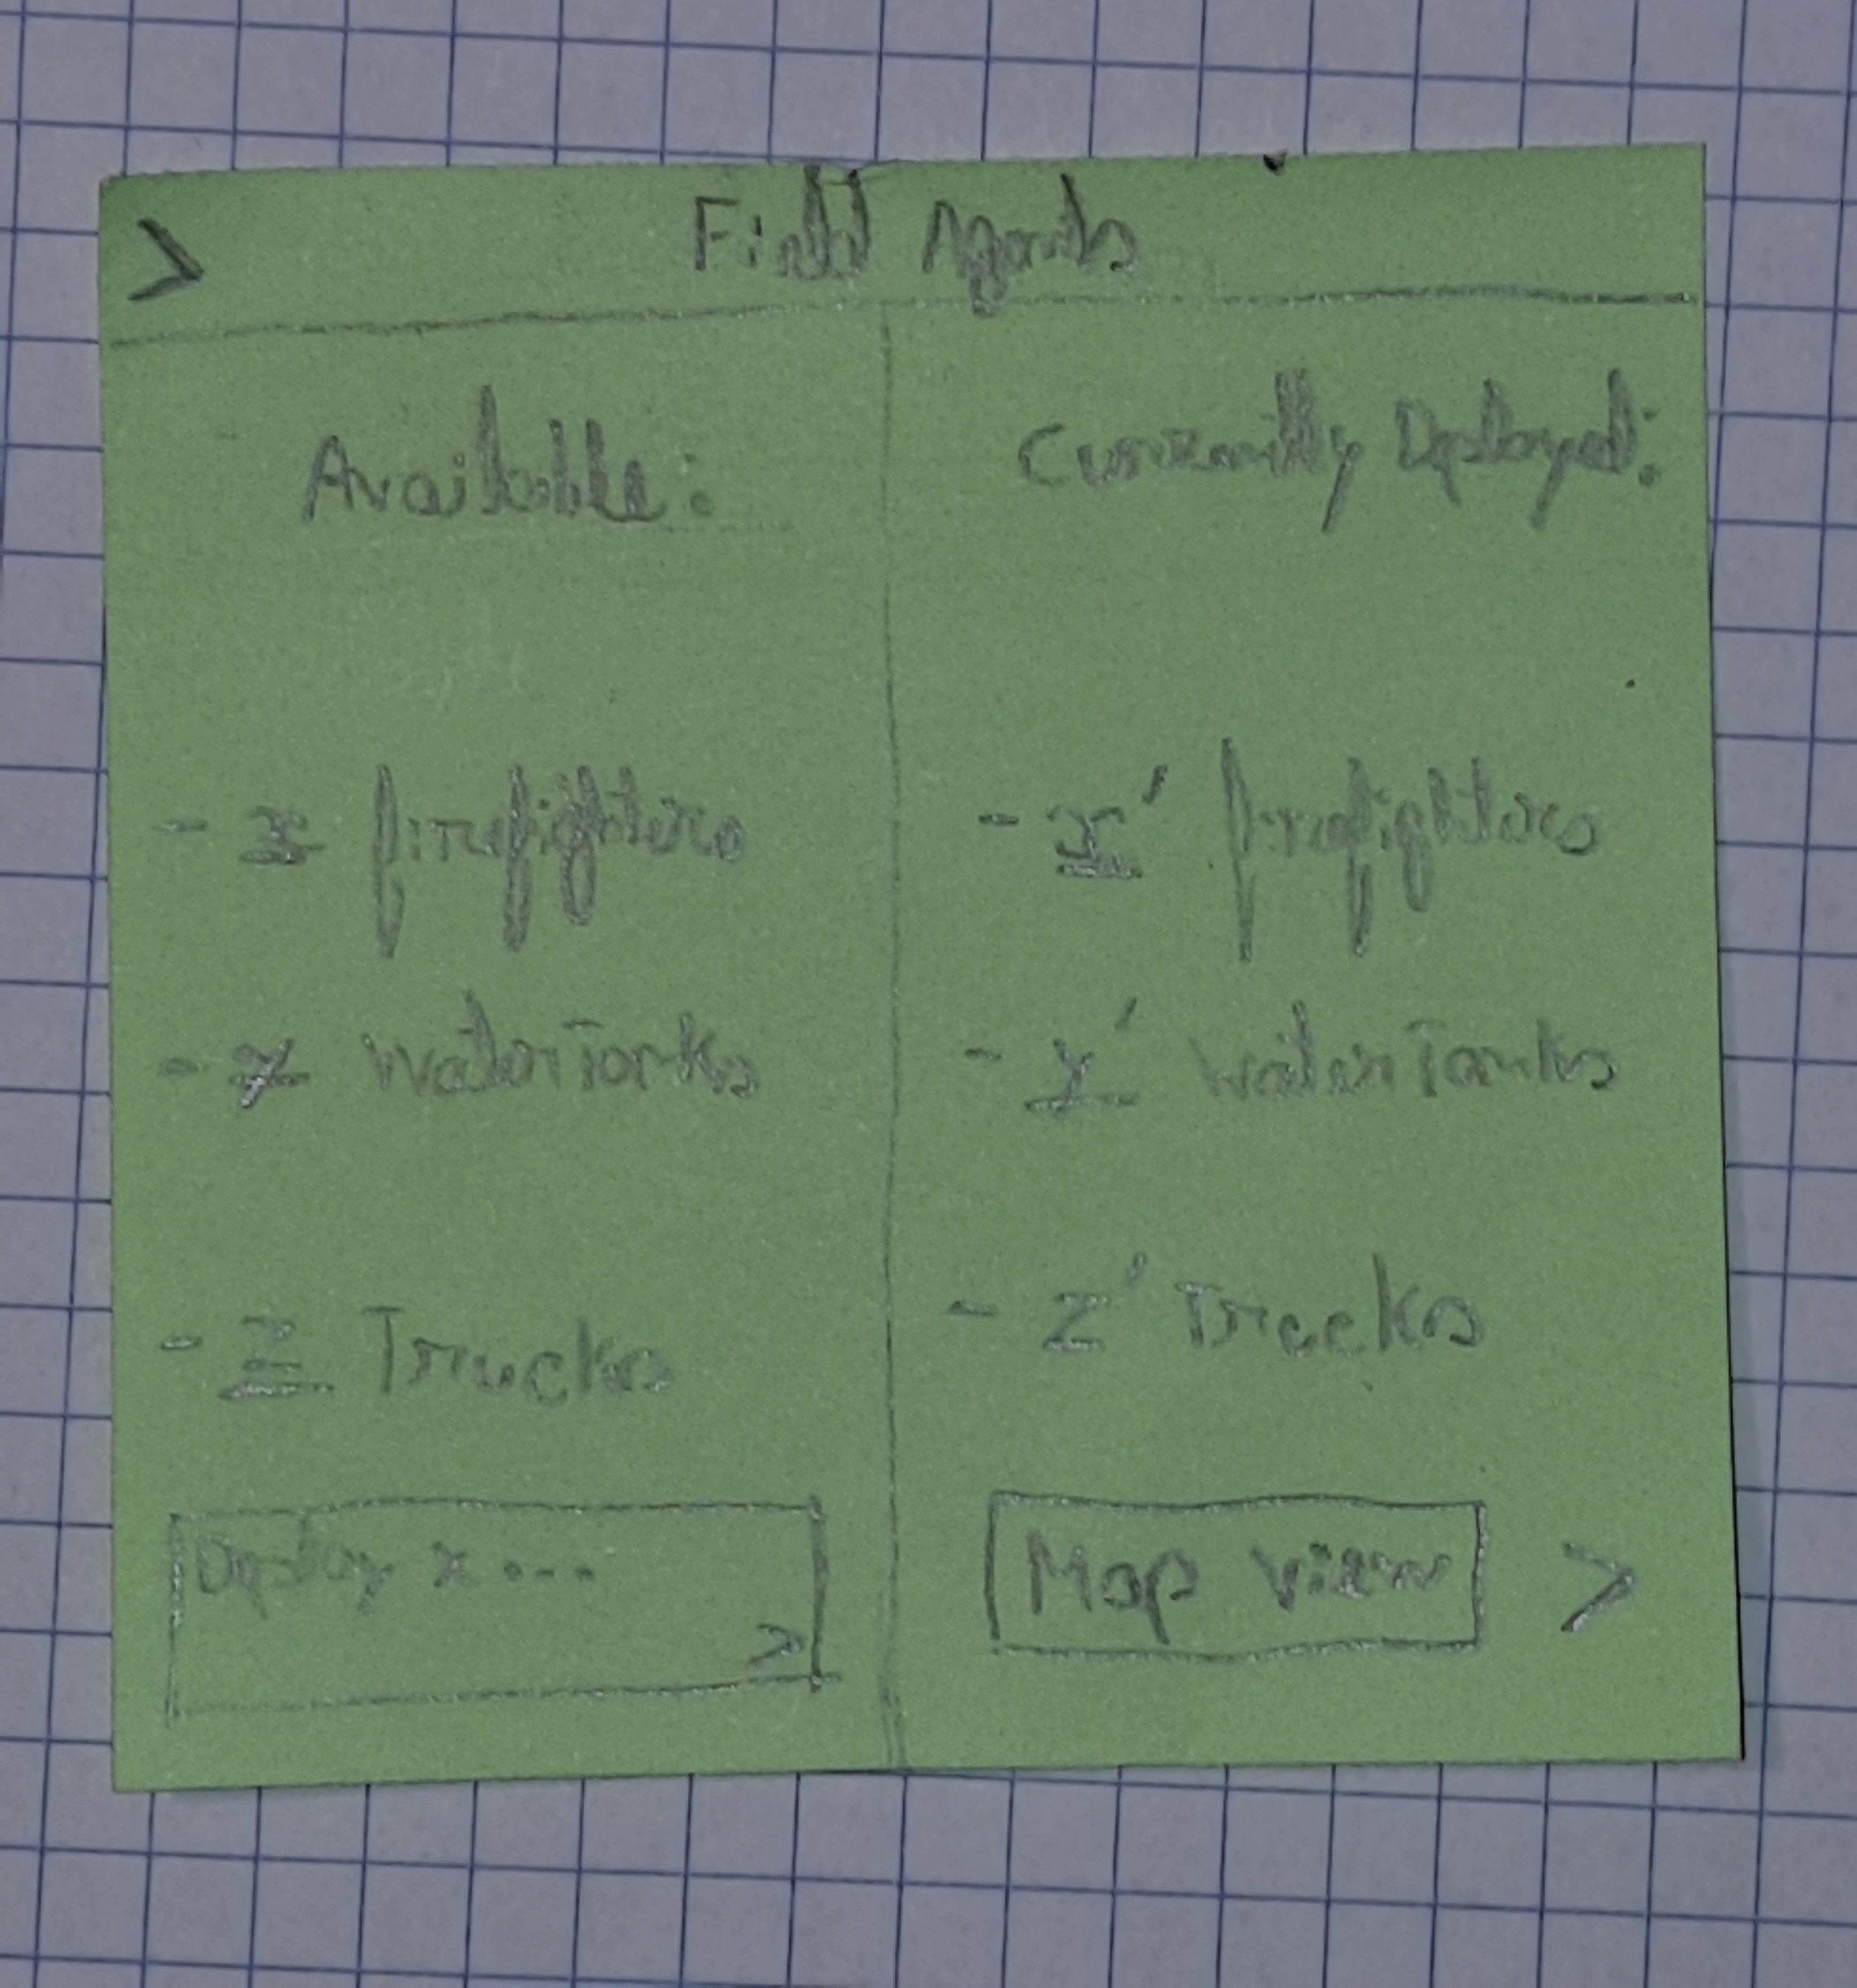
\includegraphics[width=.45\textwidth]{sketches/Resources_8(2).jpg}
            }% 
            \subfloat[Sketch 8c]{
                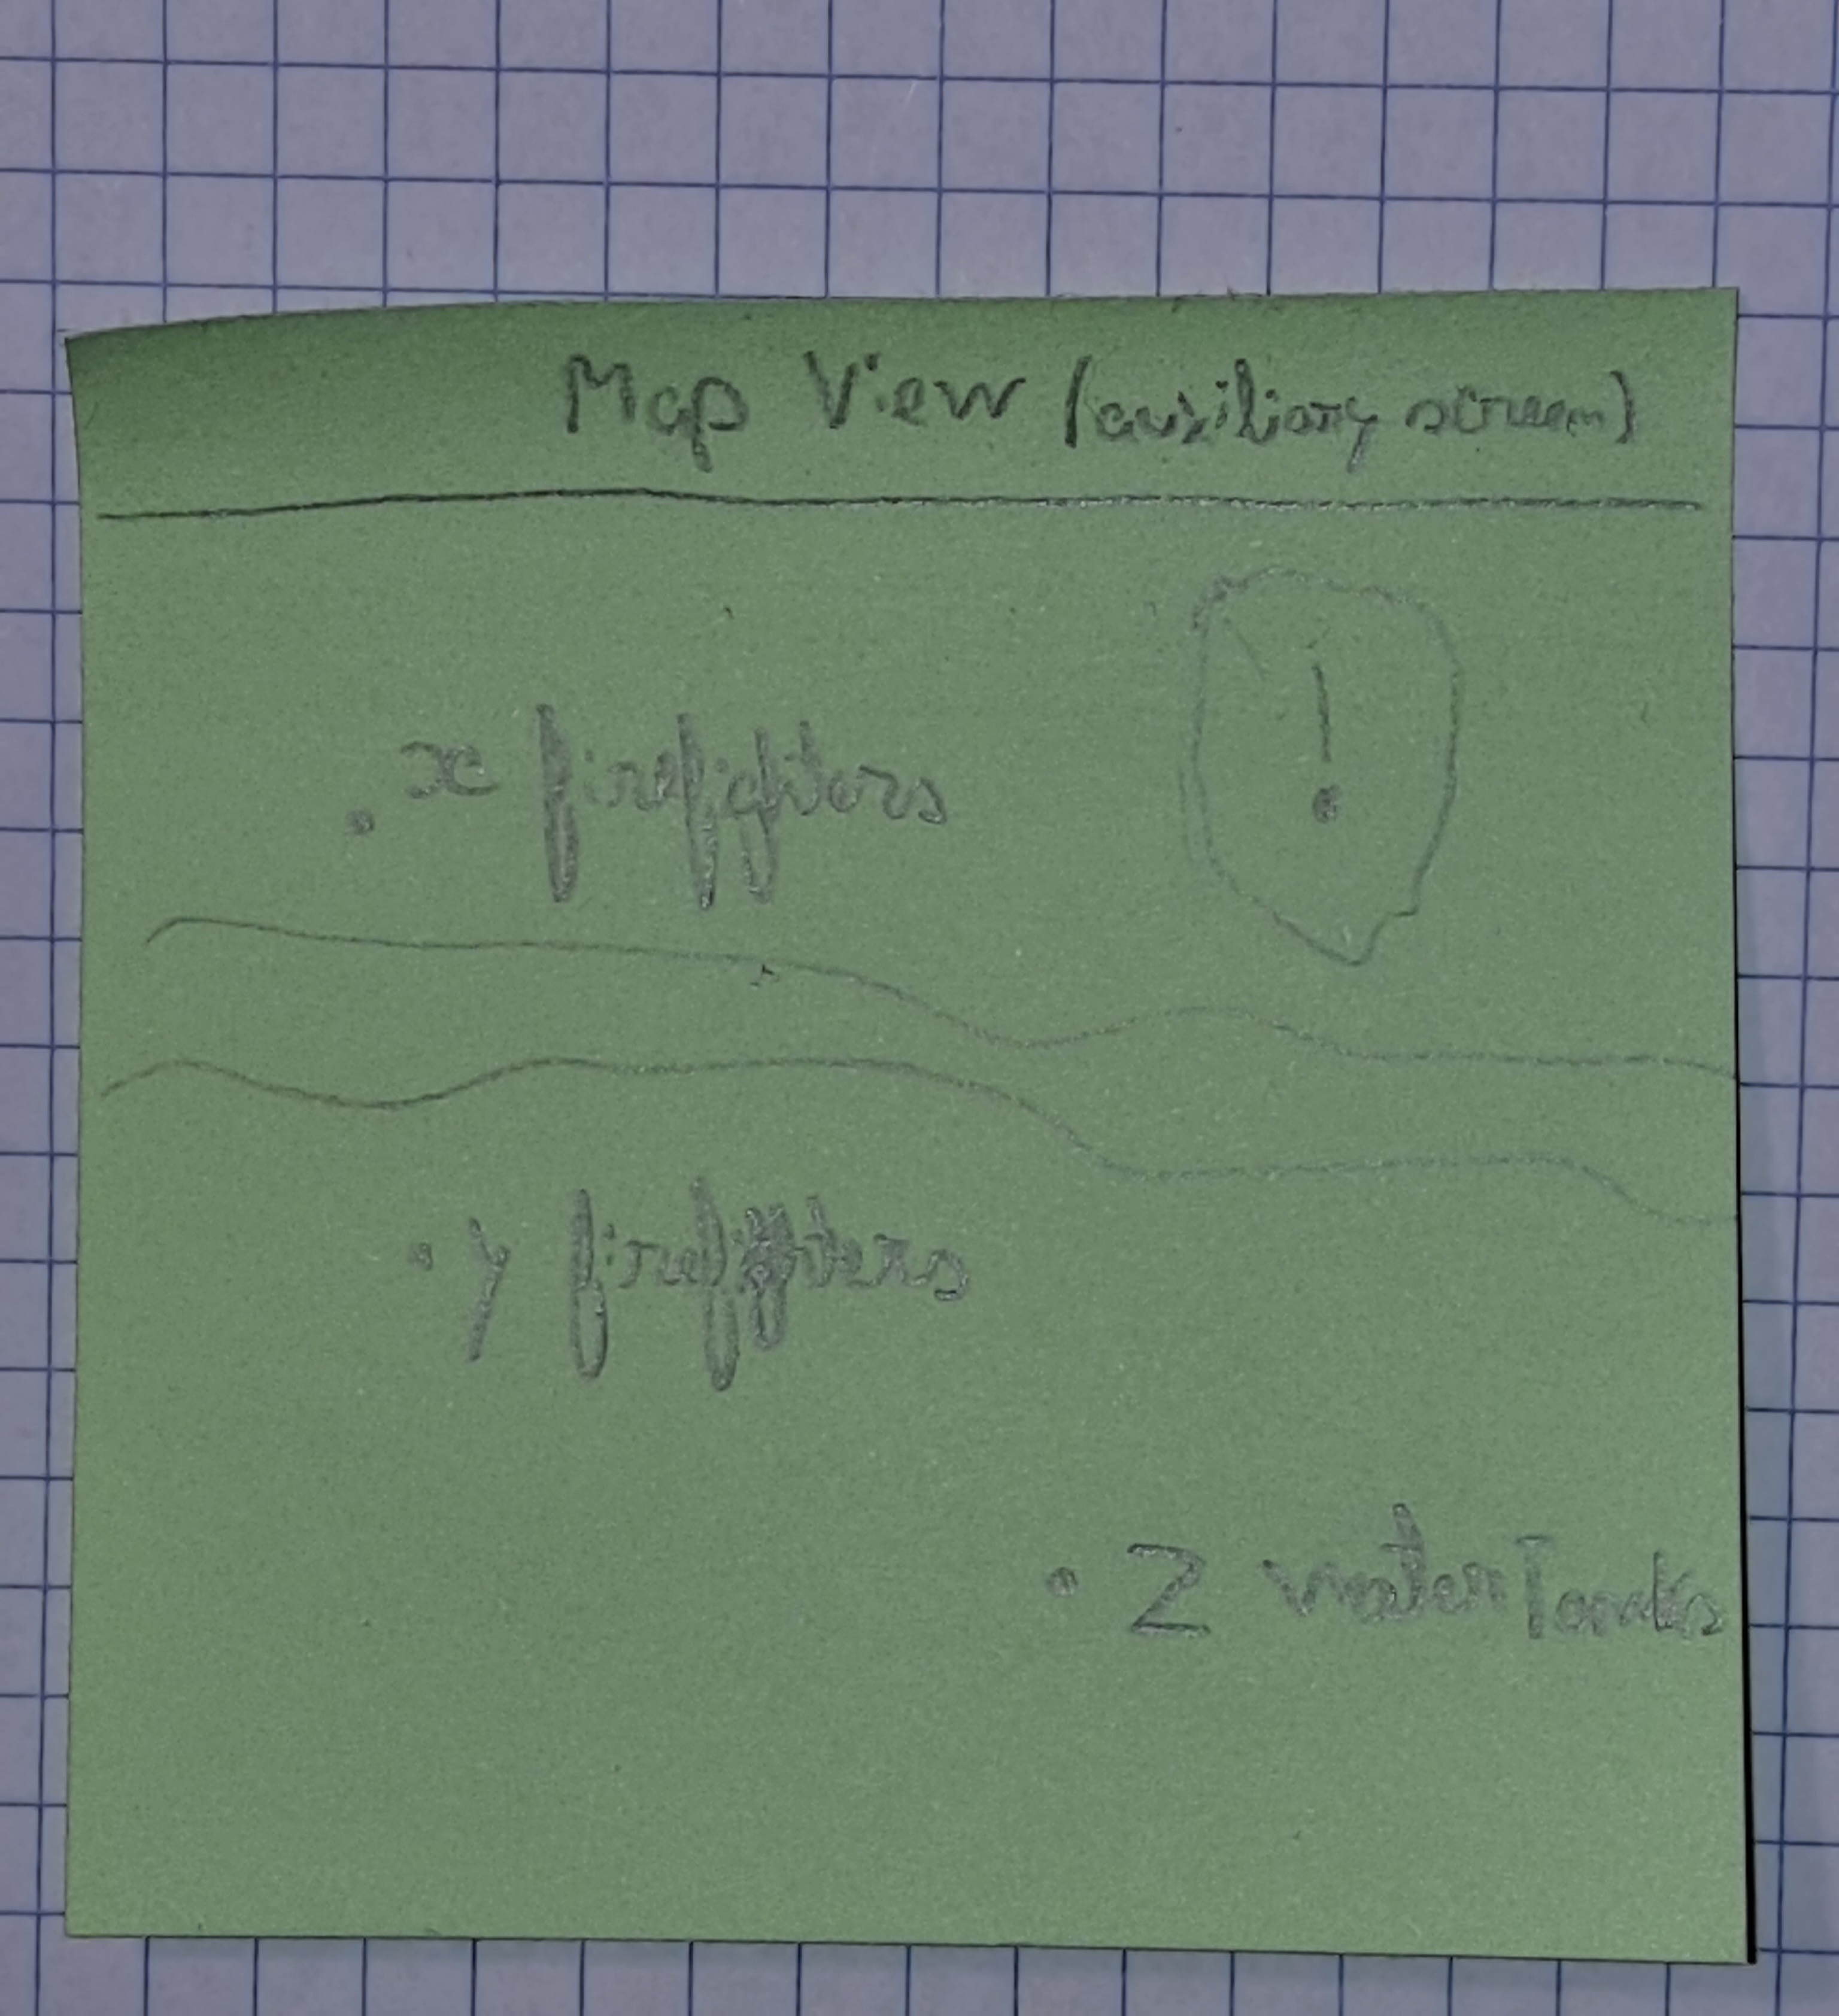
\includegraphics[width=.4\textwidth]{sketches/Resources_8(3).jpg}
            }%%
            }
        \caption{Resources Panel Sketches}
        \end{figure}
\end{itemize}
\section{Metrics Used for Evaluation}
In order to evaluate the preliminary sketches that were produced, it was
collectively determined that each sketch would be assessed according to four
distinct criteria. \par 
The criteria were defined as follows:
\begin{enumerate}
    \item Functionality;
    \item Intuitiveness or clarity;
    \item Organization;
    \item Attractiveness/Design. 
\end{enumerate} \par 
Once all members of the group had evaluated the sketches, we proceeded to
construct a matrix based on the above-mentioned four criteria. In this manner, a
ranking was established, thereby facilitating discussion and progression in the
process with regard to the most promising sketches.
\section{Evaluation and Results}
This section presents the evaluation grids for the initial sketches. \par
\textbf{Cameras Panel}
\begin{itemize}
    \item Functionality: 
\begin{table}[H]
\centerline{%
\begin{tabular}{l*{9}{c}}
& Sketch 1 & Sketch 2 & Sketch 3 & Sketch 4 
& Sketch 5 & Sketch 6 & Sketch 7 & Sketch 8 & Sketch 9 \\
\hline 
Helena & 2 & 4 & 2 & 4 & 4 & 4 & 4 & 4 & 4 \\
Tomás & 3 & 3 & 3 & 4 & 4 & 4 & 4 & 3 & 3 \\ 
Rui & 2 & 3 & 2 & 3 & 3 & 2 & 3 & 3 & 3 \\ 
Sérgio & 2 & 3 & 2 & 3 & 3 & 2 & 3 & 3 & 3 \\ 
\hline
Total & 10 & 14 & 9 & 14 & 14 & 14 & 15 & 14 & 13 \\
\end{tabular}%
}
\end{table}
\item Intuitiveness: 
\begin{table}[H]
    \centerline{%
\begin{tabular}{l*{9}{c}}
    & Sketch 1 & Sketch 2 & Sketch 3 & Sketch 4 
    & Sketch 5 & Sketch 6 & Sketch 7 & Sketch 8 & Sketch 9 \\
    \hline 
    Helena & 3 & 4 & 2 & 4 & 3 & 3 & 4 & 4 & 4 \\
    Tomás & 2 & 3 & 2 & 4 & 3 & 3 & 4 & 3 & 3 \\ 
    Rui & 4 & 4 & 2 & 2 & 3 & 3 & 4 & 4 & 3 \\ 
    Sérgio & 2 & 3 & 2 & 4 & 3 & 2 & 2 & 3 & 3 \\ 
    \hline
    Total & 11 & 14 & 8 & 14 & 12 & 11 & 14 & 14 & 13 \\
\end{tabular}%
    }
\end{table}
\item Organization:
\begin{table}[H]
    \centerline{%
    \begin{tabular}{l*{9}{c}}
        & Sketch 1 & Sketch 2 & Sketch 3 & Sketch 4 
        & Sketch 5 & Sketch 6 & Sketch 7 & Sketch 8 & Sketch 9 \\
        \hline 
        Helena & 3 & 4 & 3 & 3 & 4 & 4 & 4 & 4 & 4 \\
        Tomás & 2 & 3 & 2 & 4 & 3 & 3 & 4 & 3 & 3 \\ 
        Rui & 4 & 4 & 2 & 2 & 3 & 3 & 4 & 4 & 3 \\ 
        Sérgio & 2 & 4 & 2 & 4 & 3 & 4 & 4 & 4 & 3 \\ 
        \hline
        Total & 11 & 15 & 9 & 13 & 13 & 14 & 16 & 15 & 13 \\
    \end{tabular}%
    }
\end{table}
\item Attractiveness: 
\begin{table}[H]
    \centerline{%
    \begin{tabular}{l*{9}{c}}
        & Sketch 1 & Sketch 2 & Sketch 3 & Sketch 4 
        & Sketch 5 & Sketch 6 & Sketch 7 & Sketch 8 & Sketch 9 \\
        \hline 
        Helena & 2 & 4 & 1 & 3 & 4 & 3 & 3 & 3 & 4 \\
        Tomás & 2 & 3 & 1 & 3 & 4 & 3 & 4 & 3 & 3 \\ 
        Rui & 4 & 4 & 1 & 2 & 4 & 3 & 3 & 4 & 3 \\ 
        Sérgio & 2 & 3 & 1 & 4 & 3 & 2 & 3 & 3 & 3 \\ 
        \hline
        Total & 10 & 14 & 4 & 12 & 15 & 11 & 13 & 13 & 13 \\
    \end{tabular}%
    }
\end{table}
\item Final Results:
\begin{table}[H]
    \centerline{%
    \begin{tabular}{l*{9}{c}}
        & Sketch 1 & Sketch 2 & Sketch 3 & Sketch 4 
        & Sketch 5 & Sketch 6 & Sketch 7 & Sketch 8 & Sketch 9 \\
        \hline 
        Functionality & 10 & 14 & 9 & 14 & 14 & 14 & 15 & 14 & 13 \\
        Intuitiveness & 11 & 14 & 8 & 14 & 12 & 11 & 14 & 14 & 13 \\ 
        Organization & 11 & 15 & 9 & 13 & 13 & 14 & 16 & 15 & 13 \\ 
        Attractiveness & 10 & 14 & 4 & 12 & 15 & 11 & 13 & 13 & 13 \\ 
        \hline
        Total & 42 & 57 & 30 & 53 & 54 & 50 & 58 & 56 & 52 \\
    \end{tabular}% 
    }
\end{table}
\end{itemize} \par
Here, we come to the conlusion that the top 3 sketeches are
sketches 7, 2 and 8. \\\\
\textbf{Log Panel}
\begin{itemize}
    \item Functionality: 
\begin{table}[H]
\centerline{%
\begin{tabular}{l*{5}{c}}
    & Sketch 1 & Sketch 2 & Sketch 3 & Sketch 4 & Sketch 5 \\
    \hline 
    Helena & 4 & 4 & 4 & 4 & 4 \\
    Tomás & 4 & 3 & 3 & 3 & 3 \\ 
    Rui & 4 & 4 & 3 & 4 & 3 \\ 
    Sérgio & 2 & 3 & 3 & 3 & 3 \\ 
    \hline
    Total & 14 & 14 & 13 & 14 & 13 \\
\end{tabular}%
}
\end{table}
    \item Intuitiveness:
    \begin{table}[H]
        \centerline{%
        \begin{tabular}{l*{5}{c}}
            & Sketch 1 & Sketch 2 & Sketch 3 & Sketch 4 & Sketch 5 \\
            \hline 
            Helena & 4 & 4 & 4 & 4 & 4 \\
            Tomás & 4 & 3 & 3 & 3 & 3 \\ 
            Rui & 4 & 4 & 3 & 4 & 3 \\ 
            Sérgio & 2 & 3 & 3 & 3 & 3 \\ 
            \hline
            Total & 14 & 14 & 13 & 14 & 13 \\
        \end{tabular}% 
        }
        \end{table}
\item Organization:
 \begin{table}[H]
    \centerline{%
    \begin{tabular}{l*{5}{c}}
        & Sketch 1 & Sketch 2 & Sketch 3 & Sketch 4 & Sketch 5 \\
        \hline 
        Helena & 4 & 4 & 3 & 3 & 4 \\
        Tomás & 3 & 4 & 4 & 3 & 3 \\ 
        Rui & 4 & 4 & 4 & 3 & 3 \\ 
        Sérgio & 2 & 3 & 3 & 3 & 3 \\ 
        \hline
        Total & 13 & 15 & 14 & 12 & 13 \\
    \end{tabular}%
    }
    \end{table}
\item Attractiveness:
\begin{table}[H]
    \centerline{%
    \begin{tabular}{l*{5}{c}}
        & Sketch 1 & Sketch 2 & Sketch 3 & Sketch 4 & Sketch 5 \\
        \hline 
        Helena & 4 & 4 & 4 & 4 & 4 \\
        Tomás & 4 & 3 & 3 & 3 & 3 \\ 
        Rui & 4 & 4 & 3 & 4 & 3 \\ 
        Sérgio & 2 & 3 & 3 & 3 & 3 \\ 
        \hline
        Total & 14 & 14 & 13 & 14 & 13 \\
    \end{tabular}% 
    }
    \end{table}
\item Final Results:
\begin{table}[H]
    \centerline{%
    \begin{tabular}{l*{5}{c}}
        & Sketch 1 & Sketch 2 & Sketch 3 & Sketch 4 & Sketch 5 \\
        \hline 
        Functionality & 14 & 14 & 13 & 14 & 13 \\
        Intuitiveness & 12 & 14 & 13 & 14 & 12 \\ 
        Organization & 13 & 15 & 14 & 12 & 13 \\ 
        Attractiveness & 11 & 16 & 14 & 12 & 13 \\ 
        \hline
        Total & 50 & 59 & 54 & 52 & 51 \\
    \end{tabular}%
    }
    \end{table}
\end{itemize} \par 
Here, we come to the conlusion that the top 3 sketeches are
sketches 2, 3 and 4. \\\\
\textbf{Rescources Panel}
\begin{itemize}
\item Functionality:  
\begin{table}[H]
    \centerline{%
\begin{tabular}{l*{8}{c}}
    & Sketch 1 & Sketch 2 & Sketch 3 
    & Sketch 4 & Sketch 5 & Sketch 6 & Sketch 7 
    & Sketch 8 \\
    \hline 
    Helena & 4 & 4 & 4 & 4 & 4 & 4 & 4 & 4 \\ 
    Tomás & 3 & 4 & 3 & 2 & 3 & 4 & 4 & 3 \\ 
    Rui & 3 & 3 & 3 & 4 & 4 & 4 & 4 & 3 \\ 
    Sérgio & 2 & 3 & 3 & 3 & 3 & 3 & 3 & 4 \\ 
    \hline 
    Total & 12 & 14 & 13 & 13 & 14 & 15 & 15 & 14 \\
\end{tabular}% 
    }
\end{table}
\item Intuitiveness: 
\begin{table}[H]
    \centerline{%
    \begin{tabular}{l*{8}{c}}
        & Sketch 1 & Sketch 2 & Sketch 3 
        & Sketch 4 & Sketch 5 & Sketch 6 & Sketch 7 
        & Sketch 8 \\
        \hline 
        Helena & 4 & 4 & 4 & 4 & 4 & 4 & 4 & 4 \\ 
        Tomás & 3 & 4 & 2 & 3 & 3 & 4 & 4 & 2 \\ 
        Rui & 3 & 4 & 2 & 3 & 2 & 4 & 4 & 4 \\ 
        Sérgio & 2 & 3 & 3 & 3 & 2 & 3 & 3 & 4 \\ 
        \hline 
        Total & 12 & 15 & 11 & 13 & 11 & 15 & 15 & 14 \\
    \end{tabular}%
    }
    \end{table}
\item Organization: 
\begin{table}[H]
    \centerline{%
    \begin{tabular}{l*{8}{c}}
        & Sketch 1 & Sketch 2 & Sketch 3 
        & Sketch 4 & Sketch 5 & Sketch 6 & Sketch 7 
        & Sketch 8 \\
        \hline 
        Helena & 4 & 4 & 4 & 4 & 4 & 4 & 4 & 4 \\ 
        Tomás & 3 & 4 & 3 & 3 & 4 & 4 & 4 & 3 \\ 
        Rui & 4 & 4 & 4 & 2 & 4 & 4 & 4 & 3 \\ 
        Sérgio & 2 & 3 & 3 & 3 & 2 & 3 & 4 & 3 \\ 
        \hline 
        Total & 13 & 15 & 14 & 12 & 15 & 15 & 16 & 15 \\
    \end{tabular}%
    }
    \end{table}
\item Attractiveness:
    \begin{table}[H]
        \centerline{%
        \begin{tabular}{l*{8}{c}}
            & Sketch 1 & Sketch 2 & Sketch 3 
            & Sketch 4 & Sketch 5 & Sketch 6 & Sketch 7 
            & Sketch 8 \\
            \hline 
            Helena & 4 & 4 & 3 & 4 & 3 & 4 & 4 & 3 \\ 
            Tomás & 3 & 4 & 2 & 2 & 3 & 4 & 4 & 2 \\ 
            Rui & 3 & 4 & 2 & 2 & 3 & 4 & 4 & 2 \\ 
            Sérgio & 2 & 3 & 3 & 2 & 3 & 3 & 3 & 3 \\ 
            \hline 
            Total & 12 & 15 & 10 & 10 & 12 & 15 & 15 & 10 \\
        \end{tabular}%
        }
        \end{table}
\item Final Results: 
\begin{table}[H]
    \centerline{%
    \begin{tabular}{l*{8}{c}}
        & Sketch 1 & Sketch 2 & Sketch 3 
        & Sketch 4 & Sketch 5 & Sketch 6 & Sketch 7 
        & Sketch 8 \\
        \hline 
        Functionality & 12 & 14 & 13 & 13 & 14 & 15 & 15 & 14 \\ 
        Intuitiveness & 12 & 15 & 11 & 13 & 11 & 15 & 15 & 14 \\ 
        Organization & 13 & 15 & 14 & 12 & 15 & 15 & 16 & 13 \\ 
        Attractiveness & 12 & 15 & 10 & 10 & 12 & 15 & 15 & 10 \\ 
        \hline 
        Total & 49 & 59 & 48 & 48 & 52 & 60 & 61 & 51 \\
    \end{tabular}%
    }
    \end{table}
\end{itemize} \par
Here, we come to the conlusion that the top 3 sketeches are
sketches 2, 6 and 7. \\\\
\textbf{Situation Panel}
\begin{itemize}
    \item Single:
    \begin{itemize}
        \item Functionality:
        \begin{table}[H]
            \caption{Functionality Results Table}
            \centerline{%
            \begin{tabular}{l*{9}{c}}
            & Sketch 1 & Sketch 2 & Sketch 3 & Sketch 4 
            & Sketch 5 & Sketch 6 & Sketch 7 & Sketch 8 & Sketch 9 \\
            \hline 
            Helena & 2 & 3 & 3 & 3 & 3 & 4 & 3 & 3 & 3 \\
            Tomás & 2 & 3 & 4 & 4 & 4 & 4 & 3 & 3 & 3 \\ 
            Rui & 2 & 3 & 3 & 4 & 4 & 4 & 3 & 3 & 2 \\ 
            Sérgio & 2 & 3 & 4 & 3 & 4 & 3 & 4 & 3 & 3 \\ 
            \hline
            Total & 8 & 12 & 14 & 14 & 15 & 15 & 13 & 12 & 10 \\
            \end{tabular}%
            }
            \end{table}
            \item Intuitiveness: 
            \begin{table}[H]
                \caption{Functionality Results Table}
                \centerline{%
                \begin{tabular}{l*{9}{c}}
                & Sketch 1 & Sketch 2 & Sketch 3 & Sketch 4 
                & Sketch 5 & Sketch 6 & Sketch 7 & Sketch 8 & Sketch 9 \\
                \hline 
                Helena & 2 & 2 & 4 & 3 & 4 & 4 & 3 & 3 & 2 \\
                Tomás & 2 & 2 & 3 & 3 & 4 & 4 & 2 & 3 & 2 \\ 
                Rui & 2 & 2 & 3 & 4 & 4 & 4 & 2 & 3 & 2 \\ 
                Sérgio & 3 & 2 & 4 & 2 & 4 & 4 & 4 & 2 & 4 \\ 
                \hline
                Total & 9 & 8 & 14 & 12 & 16 & 16 & 11 & 11 & 10 \\
                \end{tabular}%
                }
            \end{table}
            \item Organization: 
            \begin{table}[H]
               % \caption{Functionality Results Table}
               \centerline{%
                \begin{tabular}{l*{9}{c}}
                & Sketch 1 & Sketch 2 & Sketch 3 & Sketch 4 
                & Sketch 5 & Sketch 6 & Sketch 7 & Sketch 8 & Sketch 9 \\
                \hline 
                Helena & 1 & 2 & 3 & 3 & 4 & 4 & 4 & 3 & 3 \\
                Tomás & 1 & 2 & 4 & 3 & 4 & 4 & 3 & 3 & 2 \\ 
                Rui & 1 & 2 & 2 & 3 & 4 & 4 & 3 & 3 & 3 \\ 
                Sérgio & 2 & 2 & 4 & 3 & 4 & 4 & 4 & 2 & 3 \\ 
                \hline
                Total & 5 & 8 & 13 & 12 & 16 & 16 & 14 & 11 & 11 \\
                \end{tabular}%
               }
                \end{table}
            \item Attractiveness:
            \begin{table}[H]
                %\caption{Functionality Results Table}
                \centerline{%
                \begin{tabular}{l*{9}{c}}
                & Sketch 1 & Sketch 2 & Sketch 3 & Sketch 4 
                & Sketch 5 & Sketch 6 & Sketch 7 & Sketch 8 & Sketch 9 \\
                \hline 
                Helena & 1 & 3 & 3 & 3 & 3 & 4 & 4 & 4 & 4 \\
                Tomás & 1 & 2 & 2 & 3 & 4 & 4 & 3 & 3 & 2 \\ 
                Rui & 1 & 2 & 2 & 2 & 3 & 4 & 4 & 4 & 3 \\ 
                Sérgio & 1 & 3 & 3 & 3 & 2 & 3 & 3 & 4 & 2 \\ 
                \hline
                Total & 4 & 10 & 10 & 11 & 12 & 15 & 14 & 15 & 12 \\
                \end{tabular}%
                }
                \end{table}
    \end{itemize}
\begin{table}[H]
    \centerline{%
    \begin{tabular}{l*{9}{c}}
        & Sketch 1 & Sketch 2 & Sketch 3 & Sketch 4 
        & Sketch 5 & Sketch 6 & Sketch 7 & Sketch 8 & Sketch 9 \\
        \hline 
        Functionality & 8 & 12 & 14 & 14 & 15 & 15 & 13 & 12 & 10 \\
        Intuitiveness & 9 & 8 & 14 & 12 & 16 & 16 & 11 & 11 & 10 \\ 
        Organization & 5 & 8 & 13 & 12 & 16 & 16 & 14 & 11 & 11 \\ 
        Attractiveness & 4 & 10 & 10 & 11 & 12 & 15 & 14 & 15 & 12 \\ 
        \hline
        Total & 26 & 38 & 51 & 49 & 59 & 62 & 52 & 49 & 43 \\
    \end{tabular}%
    }
\end{table} \par 
Here, we come to the conlusion that the top 3 sketeches are
sketches 5, 6 and 7. \\\\
    \item Multiple:
    \begin{table}[H]
        \centerline{%
        \begin{tabular}{l*{6}{c}}
            & Sketch 1 & Sketch 2 & Sketch 3 & Sketch 4 & Sketch 5 & Sketch 6 \\
            \hline 
            Helena & 4 & 4 & 4 & 4 & 4 & 4 \\
            Tomás & 2 & 3 & 3 & 3 & 3 & 4 \\ 
            Rui & 2 & 3 & 4 & 4 & 3 & 4 \\ 
            Sérgio & 4 & 3 & 3 & 3 & 2 & 3 \\ 
            \hline
            Total & 12 & 13 & 14 & 14 & 12 & 15 \\
        \end{tabular}%
        }
        \end{table}
    \item Intuitiveness:
    \begin{table}[H]
        \centerline{%
        \begin{tabular}{l*{6}{c}}
            & Sketch 1 & Sketch 2 & Sketch 3 & Sketch 4 & Sketch 5 & Sketch 6 \\
            \hline 
            Helena & 4 & 4 & 4 & 3 & 3 & 4 \\
            Tomás & 1 & 3 & 4 & 2 & 4 & 4 \\ 
            Rui & 2 & 2 & 4 & 4 & 3 & 4 \\ 
            Sérgio & 3 & 2 & 3 & 2 & 2 & 3 \\ 
            \hline
            Total & 10 & 11 & 15 & 11 & 12 & 15 \\
        \end{tabular}%
        }
        \end{table}
    \item Organization: 
    \begin{table}[H]
        \centerline{%
        \begin{tabular}{l*{6}{c}}
            & Sketch 1 & Sketch 2 & Sketch 3 & Sketch 4 & Sketch 5 & Sketch 6 \\
            \hline 
            Helena & 4 & 3 & 4 & 4 & 3 & 4 \\
            Tomás & 1 & 2 & 4 & 3 & 2 & 3 \\ 
            Rui & 1 & 2 & 4 & 3 & 2 & 4 \\ 
            Sérgio & 3 & 2 & 3 & 2 & 2 & 3 \\ 
            \hline
            Total & 9 & 9 & 15 & 12 & 9 & 14 \\
        \end{tabular}%
        }
        \end{table}
    \item Attractiveness:
    \begin{table}[H]
        \centerline{%
        \begin{tabular}{l*{6}{c}}
            & Sketch 1 & Sketch 2 & Sketch 3 & Sketch 4 & Sketch 5 & Sketch 6 \\
            \hline 
            Helena & 3 & 3 & 4 & 3 & 3 & 4 \\
            Tomás & 1 & 2 & 3 & 3 & 2 & 3 \\ 
            Rui & 1 & 1 & 4 & 3 & 2 & 4 \\ 
            Sérgio & 4 & 3 & 3 & 2 & 2 & 2 \\ 
            \hline
            Total & 9 & 9 & 14 & 11 & 9 & 13 \\
        \end{tabular}%
        }
        \end{table}
    \item Final Scores: 
    \begin{table}[H]
        \centerline{%
        \begin{tabular}{l*{6}{c}}
            & Sketch 1 & Sketch 2 & Sketch 3 & Sketch 4 
            & Sketch 5 & Sketch 6 \\
            \hline 
            Functionality & 12 & 13 & 14 & 14 & 12 & 15  \\
            Intuitiveness & 10 & 11 & 15 & 11 & 12 & 15  \\ 
            Organization & 9 & 9 & 15 & 12 & 9 & 14  \\ 
            Attractiveness & 9 & 9 & 14 & 11 & 9 & 13  \\ 
            \hline
            Total & 40 & 42 & 58 & 48 & 42 & 57  \\
        \end{tabular}%
        }
    \end{table}
\end{itemize} \par
Here, we come to the conlusion that the top 3 sketeches are
sketches 3, 4 and 6. 
\section{Iteration Process}
To date, only one iteration has been conducted subsequent to the preliminary sketches. These sketches were developed on the foundation of the three most popular sketches from each panel. \par
It is our opinion that this process is not yet complete. It would be advantageous to engage in a discourse concerning the features and functionalities in question, subsequent to the evaluation, with a view to producing a new sketch for each of the panels. \par
Below are the most recent sketches:
\begin{itemize}
    \item \textbf{Situation Panel:}
        \begin{itemize}
            \item Multiple: 
                \begin{figure}[H]
                    \centerline{%
                    \subfloat[Sketch 7]{
                        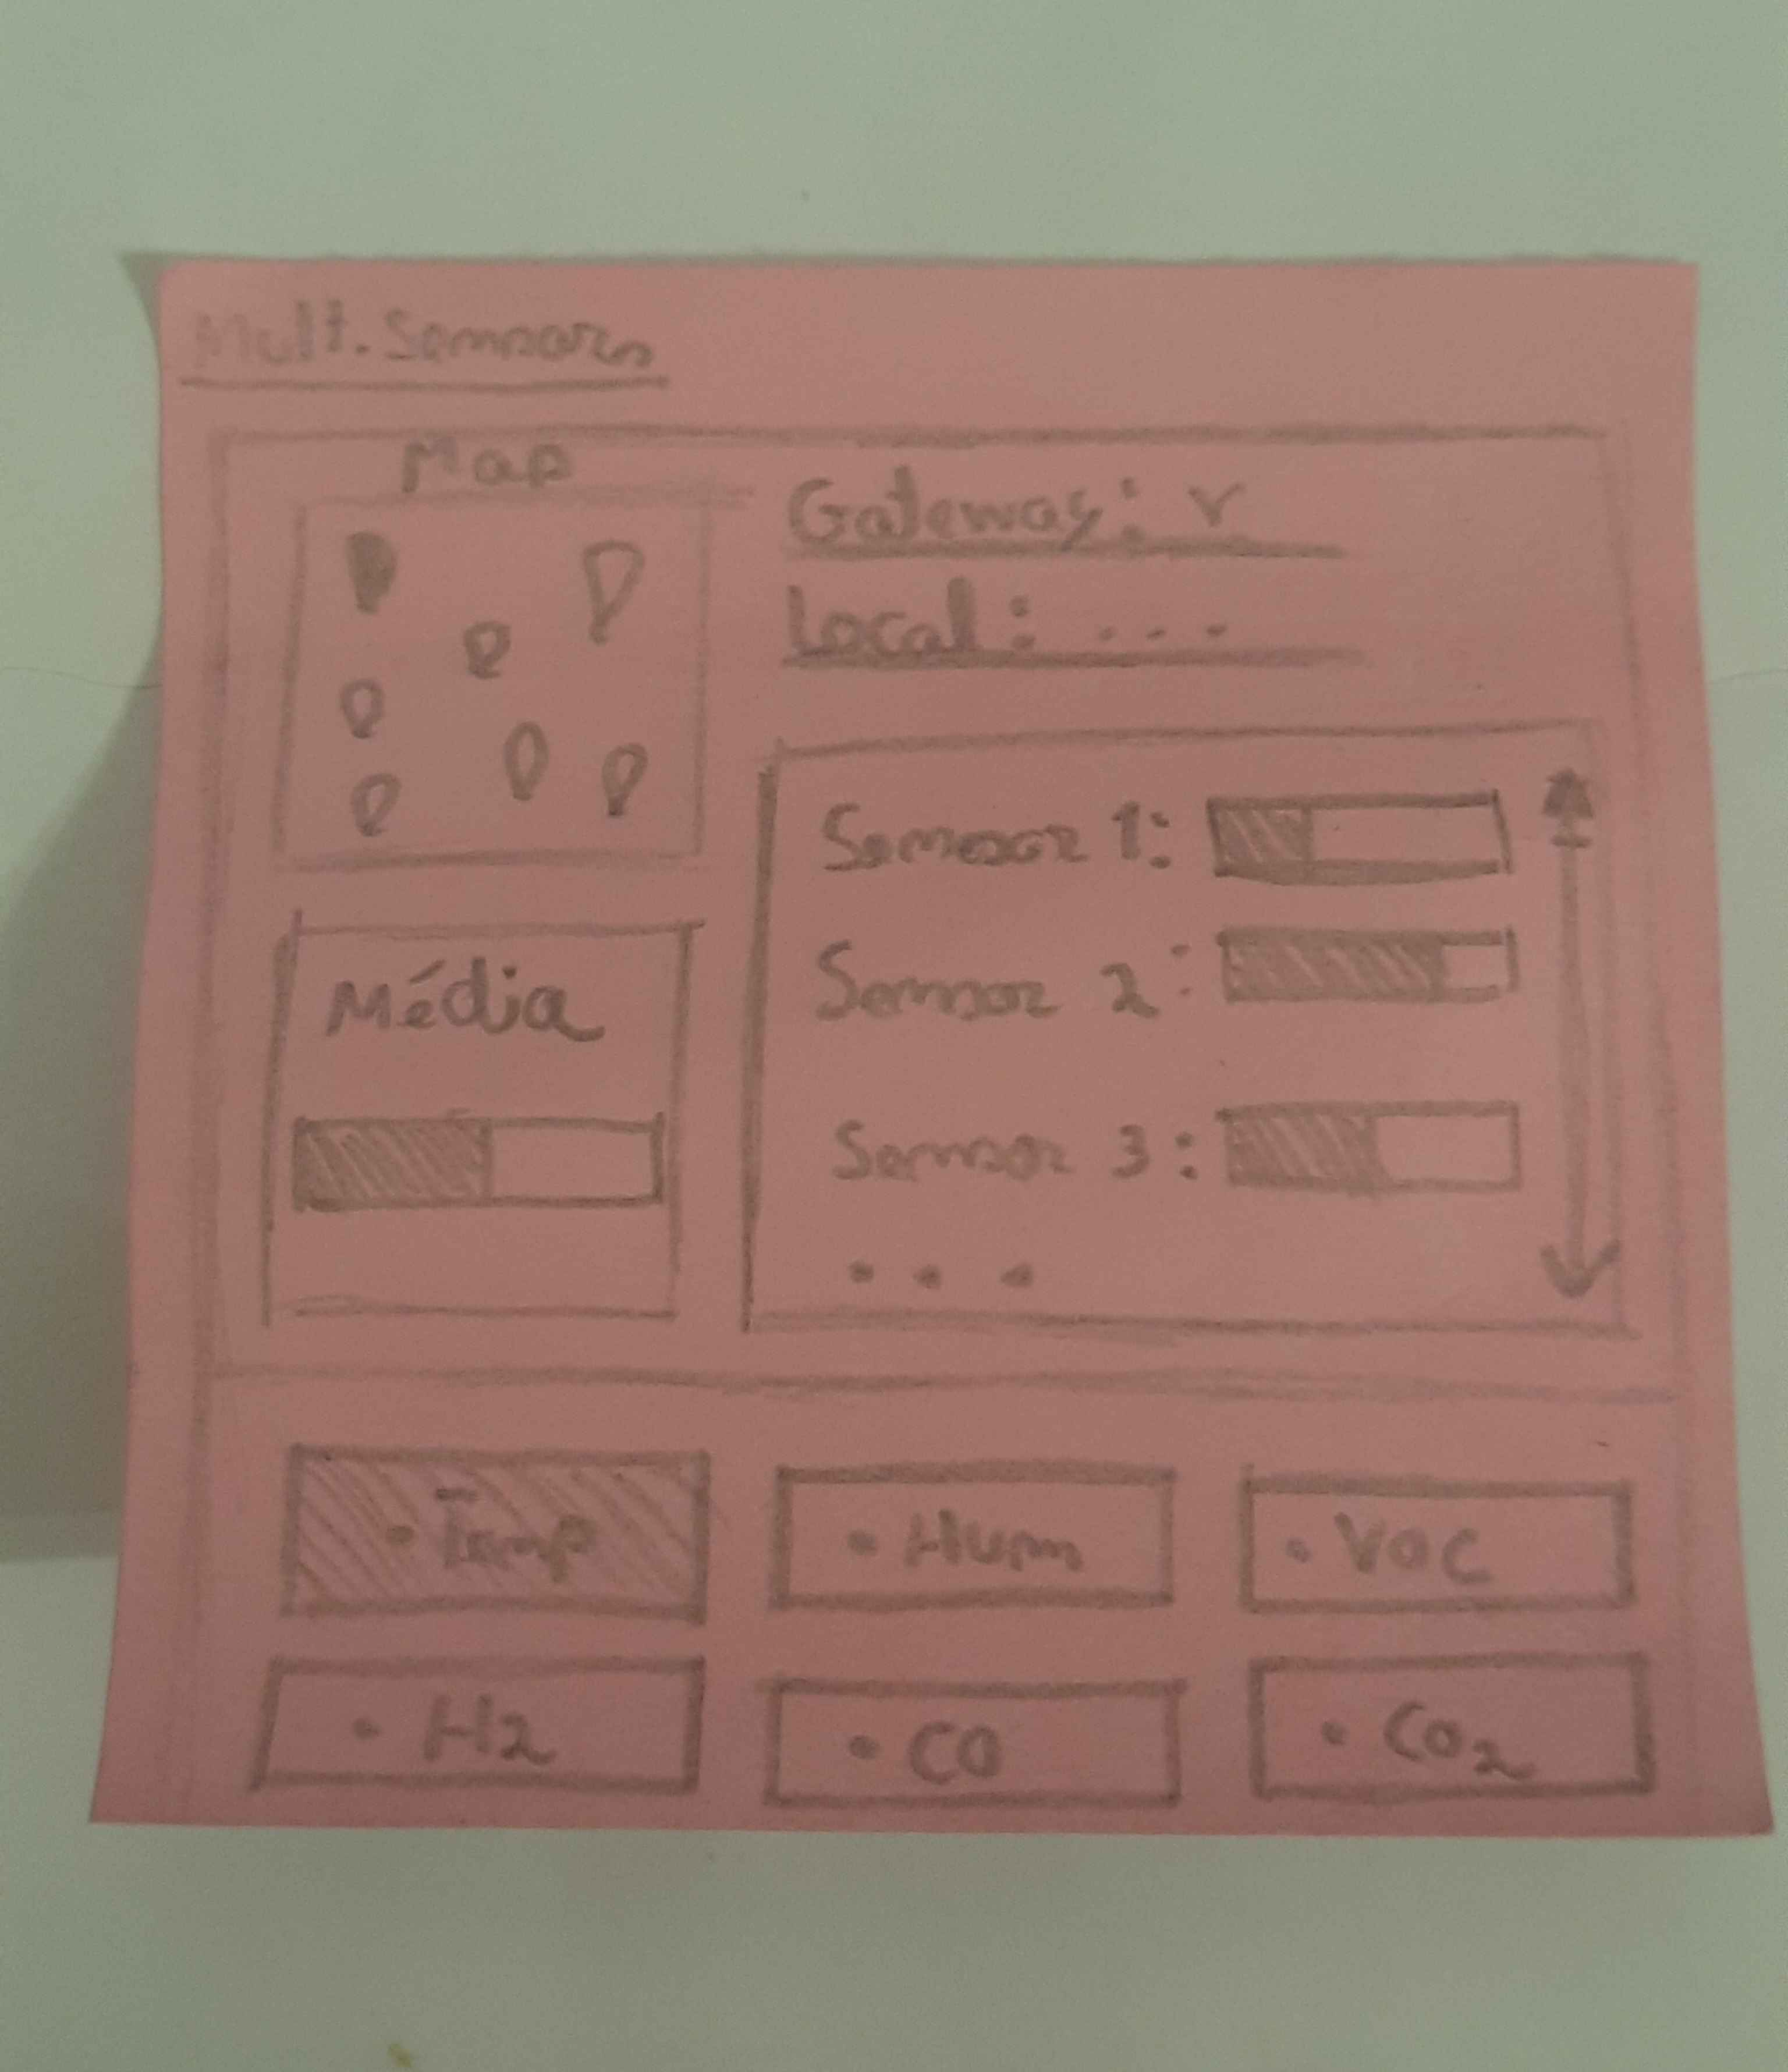
\includegraphics[width=.5\textwidth]{sketches/Situation_mult_iter(1).jpg}
                    }\hfill
                    \subfloat[Sketch 8]{
                        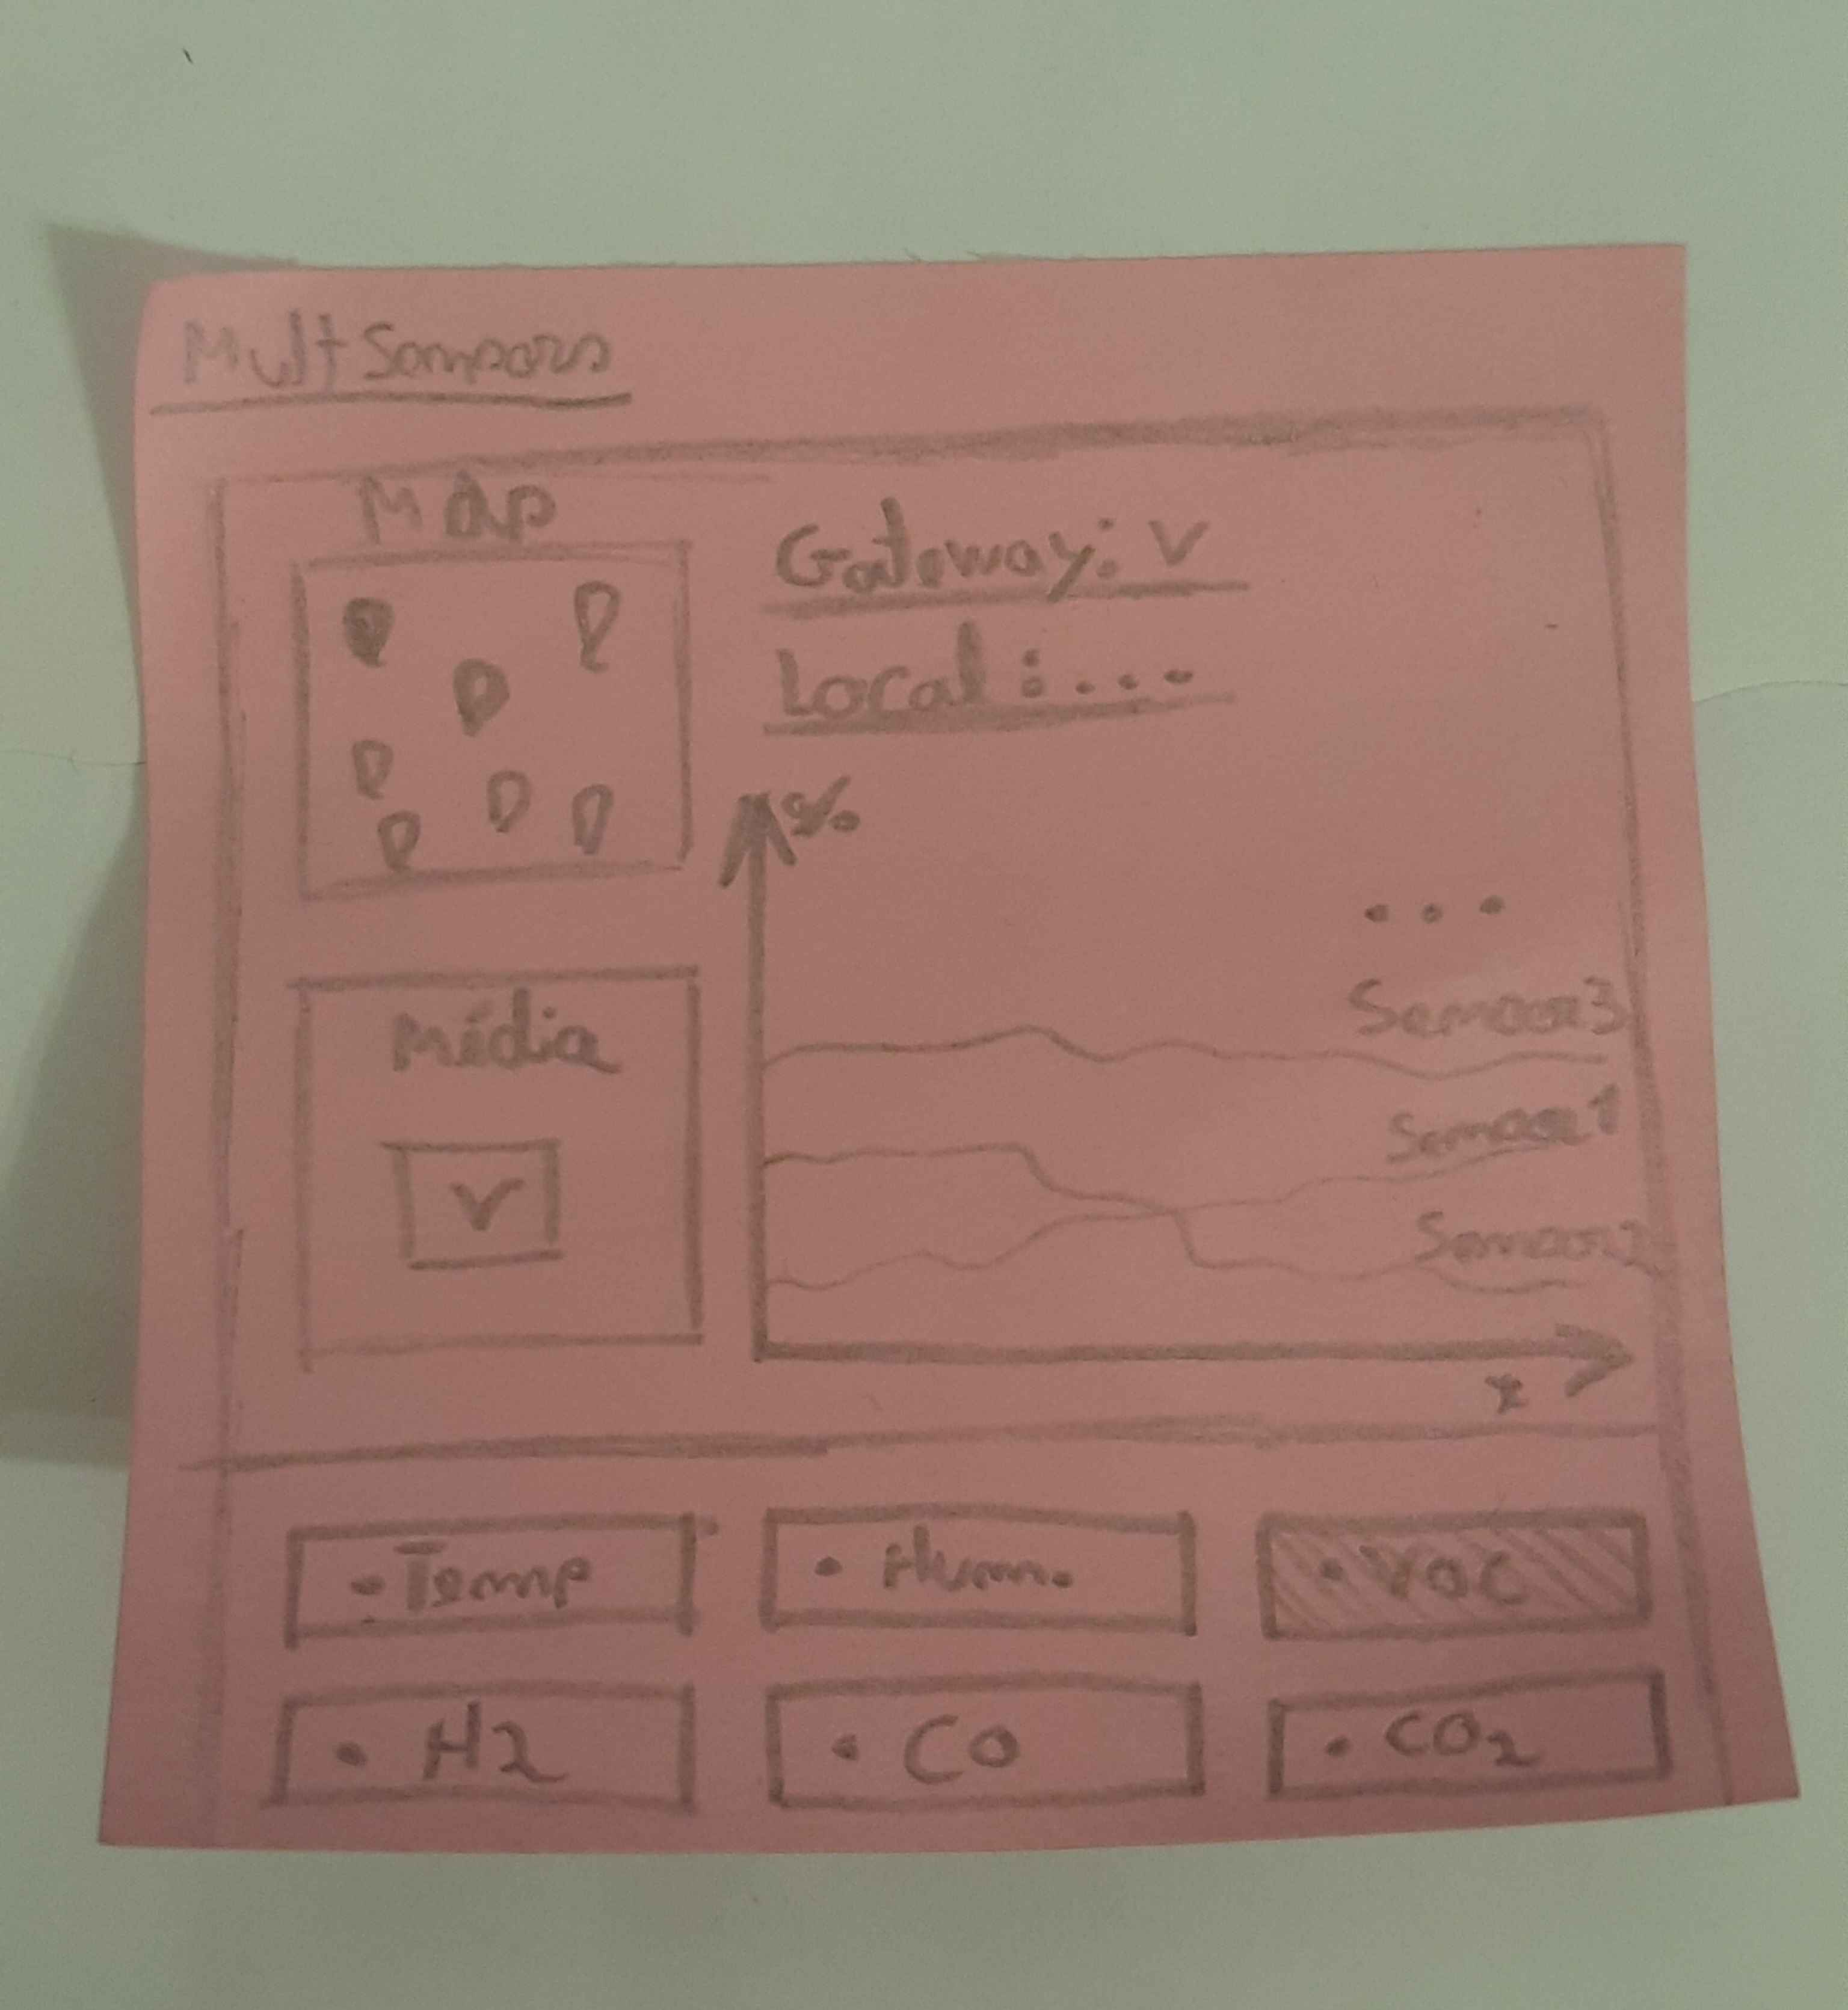
\includegraphics[width=.5\textwidth]{sketches/Situation_mult_iter(2).jpg}
                    }%
                    }
                \caption{Recent Multiple Situation Panel Sketches}
                \end{figure}
        \end{itemize}
    \item \textbf{Log Panel:}
        \begin{figure}[H]
            \centering
            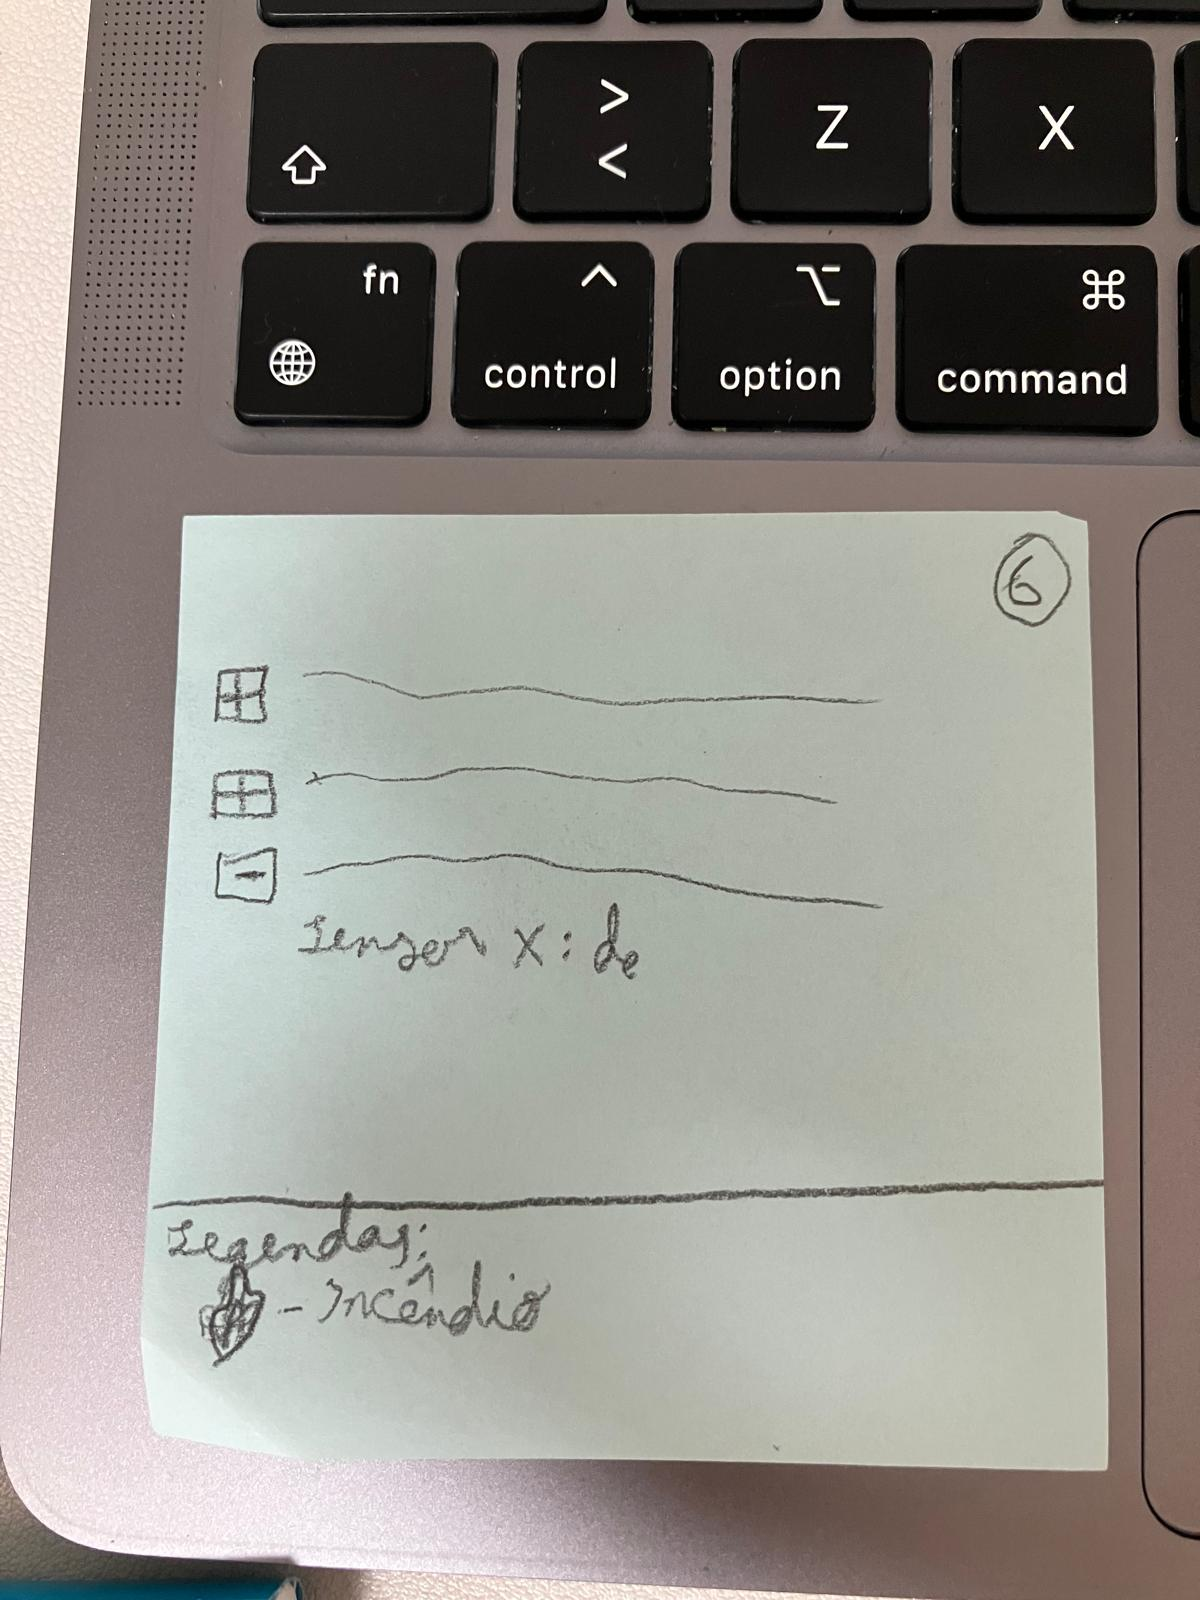
\includegraphics[width=.5\textwidth]{sketches/Log_iter.jpg}
            \caption{Recent Log Panel Sketch}
        \end{figure}
    \item \textbf{Camera Panel:}
        \begin{figure}[H]
        \centering
        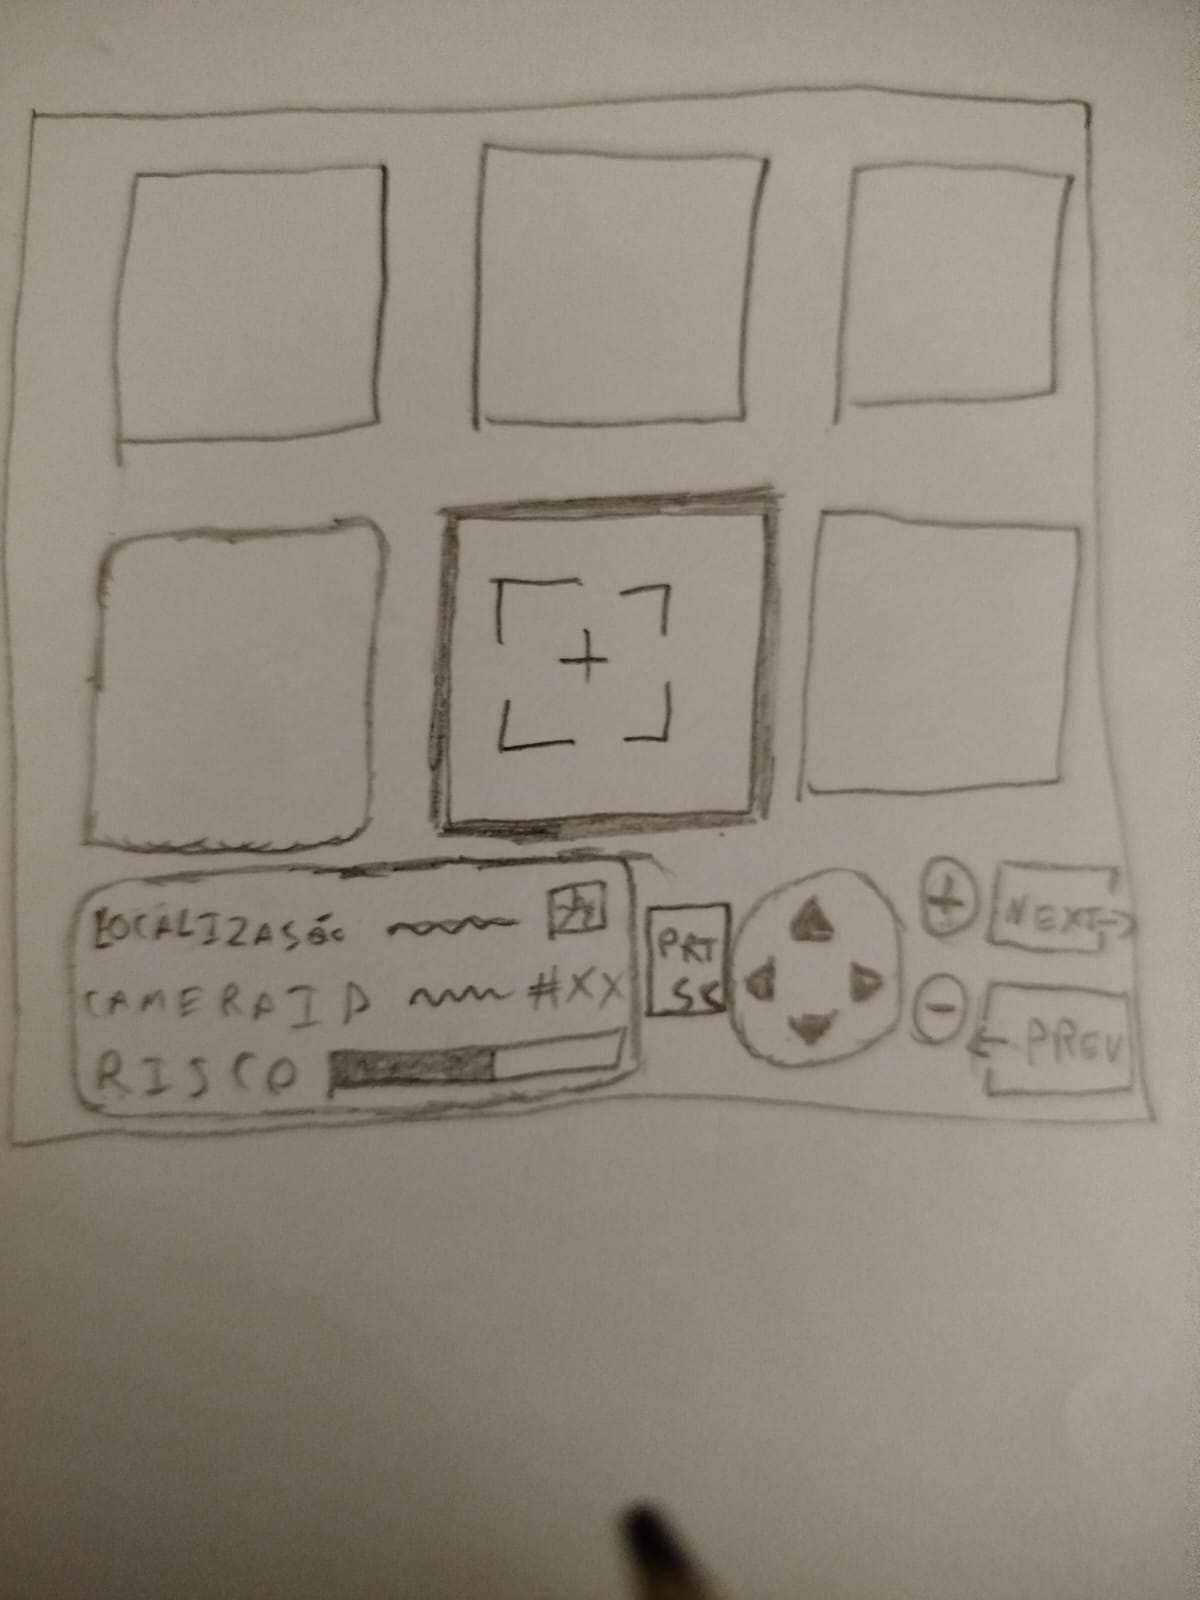
\includegraphics[width=.5\textwidth]{sketches/Resources_iter.jpg}
        \caption{Recent Camera Panel Sketch}
    \end{figure}
    \item \textbf{Resources Panel:}
\end{itemize} \par 
Upon completion of the final schematics for all the 
panels, a dashboard will be developed. The current layout 
of the dashboard is as follows:
\section{How to Interact with the Graphical Interfaces Created}
For our Situation Panel we opted for two different approaches, based on the necessity of checking areas of the map through gateways or individual sensors. \par
Both ways allow the user to check for levels of air pressure, temperature, humidity, VOCs, H2, CO and CO2 detected by the sensors. \par
It can be done either through a simplified icon display for less details, or a graphical view to check the progress of the values through a time graph. \par
In the individual Sensor portion a user would typically choose a gateway and then a specific sensor to survey their current values. \par
For the Gateway portion it was an easy choice to include a portion of the screen to display the average of the values from all of the sensors in that gateway. \par
In addition, we also thought it would be more readable to display only the selected information at a time, since all of the sensors would be displayed at the same time, therefore the user would have to choose, at the bottom of the screen, which type of levels they want to check. \par
The concept of Log Panel is to provide a comprehensive and structured repository of all information pertaining to incidents, fire states, communications, and other pertinent data that may be relevant to the civil protection operator and shared with other stakeholders. \par
In this regard, the objective is to create topics containing keywords that can be expanded upon and to ensure that all pertinent information is visible, while unnecessary details are concealed. \par
The Camera Panel enables the user to monitor six cameras simultaneously, offering a range of functions for the management and analysis of the images captured. The user may select a camera by clicking directly on its window or by utilising the Next and Prev buttons to navigate between them. The directional controls facilitate the movement of the camera and the adjustment of the zoom, according to the user's requirements. \par
The panel displays information pertaining to the location, camera ID and risk level, as determined by the sensors, represented by a progress bar. The Prt Sc button enables the capture of an image of the selected camera, which may be employed for the purposes of recording and analysis. \par
A fundamental issue for the Resources Panel is the ability to visualise the map of the area where a fire is occurring, or even multiple occurrences in a given area of the district. We also want to be able to visualise not only the outbreaks on the map, but also the resources on the ground using GPS positions. We also want to have a range of relevant information available for managing the fire, such as the number and type of air and ground resources, as well as human resources on the ground. \par
Another fundamental aspect that we tried to optimise in this iteration was to highlight the communication button, which gives access to an auxiliary screen where we can elaborate further. \par

